%% ------------------------------------------------------------------
%% AUTO-GENERATED by FlattenGlossary.py
%% Source: /Users/junga1/AaltoDictionaryofML.github.io/ADictML_Math.tex
%% Repo root: /Users/junga1/AaltoDictionaryofML.github.io
%% ------------------------------------------------------------------

\newglossaryentry{psd}
{name={positive semi-definite (psd)},
	description={A\index{positive semi-definite (psd)} (real-valued) 
		symmetric matrix $\mathbf{Q}= \mathbf{Q}\,^{T} \in \mathbb{R}^{d\times d}$ 
	 	 is referred to as psd if ${\bf x}\,^{T} \mathbf{Q}{\bf x}\geq 0$ 
		for every vector ${\bf x}\in \mathbb{R}^{d}$. 
		A psd matrix $\mathbf{Q}$ admits a spectral decomposition with nonnegative 
		eigenvalues $\lambda_{1}, \,\ldots, \,\lambda_{d} \geq 0$
		\cite{HornMatAnalysis}, \cite{Axler2025}. 
	 	The notion of being psd can be extended from matrices to (real-valued) 
	 	symmetric kernel maps $K: \mathcal{X}\times \mathcal{X}\rightarrow \mathbb{R}$ 
	 	(with $K({\bf x},{\bf x}') = K({\bf x}',{\bf x})$)
	 	as follows: For any finite set of feature vectors ${\bf x}^{(1)}, \,\ldots, \,{\bf x}^{(m)}$, 
	 	the resulting matrix $\mathbf{Q}\in \mathbb{R}^{m\times m}$ with 
		entries $Q_{r,r'} = K\big({\bf x}^{(r)},{\bf x}^{(r')}\big)$ 
		is psd \cite{LearningKernelsBook}.
			\\
		See also: symmetric matrix, kernel.},
	first={positive semi-definite (psd)},
	type=math, 
	text={psd}  
}

\newglossaryentry{normalmatrix}
{name={normal matrix},
	description={A normal matrix is a square matrix ${\bf A}\in \mathbb{C}^{d\times d}$ 
                 that commutes with its conjugate transpose, i.e., ${\bf A}{\bf A}^{H}={\bf A}^{H}{\bf A}$. 
                 Normal matrices\index{normal matrix} admit an orthonormal basis of eigenvectors and are 
                 unitarily diagonalizable.
                 \\
                 See also: matrix, diagonalizable. },
	first={normal matrix},
    	type=math, 
	plural={normal matrices},
	firstplural={normal matrices},
	text={normal matrix}
}

\newglossaryentry{spectraldecomp}
{name={spectral decomposition},
	description={Every normal matrix ${\bf A}\in \mathbb{C}^{d\times d}$ 
                 admits\index{spectral decomposition} a spectral decomposition of the form 
                 \cite{HornMatAnalysis}, \cite{Axler2025}
       		\begin{equation}
             		{\bf A}= 
              		\big( {\bf u}^{(1)}, \,\cdots, \,{\bf u}^{(d)}\big)
              		\begin{pmatrix}
              			\lambda_{1} &        &        & 0\\
                      		& \lambda_{2} &     &  \\
                      		&        & \ddots &  \\
              			0         &        &        & \lambda_{d}
		 	\end{pmatrix}
              		\begin{pmatrix}
              			\big({\bf u}^{(1)}\big)^{H}\\
             		 	\vdots\\
             			\big({\bf u}^{(d)}\big)^{H}
		 	 \end{pmatrix}
			= \sum_{j=1}^{d} \lambda_{j} {\bf u}^{(j)} \big({\bf u}^{(j)})^{H} \nonumber \\ 
       		\end{equation}
      		with an orthonormal basis ${\bf u}^{(1)},\,\ldots,\,{\bf u}^{(d)}$. 
		Each basis element ${\bf u}^{(j)}$ 
		is an eigenvector of ${\bf A}$ with a corresponding eigenvalue $\lambda_{j}$, 
		for $j=1,\,\ldots,\,d$ (see Fig. \ref{fig:eigenvectors-length_dict}).
       		\begin{figure}[H]
            		\centering
            		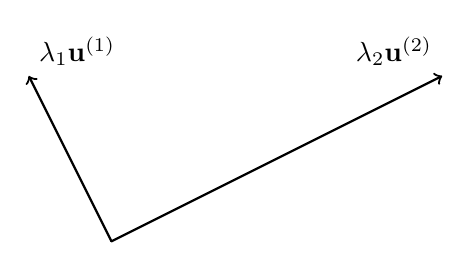
\begin{tikzpicture}[scale=2.1, line cap=round, line join=round]
            		% two eigenvectors with different lengths
            		\draw[->, thick] (0,0) -- (-0.5,1) node[above right] {$\lambda_{1} {\bf u}^{(1)}$};
           		 \draw[->, thick] (0,0) -- (2.0,1) node[above left]  {$\lambda_{2} {\bf u}^{(2)}$};
            		\end{tikzpicture}
            	\caption{The spectral decomposition of a normal matrix ${\bf A}$ provides 
			an orthonormal basis ${\bf u}^{(1)}, {\bf u}^{(2)}$. Applying ${\bf A}$ 
			amounts to a scaling of the basis vectors by the 
			eigenvalues $\lambda_{1},\lambda_{2}$.\label{fig:eigenvectors-length_dict}}
		\end{figure}
		See also: normal matrix, eigenvector, eigenvalue. },
	first={spectral decomposition},
    	type=math,
	text={spectral decomposition}
}

\newglossaryentry{symmetricmatrix}
{name={symmetric matrix},
	description={A symmetric matrix is a square\index{symmetric matrix} matrix ${\bf A}$ 
		with real-valued entries that is equal to its transpose, i.e., ${\bf A}={\bf A}^{T}$. Every 
		symmetric matrix is a normal matrix.
                 \\
                 See also: transpose, normal matrix. },
	first={symmetric matrix},
	plural={symmetric matrices},
    	type=math,
	firstplural={symmetric matrices},
	text={symmetric matrix}
}

\newglossaryentry{transpose}
{name={transpose},
	description={The transpose\index{transpose} of a real-valued matrix is obtained by exchanging 
		rows and columns. For a matrix ${\bf A}\in \mathbb{R}^{m\times d}$, 
		its transpose is denoted by ${\bf A}^{T}$ and satisfies 
		$\big({\bf A}^{T}\big)_{j,j'}=\mA_{featureidx',j}$.
		\\
		See also: matrix. },
 	first={transpose},
    	type=math, 
 	text={transpose}
 }

 \newglossaryentry{conjugatetranspose}
{name={conjugate transpose},
	description={The conjugate transpose\index{conjugate transpose} of a 
		matrix is obtained by transposing the matrix 
		and taking the complex conjugate of each entry.
		For a matrix ${\bf A}\in \mathbb{C}^{m\times d}$, its
		conjugate transpose is denoted by ${\bf A}^{H} \in 
		\mathbb{C}^{d\times m}$ and is defined entrywise by
		\[
                 ({\bf A}^{H})_{j,r}
                 = \overline{\big({\bf A}\big)_{r,j}}
		\]
		where $\overline{(\cdot)}$ denotes complex conjugation.
		\\
		See also: transpose, matrix, Hermitian. },
 	first={conjugate transpose},
    	type=math, 
 	text={conjugate transpose}
 }

\newglossaryentry{hermitian}
 {name={Hermitian},
 	description={A square\index{Hermitian} matrix ${\bf A}\in \mathbb{C}^{d\times d}$ is 
		Hermitian if it coincides with its conjugate transpose, i.e., ${\bf A}={\bf A}^{H}$. 
                 Trivially, a Hermitian matrix is also a normal matrix.
                 \\
                 See also: normal matrix. },
 	first={Hermitian},
     	type=math,
 	text={Hermitian}
}

\newglossaryentry{dimension}
{name={dimension},
	description={The\index{dimension} dimension $\dim \mathcal{A}$ of a 
		vector space $\mathcal{A}$ is the cardinality of any 
		basis of $\mathcal{A}$ \cite{StrangLinAlg2016}. 
		Strictly speaking, this definition applies only to finite-dimensional vector spaces, 
		i.e., those that possess a finite basis. 
		\begin{figure}[H]
			\begin{tikzpicture}[scale=1]
  			% Axes (optional; remove if you want it even more minimal)
  			%	\draw[->, thin, gray] (-0.2,0) -- (3.2,0) node[right] {$\vw^{(1)}$};
  			%	\draw[->, thin, gray] (0,-0.2) -- (0,3.2) node[above] {$\vw^{(1)}$};
  			\coordinate (O) at (0,0);
  			% Basis 1: standard (solid)
  			\draw[->, thick] (O) -- (1.8,0) node[below right] {${\bf e}^{(1)}$};
  			\draw[->, thick] (O) -- (0,1.6) node[above left] {${\bf e}^{(2)}$};
  			% Basis 2: rotated by ~45° (dashed)
			\draw[->, thick, dashed, shift={(3.5,0.5)}] (0,0) -- (1.2,1.2) node[above right] {${\bf u}^{(1)}$};
			\draw[->, thick, dashed, shift={(3.5,0.5)}] (0,0) -- (-1.2,1.2) node[above left] {${\bf u}^{(2)}$};
  			% Basis 3: non-orthogonal / skewed (dotted)
  			\draw[->, thick, dotted, shift={(-2.5,-2.5)}] (O) -- (2.0,0.6) node[above right] {${\bf w}^{(1)}$};
  			\draw[->, thick, dotted, shift={(-2.5,-2.5)}] (O) -- (0.4,1.8) node[left] {${\bf w}^{(2)}$};
  			% Simple legend
 			% \node[anchor=west] at (1.6,-0.6) {\footnotesize \textbf{Bases:} solid = standard,\; 
 			% dashed = rotated,\; dotted = skewed};
			\end{tikzpicture}
		\caption{Three bases, $\big\{{\bf e}^{(1)},{\bf e}^{(2)} \big\}, \big\{{\bf u}^{(1)},{\bf u}^{(2)} \big\},
			\big\{{\bf w}^{(1)},{\bf w}^{(2)} \big\}$, for the vector space $\mathbb{R}^{2}$.} 
		\end{figure}
		For such spaces, all bases have the same cardinality, which is the dimension of the space 
		\cite[Ch.~2]{Axler2025}.	
   			 \\
		See also: vector space, basis. }, 
	text={dimension}, 
	type=math,
	first={dimension}  
}

\newglossaryentry{linearlyindep}
{name={linearly independent},
	description={A subset $\{{\bf a}^{(1)}, \,\ldots, \,{\bf a}^{(d)}\} \in \mathcal{V}$ 
		of a vector space is linearly independent\index{linearly independent} 
		if there is no nontrivial linear combination of these vectors that 
		equals the zero vector \cite{StrangLinAlg2016}. 
		In other words, $$\sum_{j=1}^{d} \alpha_{j} {\bf a}^{(j)} = \mathbf{0}	
		\quad \text{ implies } \quad \alpha_{1} = \alpha_{2} = \ldots = \alpha_{k} = 0.$$ 
			\\ 
		See also: vector space, vector, dimension, basis.}, 
	text={linearly independent}, 
	type=math,
	first={linearly independent}  
}

\newglossaryentry{basis}
{name={basis},
	description={A basis\index{basis} of a finite-dimensional vector space $\mathcal{V}$ 
	             is a set of linearly independent vectors $\mathcal{B} = \{{\bf b}^{(1)}, \,\ldots, \,{\bf b}^{(d)}\} 
                 \subseteq \mathcal{V}$, such that any vector ${\bf v}\in \mathcal{V}$ 
			     can be expressed as a linear combination of the basis vectors ${\bf b}^{(1)}, \,\ldots, \,{\bf b}^{(d)}$, i.e.,	
				 $$ {\bf v}= \sum_{j=1}^{d} \alpha_{j} {\bf b}^{(j)} 
				 \quad \text{ for some } \alpha_{1}, \,\ldots, \,\alpha_{d}. $$
                 The  scalars $\alpha_{1}, \,\ldots, \,\alpha_{d} $ can be regarded 
				 as the coordinates of ${\bf v}$ with respect to the basis $\mathcal{B}$. 
				 Any basis of $\mathcal{V}$ has the same number $d$ of elements, 
				 which is the dimension of $\mathcal{V}$.
			\\
		See also: vector space, linearly independent, vector. },
	text={basis}, 
	firstplural={bases}, 
	plural={bases}, 
	type=math,
	first={basis} 
}

\newglossaryentry{widematrix}
{name={wide matrix},
	description={A\index{wide matrix} matrix 
   		${\bf X}\in \mathbb{R}^{m\times d}$ 
		is referred to as wide if it has more columns than rows, 
		i.e., when $d> m$.
		\begin{figure}[H]
			\centering
			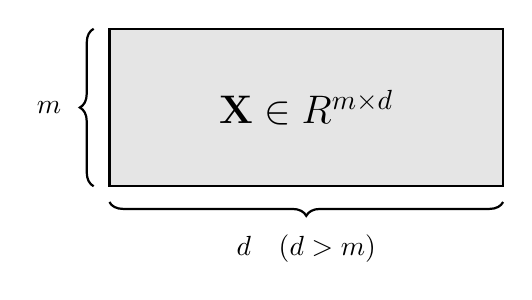
\begin{tikzpicture}
				\def\matHeight{2}
				\def\matWidth{5} 
				\draw[thick, fill=gray!20] (0,0) rectangle (\matWidth, \matHeight);
				\node at (0.5*\matWidth, 0.5*\matHeight) {\Large ${\bf X}\in \mathbb{R}^{m\times d}$};
				% vertical brace for samplesize (LEFT, correct orientation)
				\draw[decorate, decoration={brace, amplitude=5pt}, thick] 
  				(-0.2, 0) -- (-0.2, \matHeight)
  				node[midway, left=8pt] {$m$};
				\draw[decorate, decoration={brace, amplitude=5pt, mirror}, thick] 
        				(0, -0.2) -- (\matWidth, -0.2) 
        				node[midway, below=8pt] {$d\quad (d> m)$};
			\end{tikzpicture}
		\end{figure}
		See also: matrix. },
	text={wide matrix}, 
	firstplural={wide matrices}, 
	plural={wide matrices}, 
	type=math,
   	first={wide matrix} 
}

\newglossaryentry{randomexperiment}
{name={random experiment},
	description={A random experiment\index{random experiment} is a physical (or abstract) process 
    	 	that produces an outcome $\omega$ from a set $\Omega$ of possibilities. 
	 	This set of all possible outcomes is referred to as the sample space of 
	 	the experiment. The key characteristic of a random experiment is that its 
	 	outcome is unpredictable (or uncertain). Any measurement or observation 
	 	of the outcome is an random variable (RV), i.e., a function of the outcome $\omega\in \Omega$. 
	 	Probability theory uses a probability space as a mathematical structure for the study of 
	 	random experiments. A key conceptual property of a random experiment is that it can 
	 	be repeated under identical conditions. Strictly speaking, repeating a random experiment 
	 	a given number of $m$ times defines a new random experiment. The outcomes 
	 	of this new experiment are length-$m$ sequences of outcomes 
	 	from the original experiment (see Fig. \ref{fig_randomexperiment_dict}). While the outcome of a single experiment is 
	 	uncertain, the long-run behaviour of the outcomes of repeated experiments 
	 	tends to become increasingly predictable. This informal claim can be made 
	 	precise via fundamental results of probability theory, such as the law of large numbers 
	 	and the central limit theorem (CLT).
	 	\begin{figure}[H]
		\begin{center}
	 		\begin{tikzpicture}[>=Stealth, node distance=1.5cm and 2cm, every node/.style={font=\small}]
			\node (experiment) [draw, rectangle, rounded corners, minimum width=2.6cm, align=center] {random\\experiment};
			\node (omega) [right=of experiment] {$\omega\in \Omega$};
			\coordinate (rightpad) at ($(omega.east) + (0.2,0)$);
			\draw[->] (experiment) -- (omega);
			\node (sequence) [below=of experiment, yshift=-0.5cm] {$(\omega^{(1)}, \,\omega^{(2)}, \,\dots, \,\omega^{(m)})$};
			\node (sequence1) [below=of sequence, yshift=-0.5cm] {$({\bf z}^{(1)}, \,{\bf z}^{(2)}, \,\dots, \,{\bf z}^{(m)})$};
			\draw[->, thick] (experiment.south) -- node[midway, right, xshift=3pt] {repeat $m$ times} (sequence.north);
			\draw[->, thick] (sequence.south) -- node[midway, right, xshift=3pt] {random variables (RVs)} (sequence1.north);
			% Anchor node ~60% along the repeat arrow
			\path (experiment.south) -- (sequence.north) coordinate[pos=0.6] (repeatpoint);
			% Dotted rounded box enclosing experiment and part of repeat arrow
        			\node[draw=black, rounded corners, dotted, fit={(experiment) (repeatpoint) (rightpad)}, inner sep=8pt, label=above:{new random experiment with $\Omega' = \Omega\times \ldots \times \Omega$}] {};
	 		\end{tikzpicture}
	     	\end{center}
		\caption{A random experiment produces an outcome $\omega\in \Omega$ from a set 
			of possibilities (i.e., a sample space) 
			$\Omega$. Repeating the experiment $m$ times yields another random 
			experiment, whose outcomes are sequences 
			$(\omega^{(1)}, \,\omega^{(2)}, \,\dots, \,\omega^{(m)}) \in \Omega\times\ldots\times \Omega$. 
			One example of a random experiment arising in many machine learning (ML) applications is the gathering 
			of a training set ${\bf z}^{(1)},\,\ldots,\,{\bf z}^{(m)}$. \label{fig_randomexperiment_dict}}
	 	\end{figure} 
	 	Examples for random experiments arising in machine learning (ML) applications include the following: 
	 	\begin{itemize} 
			\item Data collection: The data points collected in empirical risk minimization (ERM)-based methods 
			can be interpreted as random variables (RVs), i.e., as functions of the outcome $\omega\in \Omega$ 
			of a random experiment. 
			\item Stochastic gradient descent (SGD) uses a random experiment at each iteration to select a subset of 
			the training set. 
			\item Privacy protection methods use random experiments to perturb  
			the outputs of an machine learning (ML) method to ensure DP. 
	 	\end{itemize} 
		See also: outcome, sample space, random variable (RV), probability, probability space.},
 	firstplural={random experiments},
 	plural={random experiments},
	type=math,
 	first={random experiment},
 	text={random experiment}
}

\newglossaryentry{pseudoinverse}
{name={pseudoinverse},
	description={The \index{pseudoinverse}Moore–Penrose pseudoinverse ${\bf A}^{+}$ 
 		of a matrix ${\bf X}\in \mathbb{R}^{m\times d}$ 
		generalizes the notion of an inverse matrix \cite{GolubVanLoanBook}. 
		The pseudoinverse arises naturally in ridge regression for a 
		dataset with feature matrix ${\bf X}$ and label vector 
		${\bf y}$ \cite[Ch.\ 3]{hastie01statisticallearning}. 
		The model parameters learned by ridge regression 
  		are given by
  		\[
  		\widehat{{\bf w}}^{(\alpha)}  = \big({\bf X}^{T} {\bf X}+ \alpha\mathbf{I}\big)^{-1} {\bf X}^{T} {\bf y}, \quad \alpha> 0.
  		\]
  		We can then define the pseudoinverse ${\bf X}^{+} \in \mathbb{R}^{d\times m}$ via 
  		the limit \cite[Ch. 3]{benisrael2003generalized}
  		\[
  		\lim_{\alpha\to 0^+} \widehat{{\bf w}}^{(\alpha)} = {\bf X}^+ {\bf y}.
  		\]
		\\
		See also: matrix, inverse matrix, ridge regression. },
 	first={pseudoinverse},
 	type=math, 
 	text={pseudoinverse}
} 

\newglossaryentry{tallmatrix}
{name={tall matrix},
	description={A\index{tall matrix} matrix ${\bf X}\in \mathbb{R}^{m\times d}$ 
		is referred to as tall if it has more rows than columns, i.e., 
		when $m> d$.
		\begin{figure}[H]
			\centering
			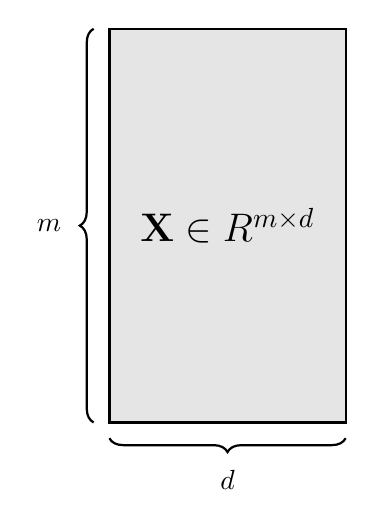
\begin{tikzpicture}
				\def\matHeight{5}
				\def\matWidth{3} 
				\draw[thick, fill=gray!20] (0,0) rectangle (\matWidth, \matHeight);
				\node at (0.5*\matWidth, 0.5*\matHeight) {\Large ${\bf X}\in \mathbb{R}^{m\times d}$};
				% vertical brace for samplesize (LEFT, correct orientation)
				\draw[decorate, decoration={brace, amplitude=5pt}, thick] 
  				(-0.2, 0) -- (-0.2, \matHeight)
  				node[midway, left=8pt] {$m$};
				\draw[decorate, decoration={brace, amplitude=5pt, mirror}, thick] 
        				(0, -0.2) -- (\matWidth, -0.2) 
        				node[midway, below=8pt] {$d$};
			\end{tikzpicture}
		\end{figure}
		See also: matrix. },
	text={tall matrix}, 
	firstplural={tall matrices}, 
	plural={tall matrices}, 
	type=math,
   	first={tall matrix} 
}

\newglossaryentry{mgf}
{name={moment generating function (MGF)}, 
	description={Consider the\index{moment generating function (MGF)} MGF $M_{x}\left(t\right)$ 
	 	of a real-valued random variable (RV) $x$, which is defined as
	 	$M_{x}\left(t\right) = \mathbb{E} \{ \exp(t \cdot x) \}$ for any $t \in \mathbb{R}$ 
	 	for which this expectation exists \cite[Sec. 21]{BillingsleyProbMeasure}. 
		As its name indicates, the MGF allows us to compute the moments 
	 	$\mathbb{E} \{ x^{k} \}$ for $k \in \mathbb{N}$. 
	 	In particular, the $k$th moment is obtained by evaluating the $k$th 
	 	derivative of $M_{x}\left(t\right)$ for $t=0$, i.e., $\mathbb{E} \{ x^{k} \} = M_{x}^{(k)}\left(0\right)$. 
	 	This fact can be verified by the following identities: 
	 	\begin{align}
			M_{x}\left(t\right) & =\mathbb{E} \{ \exp(t \cdot x)  \} \nonumber \\ 
			& \stackrel{(a)}{=} \mathbb{E} \!\bigg\{\sum_{k=0}^{\infty} \frac{t^{k}}{k!} x^{k}\bigg\}  \nonumber \\ 
			& \stackrel{(b)}{=}  \sum_{k=0}^{\infty} \frac{t^{k}}{k!}\, \mathbb{E} \!\big\{ x^{k} \big\}. \nonumber
	 	\end{align}
	 	Here, step $(a)$ is due to the Taylor series expansion of 
	 	$\exp\,(t \cdot x)$ and step $(b)$ is valid when the MGF exists 
	 	for all $t$ in some interval $(-t_{0},t_{0})$ \cite[p. 278]{BillingsleyProbMeasure}.
	 	\begin{figure}[H]
			\centering
			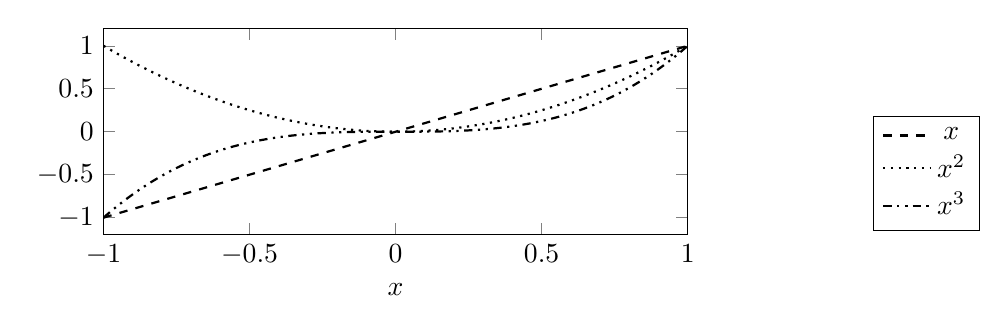
\begin{tikzpicture}
			\begin{axis}[
				width=9cm, height=4.2cm,
				domain=-1:1,
				samples=200,
				%axis lines*=left,        % removes bounding box, keeps left axis
				xlabel={$x$},
				ylabel={},
				ytick=\empty,
				ytick={-1,-0.5,0,0.5,1}, % manually set x-ticks
            			yticklabels={$-1$,$-0.5$,$0$,$0.5$,$1$},
				xtick={-1,-0.5,0,0.5,1}, % manually set x-ticks
            			xticklabels={$-1$,$-0.5$,$0$,$0.5$,$1$},
				xmin=-1, xmax=1,
				legend style={at={(1.5,0.02)},anchor=south east}
				]
				% f1 = x
				\addplot[thick, dashed] {x};
				\addlegendentry{$x$}
				% f2 = x^2
				\addplot[thick, dotted] {x^2};
				\addlegendentry{$x^{2}$}
				% f3 = x^3
				\addplot[thick, dashdotdotted] {x^3};
				\addlegendentry{$x^{3}$}
			\end{axis}
			\end{tikzpicture}
		\caption{The first few powers of an random variable (RV) $x$. The MGF 
			encodes the moments of $x$, which are the expectations 
			of the powers $x^{k}$ for $k=1,\,2,\,\ldots$.}
		\end{figure}
		The MGF is a useful tool for the study of sums of independent 
		random variables (RVs). As a case in point, if $x$ and $y$ are independent 
		random variables (RVs), then the MGF of their sum $z = x + y$ typically 
		satisfies $M_{z}\left(t\right) = M_{x}\left(t\right)\,M_{y}\left(t\right)$,
        		i.e., the MGF of the sum is typically the pointwise product of the 
		individual MGFs \cite[p.~280]{BillingsleyProbMeasure}.
		\\
 		See also: random variable (RV), expectation. }, 
 	first={moment generating function (MGF)}, 
 	firstplural={moment generating functions (MGFs)}, 
 	plural={MGFs}, 
 	type=math, 
 	text={MGF}
} 

\newglossaryentry{chernoffbound}
{name={Chernoff bound}, 
	description={The Chernoff bound\index{Chernoff bound} is a concentration inequality 
		derived as a direct application of Markov's inequality \cite[Ch.\ 2]{vershynin2018high}. 
		Let $x$ be a real-valued random variable (RV) such that its moment generating function (MGF) 
		$M_{x}\left(t\right)=\mathbb{E} \{\exp\,(t x)\}$ exists for some $t>0$. 
		Applying Markov's inequality to the nonnegative 
		random variable (RV) $\exp\,(t x)$ yields, for any $\eta\in\mathbb{R}$, 
		\begin{equation}
			\mathbb{P}\left( x\ge \eta \right)
			= \mathbb{P}\left( \exp(t x) \ge \exp(t\eta)\right)
			\le \exp(-t\eta)\, \mathbb{E} \{\exp\,(t x)\}\nonumber.
		\end{equation}
		Note that this is actually an entire family of upper bounds, parameterized 
		by all valid choices for $t>0$ (i.e., $M_{x}\left(t\right)$ must exist). 
		\\
		See also: concentration inequality, Markov's inequality, Chebyshev's inequality, 
		Hoeffding's inequality.}, 
 	first={Chernoff bound}, 
 	type=math, 
 	text={Chernoff bound}
}

\newglossaryentry{rankdeficient}
{name={rank-deficient},
	description={A matrix ${\bf A}\in \mathbb{R}^{m\times d}$ 
         	is rank-deficient\index{rank-deficient} if it is not full-rank, i.e., 
         	when $\rank{{\bf A}} < \min\{m,d\}$.
 		\begin{figure}[H]
			\begin{center}
			\begin{tikzpicture}[x=2cm]
				% LEFT: Standard basis vectors and unit square
				\begin{scope}
					\draw[->, thick] (0,0) -- (1,0) node[below] {${\bf u}^{(1)}$};
					\draw[->, thick] (0,0) -- (0,1) node[above] {${\bf u}^{(2)}$};
					%\draw[fill=gray!15] (0,0) -- (1,0) -- (1,1) -- (0,1) -- cycle;
					%\node at (0.5,0.5) {\small unit square};
					%\node at (0.5,-0.6) {standard basis};
				\end{scope}
				% RIGHT: Transformed basis vectors and parallelogram
				\begin{scope}[shift={(3.2,0)}]
				%\draw[->, thick] (0,0) -- (1,0) node[below] {$\vv^{(1)}$};
				%	\draw[->, thick] (0,0) -- (0,1) node[above] {$\vv^{(2)}$};
					\coordinate (A) at (0.2,0.0);
					\coordinate (B) at (2.0,0.0);
					\draw[->, very thick, red] (0,0) -- (A) node[below,yshift=-2pt] {${\bf A}{\bf u}^{(1)}$};
					\draw[->, very thick, red] (0,0) -- (B) node[above,yshift=2pt] {${\bf A}{\bf u}^{(2)}$};
					%	\node[blue] at (0.25,1.25) {};
					%	\node at (0.8,-0.6) {transformed basis};
				\end{scope}
				% Arrow between plots
				\draw[->, thick] (1.6,0.5) to[bend left] node[midway, above] {${\bf A}$} (2.7,0.5);
				%	\draw[->, thick] (1.3,0.5) -- (2.4,0.5) node[midway, above] {$\mA$};
			\end{tikzpicture}
			\end{center}
		\caption{Example of a rank-deficient matrix 
			${\bf A}\in \mathbb{R}^{2 \times 2}$.	\label{fig_matrix_rank_defdict}} 
		\end{figure} 
		In linear regression, the solution of the empirical risk minimization (ERM) problem is not 
		unique whenever the feature matrix ${\bf X}$ is such that 
		the matrix ${\bf X}^{\top}{\bf X}$ is rank-deficient.
		\\
   		See also: full-rank, dimension, vector space. }, 
	first={rank-deficient}, 
   	type=math,
   	text={rank-deficient}
}

\newglossaryentry{fullrank}
{name={full-rank},
 	description={A matrix ${\bf A}\in \mathbb{R}^{m\times d}$ 
  		is\index{full-rank} full-rank if it has maximum rank \cite{StrangLinAlg2016}. 
  		For a tall matrix, i.e., when $d< m$, being 
  		full-rank means that its rank is equal to $d$. 
 		\begin{figure}[H]
			\centering
			\begin{tikzpicture}[every node/.style={font=\small}]
			% --- Full-rank square ---
			\node at (0,2) {$
			{\bf A}=
			\begin{pmatrix}
			1 & 2\\
			3 & 4
			\end{pmatrix}
			$};
			\node[below=0.8cm of {$(0,2)$}] {\small full-rank square};
			% --- Rank-deficient square ---
			\node at (4.5,2) {$
			{\bf B}=
			\begin{pmatrix}
			1 & 2\\
			2 & 4
			\end{pmatrix}
			$};
			\node[below=0.8cm of {$(4.5,2)$}] {\small rank-deficient square};
			% --- Full-rank tall (3x2) ---
			\node at (0,-1.0) {$
			{\bf C}=
			\begin{pmatrix}
			1 & 0\\
			0 & 1\\
			1 & 1
			\end{pmatrix}
			$};
			\node[below=1.2cm of {$(0,-1.0)$}] {\small full-rank tall matrix};
			% --- Rank-deficient wide (2x3) ---
			\node at (4.5,-1.0) {$
			{\bf D}=
			\begin{pmatrix}
			1 & 2 & 3\\
			2 & 4 & 6
			\end{pmatrix}
			$};
			\node[below=1.2cm of {$(4.5,-1.0)$}] {\small rank-deficient wide matrix};
			\end{tikzpicture}
		\caption{Examples of full-rank and rank-deficient matrices.}
		\end{figure} 
  		A square matrix is full-rank if and only if it is invertible. 
		\\ 
  		See also: matrix, rank, dimension, linear map, column space.}, 
	text = {full-rank}, 
  	type=math,
  	first={full-rank} 
 }

\newglossaryentry{rank}
{name={rank},
	description={The rank\index{rank} of a matrix ${\bf A}\in \mathbb{R}^{m\times d}$, 
 		denoted as $\rank{{\bf A}}$, is the maximum number of linearly independent columns 
 		of ${\bf A}$ \cite{StrangLinAlg2016}. Equivalently, the rank can be defined as the 
 		dimension of the column space ${\rm span}\left({\bf A}\right) = \big\{ {\bf A}{\bf w}\mbox{ for some } 
 		{\bf w}\in \mathbb{R}^{d} \big\}$. The rank of a matrix 
 		${\bf A}\in \mathbb{R}^{m\times d}$ can neither exceed the 
 		number of rows nor the number of columns of ${\bf A}$ \cite{Horn91}, \cite{MeyerMatrixAnalysis}, 
		i.e., $\rank{{\bf A}} \leq \min \{ m, d\}$.  
		\\ 
 		See also: matrix, dimension, column space, linear map.}, 
	text={rank}, 
	type=math,
	first={rank} 
}

\newglossaryentry{inverse}
{name={inverse matrix},
	description={An inverse matrix\index{inverse matrix} ${\bf A}^{-1}$ is defined for a 
 		square matrix ${\bf A}\in \mathbb{R}^{n \times n}$ that is of full-rank, meaning its 
 		columns are linearly independent. In this case, ${\bf A}$ is said to be invertible, 
 		and its inverse satisfies 
 		\[
 		{\bf A}{\bf A}^{-1} = {\bf A}^{-1} {\bf A}= \mathbf{I}.
 		\]  	
     		A square matrix is invertible if and only if its determinant is nonzero. Inverse matrices are 
     		fundamental in solving systems of linear equations and in the closed-form solution of 
     		linear regression \cite{Strang2007}, \cite{Horn91}.  The concept of an inverse matrix can be extended 
     		to matrices that are not square or do not have full-rank. One may define a ``left inverse'' ${\bf B}$ 
     		satisfying ${\bf B}{\bf A}= \mathbf{I}$ or a ``right inverse'' ${\bf C}$ satisfying ${\bf A}{\bf C}= \mathbf{I}$. 
     		For general rectangular or singular matrices, the Moore–Penrose pseudoinverse
     		${\bf A}^{+}$ provides a unified concept of a generalized inverse matrix \cite{GolubVanLoanBook}.
 		 \begin{figure}[H]
 			\centering
 			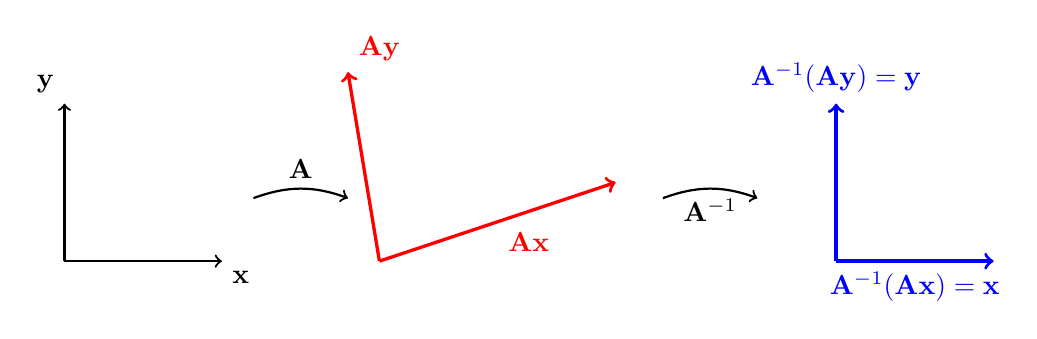
\begin{tikzpicture}[x=2cm,y=2cm]
 			% LEFT: Standard basis
 			\begin{scope}
 				\draw[->, thick] (0,0) -- (1,0) node[below right] {${\bf x}$};
 				\draw[->, thick] (0,0) -- (0,1) node[above left] {${\bf y}$};
 			\end{scope}
 			% CENTER: Transformed basis (by A)
 			\begin{scope}[shift={(2.0,0)}]
 				\coordinate (A) at (1.5,0.5);
 				\coordinate (B) at (-0.2,1.2);
				\draw[->, very thick, red] (0,0) -- (A) node[pos=0.5, below right] {${\bf A}{\bf x}$};
 				\draw[->, very thick, red] (0,0) -- (B) node[above right] {${\bf A}{\bf y}$};
 			\end{scope}
 			% RIGHT: Inverse transformation
 			\begin{scope}[shift={(4.9,0)}]
 				\draw[->, very thick, blue] (0,0) -- (1,0) node[pos=0.5, below] {${\bf A}^{-1} ({\bf A}{\bf x}) = {\bf x}$};
 				\draw[->, very thick, blue] (0,0) -- (0,1) node[above] {${\bf A}^{-1} ({\bf A}{\bf y}) = {\bf y}$};
 			\end{scope}
 			% Curved arrows between stages
 			\draw[->, thick, bend left=20] (1.2,0.4) to node[above] {${\bf A}$} (1.8,0.4);
 			\draw[->, thick, bend left=20] (3.8,0.4) to node[below] {${\bf A}^{-1}$} (4.4,0.4);
 			\end{tikzpicture}
 		\caption{A matrix $\mathbf{A}$ represents a linear transformation of $\mathbb{R}^{2}$. The inverse matrix $\mathbf{A}^{-1}$ 
 			represents the inverse transformation. \label{fig_matrix_inverse_dict}} 
 		\end{figure}
		See also: matrix, determinant, linear regression, pseudoinverse.},
	first={inverse matrix},
	type=math,
	text={inverse matrix}
}

\newglossaryentry{matrix}
{name={matrix},
	description={A matrix\index{matrix} of size $m\times d$ is a 2-D array of numbers, 
 		which is denoted by 
		$$
  		{\bf A}= \begin{pmatrix}
   		A_{1,1} & A_{1,2} & \dots  & A_{1,d} \\
		A_{2,1} & A_{2,2} & \dots  & A_{2,d} \\
		\vdots  & \vdots  & \ddots & \vdots \\
		A_{m,1} & A_{m,2} & \dots  & A_{m,d}
		\end{pmatrix} \in \mathbb{R}^{m\times d}.
		$$
		Here, $A_{r,j}$ denotes the matrix entry in the $r$th row and the 
		$j$th column. Matrices are useful representations of various mathematical objects \cite{StrangLinAlg2016},
		including the following:
		\begin{itemize}
			\item Systems of linear equations: We can use a matrix to represent a system of linear equations 
			$$ \begin{pmatrix}
			A_{1,1} & A_{1,2} \\
			A_{2,1} & A_{2,2}
			\end{pmatrix}
			\begin{pmatrix}
				w_1 \\
				w_2
			\end{pmatrix}
			=\begin{pmatrix}
				y_1 \\
				y_2
			\end{pmatrix}
			\quad \text{ compactly as } \quad {\bf A}{\bf w}= {\bf y}.
			$$
    			One important example of systems of linear equations is the optimality condition for the 
    			model parameters within linear regression. 
			\item Linear maps:
			Consider a $d$-dimensional vector space $\mathcal{U}$ and a $m$-dimensional vector space $\mathcal{V}$. 
			If we fix a basis $\mathbf{u}^{(1)},\,\ldots,\,\mathbf{u}^{(d)}$ for $\mathcal{U}$ and a basis $\mathbf{v}^{(1)},\,\ldots,\,\mathbf{v}^{(m)}$ 
			for $\mathcal{V}$, each matrix ${\bf A}\in \mathbb{R}^{m\times d}$ naturally defines a 
			linear map $\alpha: \mathcal{U} \rightarrow \mathcal{V}$ (see Fig. \ref{fig_matrix_dict}) such that
   			$${\bf u}^{(j)} \mapsto \sum_{r=1}^{m} A_{r,j} {\bf v}^{(r)}.$$
			\item Datasets: We can use a matrix to represent a dataset. Each row 
			corresponds to a single data point, and each column corresponds to a specific 
			feature or label of a data point. 
		\end{itemize}
		\begin{figure}[H]
		\begin{center}
		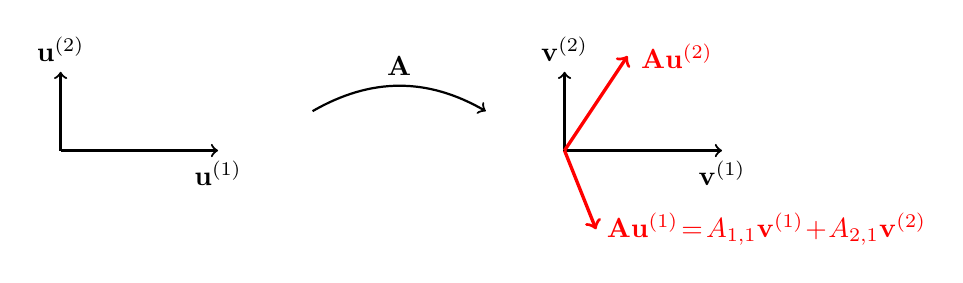
\begin{tikzpicture}[x=2cm]
			% LEFT: Standard basis vectors and unit square
			\begin{scope}
				\draw[->, thick] (0,0) -- (1,0) node[below] {${\bf u}^{(1)}$};
				\draw[->, thick] (0,0) -- (0,1) node[above] {${\bf u}^{(2)}$};
				%\draw[fill=gray!15] (0,0) -- (1,0) -- (1,1) -- (0,1) -- cycle;
				%\node at (0.5,0.5) {\small unit square};
				%\node at (0.5,-0.6) {standard basis};
			\end{scope}
			% RIGHT: Transformed basis vectors and parallelogram
			\begin{scope}[shift={(3.2,0)}]
				\draw[->, thick] (0,0) -- (1,0) node[below] {${\bf v}^{(1)}$};
				\draw[->, thick] (0,0) -- (0,1) node[above] {${\bf v}^{(2)}$};
				\coordinate (A) at (0.2,-1.0);
				\coordinate (B) at (0.4,1.2);
				\draw[->, very thick, red] (0,0) -- (A) node[below,right] {${\bf A}{\bf u}^{(1)}\!=\!A_{1,1}{\bf v}^{(1)}\!+\!A_{2,1}{\bf v}^{(2)}$};
				\draw[->, very thick, red] (0,0) -- (B) node[right,xshift=1pt] {${\bf A}{\bf u}^{(2)}$};
				%	\node[blue] at (0.25,1.25) {};
				%	\node at (0.8,-0.6) {transformed basis};
			\end{scope}
			% Arrow between plots
			\draw[->, thick] (1.6,0.5) to[bend left] node[midway, above] {${\bf A}$} (2.7,0.5);
		%	\draw[->, thick] (1.3,0.5) -- (2.4,0.5) node[midway, above] {$\mA$};
		\end{tikzpicture}
		\end{center}
		\caption{A matrix ${\bf A}$ defines a linear map between two vector spaces. \label{fig_matrix_dict}} 
		\end{figure}
		See also: linear map, dataset, linear model. },
	first={matrix},
	firstplural={matrices},
	type=math,
	plural={matrices},
	text={matrix}
}

\newglossaryentry{hyperplane}
{name={hyperplane},
	description={A hyperplane\index{hyperplane} is an $(d-1)$-dimensional affine 
		subspace of a $d$-dimensional vector space. In the 
		context of a Euclidean space $\mathbb{R}^{d}$, a 
		hyperplane is a set of the form
 		\[ 
		\{ {\bf x}\in \mathbb{R}^d: {\bf w}^\top {\bf x}= b \}
  		\]
                 where ${\bf w}\in \mathbb{R}^d \setminus \{0\}$ is a normal vector 
                 and $b \in \mathbb{R}$ is an offset. Such a hyperplane partitions 
		$\mathbb{R}^d$ into two halfspaces
		\[\{ {\bf x}\in \mathbb{R}^d: {\bf w}^\top {\bf x}\leq b \} \quad 
		\text{and} \quad \{ {\bf x}\in \mathbb{R}^d: {\bf w}^\top {\bf x}\geq b \}.\]
 		Hyperplanes arise as the decision boundaries of linear classifiers.
		\\
		See also: subspace, vector space, Euclidean space, decision boundary. },
	first={hyperplane},
	type=math,
	plural={hyperplanes}, 
	firstplural={hyperplanes},
	text={hyperplane}
}

\newglossaryentry{normalvector}
{name={normal vector},
	description={See\index{normal vector} hyperplane.},
	first={normal vector},
	type=math,
	plural={normal vectors}, 
	firstplural={normal vectors},
	text={normal vector}
}

\newglossaryentry{halfspace}
{name={halfspace},
	description={See\index{halfspace} hyperplane.},
	first={halfspace},
	type=math,
	plural={halfspaces}, 
	firstplural={halfspaces},
	text={halfspace}
}

\newglossaryentry{subspace}
{name={subspace},
	description={A subset of a vector space $\mathcal{V}$ is a subspace\index{subspace} of $\mathcal{V}$ if it is also a 
		vector space with respect to the same operations as $\mathcal{V}$.
			   \\
		See also: vector space.},
	type=math, 
	first={subspace},
	text={subspace}
}

\newglossaryentry{columnspace}
{name={column space},
	description={The column space\index{column space} of a matrix 
		${\bf A}\in \mathbb{R}^{m\times d}$,
		denoted by ${\rm span}\left({\bf A}\right)$, is the set of all linear combinations of the 
		columns of ${\bf A}$. In other words, 
		$$ {\rm span}\left({\bf A}\right) = \{ {\bf A}{\bf w}: {\bf w}\in \mathbb{R}^{d} \}. $$
		The column space ${\rm span}\left({\bf A}\right)$ of the matrix ${\bf A}$ 
		is a subspace of the Euclidean space $\mathbb{R}^{m}$.
			   \\
		See also: matrix, vector space.},
	type=math,
	first={column space},
	text={column space}
}

\newglossaryentry{mvndist}
{name={multivariate normal distribution}, 
	description={The\index{multivariate normal distribution} multivariate normal distribution, 
		which is denoted by $\mathcal{N}\left({\bm \mu},{\bf C}\right)$, is a fundamental 
		probabilistic model for numerical feature vectors of fixed dimension $d$. 
		It defines a family of probability distributions over vector-valued random variables (RVs) 
		${\bf x}\in \mathbb{R}^{d}$~\cite{BertsekasProb}, \cite{GrayProbBook}, \cite{Lapidoth09}. 
		Each distribution in this family is fully specified by its mean vector 
		${\bm \mu}\in \mathbb{R}^{d}$ and covariance matrix 
		${\bf C}\in \mathbb{R}^{d\times d}$. When the 
		covariance matrix ${\bf C}$ is invertible, the corresponding probability distribution is 
		characterized by the following probability density function (pdf):
		\[p({\bf x}) = 
 		\frac{1}{\sqrt{(2\pi)^{d} \det\,({\bf C})}} 
 		\exp\left[ -\frac{1}{2} 
 		({\bf x}- {\bm \mu})\,^{T}\, {\bf C}^{-1} 
 		({\bf x}- {\bm \mu}) \right].
 		\]
		Note that this probability density function (pdf) is only defined when ${\bf C}$ is invertible.
   		More generally, any random variable (RV) ${\bf x}\sim \mathcal{N}\left({\bm \mu},{\bf C}\right)$ 
   		admits the following representation:
  		\[
    		{\bf x}= {\bf A}{\bf z}+ {\bm \mu}\]
   		where ${\bf z}\sim \mathcal{N}\left(\mathbf{0},\mathbf{I}\right)$ is a standard normal random vector 
   		and ${\bf A}\in \mathbb{R}^{d\times d}$ satisfies ${\bf A}{\bf A}^\top = {\bf C}$. 
   		This representation remains valid even when ${\bf C}$ is singular, in which case ${\bf A}$ 
   		is not full-rank~\cite[Ch. 23]{Lapidoth2017}.
   		The family of multivariate normal distributions is exceptional among probabilistic models for numerical 
   		quantities, at least for the following reasons. First, the family is closed under affine 
   		transformations, i.e.,
		\[ 
		{\bf x}\sim \mathcal{N}({\bm \mu},{\bf C}) \mbox{ implies } 
		{\bf B}{\bf x}\!+\!{\bf c}\sim \mathcal{N}\big( {\bf B}{\bm \mu}+{\bf c},{\bf B}{\bf C}{\bf B}\,^{T} \big). 
		\]
		Second, the probability distribution $\mathcal{N}(\mathbf{0},{\bf C})$ maximizes the 
		differential entropy among all distributions with the same covariance matrix ${\bf C}$~\cite{coverthomas}. 
		\\ 
		See also: probabilistic model, probability distribution, standard normal random vector, differential entropy, Gaussian random variable (Gaussian RV).}, 
	first={multivariate normal distribution},
	type=math, 
	text={multivariate normal distribution}
}

\newglossaryentry{stdnormvec}
{name={standard normal random vector}, 
	description={A\index{standard normal random vector} standard normal random vector 
		is an random variable (RV) ${\bf x}=\big(\feature_{1}, \,\ldots, \,\feature_{d}\big)\,^{T}$ 
		whose entries are independent and identically distributed (i.i.d.) Gaussian random variables (Gaussian RVs) $x_{j} \sim \mathcal{N}(0,1)$. 
		The probability distribution of a standard normal random vector is a special case 
		of a multivariate normal distribution ${\bf x}\sim \mathcal{N}(\mathbf{0},\mathbf{I})$.
		\\ 
		See also: vector, independent and identically distributed (i.i.d.), Gaussian random variable (Gaussian RV), multivariate normal distribution, random variable (RV).}, 
	first={standard normal random vector},
	type=math, 
	text={standard normal random vector}
}

\newglossaryentry{continuous}
% This is perfectly fine, of course, to give the epsilon-delta-definition of continuity. The (equivalent) definition using  
% limits is perhaps though easier to understand, so it could be an alternative and could at least be briefly mentioned - 
% but  of course, just a remark, perfectly fine as it is.
{name={continuous}, 
	description={A function\index{continuous} $f: \mathbb{R}^{d} \to \mathbb{R}$ is 
		continuous at a point ${\bf x}' \in \mathbb{R}^{d}$ if, for 
	 	every $\epsilon > 0$, there is a $\delta > 0$ such that, for all 
	 	${\bf x}\in \mathbb{R}^{d}$ with $\mleft\lVert {\bf x}- {\bf x}' \mright\rVert_{2} < \delta$, 
	 	it holds that $|f({\bf x}) - f({\bf x}')| < \epsilon$ \cite{RudinBookPrinciplesMatheAnalysis}. 
	 	In other words, we can make $f({\bf x})$ arbitrarily close to $f({\bf x}')$ 
	 	by choosing ${\bf x}$ sufficiently close to ${\bf x}'$. 
		\begin{figure}[H]
			\centering
	 		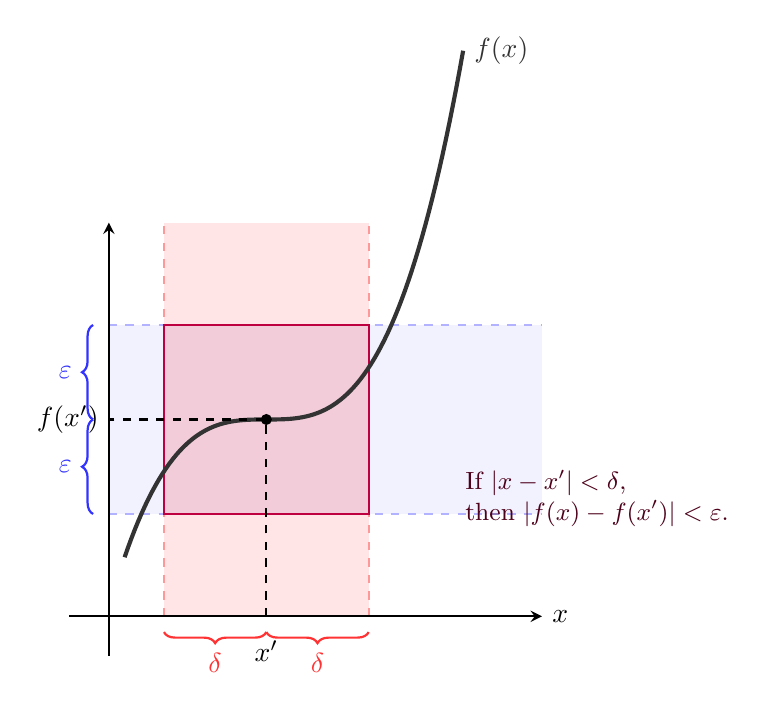
\begin{tikzpicture}[
				>=stealth, 
    				thick,
				%f(x) = 0.5(x-2)^3 + 2
    				declare function={f(\x) = 0.3*(\x-2)^3 + 2.5;}
				]
				\def\xprime{2}      % x'
    				\def\epsilonval{1.2}   % epsilon
				\def\deltaval{1.3}     % delta
				\def\xmax{5.5}
				\def\ymax{5}
				\fill[blue!5] (0, {f(\xprime)-\epsilonval}) rectangle (\xmax, {f(\xprime)+\epsilonval});
				\draw[blue!30, dashed] (0, {f(\xprime)-\epsilonval}) -- (\xmax, {f(\xprime)-\epsilonval});
				\draw[blue!30, dashed] (0, {f(\xprime)+\epsilonval}) -- (\xmax, {f(\xprime)+\epsilonval});
				\fill[red!10] ({\xprime-\deltaval}, 0) rectangle ({\xprime+\deltaval}, \ymax);
				\draw[red!40, dashed] ({\xprime-\deltaval}, 0) -- ({\xprime-\deltaval}, \ymax);
				\draw[red!40, dashed] ({\xprime+\deltaval}, 0) -- ({\xprime+\deltaval}, \ymax);
				\fill[purple!20] ({\xprime-\deltaval}, {f(\xprime)-\epsilonval}) rectangle ({\xprime+\deltaval}, {f(\xprime)+\epsilonval});
				\draw[purple, thick] ({\xprime-\deltaval}, {f(\xprime)-\epsilonval}) rectangle ({\xprime+\deltaval}, {f(\xprime)+\epsilonval});
				\draw[->] (-0.5,0) -- (\xmax,0) node[right] {$x$};
				\draw[->] (0,-0.5) -- (0,\ymax) node[above] {};
				% The Function 
				\draw[line width=1.5pt, black!80] plot[domain=0.2:4.5, samples=100] (\x, {f(\x)}) 
				node[right] {$f(x)$};
				\draw[dashed] (\xprime, 0) -- (\xprime, {f(\xprime)}) -- (0, {f(\xprime)});
				\fill[black] (\xprime, {f(\xprime)}) circle (2pt);
				\node[below,yshift=-5pt] at (\xprime, 0) {$x'$};
				\node[left] at (0, {f(\xprime)}) {$f(x')$};
				\draw[decorate, decoration={brace, amplitude=4pt}, blue!80] 
				(-0.2, {f(\xprime)}) -- (-0.2, {f(\xprime)+\epsilonval}) 
				node[midway, left=4pt] {$\varepsilon$};
				\draw[decorate, decoration={brace, amplitude=4pt}, blue!80] 
				(-0.2, {f(\xprime)-\epsilonval}) -- (-0.2, {f(\xprime)}) 
				node[midway, left=4pt] {$\varepsilon$};
				\draw[decorate, decoration={brace, amplitude=4pt, mirror}, red!80] 
				(\xprime, -0.2) -- ({\xprime+\deltaval}, -0.2) 
				node[midway, below=4pt] {$\delta$};
				\draw[decorate, decoration={brace, amplitude=4pt, mirror}, red!80] 
				({\xprime-\deltaval}, -0.2) -- (\xprime, -0.2) 
				node[midway, below=4pt] {$\delta$};
				\node[align=left, purple!40!black, font=\small] at (6.2, 1.5) 
				{If $| x- x' | < \delta$,\\
				then $| f(x) - f(x') | < \varepsilon$.};
			\end{tikzpicture}
		\caption{The function $f(x) = 0.3(x-2)^3 + 2.5$ is continuous 
		         at every $x'$.}
		\end{figure}
		If $f$ is continuous at every point ${\bf x}' \in \mathbb{R}^{d}$, then $f$ is said to be 
	 	continuous on $\mathbb{R}^{d}$. The notion of a continuous 
	 	function can be naturally extended to functions between general metric spaces 
		\cite{RudinBookPrinciplesMatheAnalysis}.
		\\
		See also: Euclidean space, metric.},
	first={continuous},
	type=math,
	text={continuous}
}

\newglossaryentry{minimum}
{name={minimum},
	description={Given a set of real numbers, the minimum\index{minimum} is the smallest of those numbers.
		Note that for some sets, such as the set of negative real numbers, the minimum does not exist.},
	firstplural={minima}, 
 	plural={minima},
	type=math, 
	first={minimum},
	text={minimum}
}

\newglossaryentry{co-domain}
{name={co-domain}, 
	description={The co-domain\index{co-domain} of a function 
		$f: \mathcal{U} \rightarrow \mathcal{V}$ is the set $\mathcal{V}$ 
		into which $f$ maps elements of its domain $\mathcal{U}$.  
		\begin{figure}[H]
			\centering
			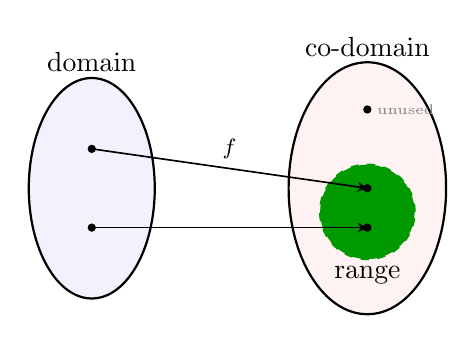
\begin{tikzpicture}[
			>=stealth, 
			node distance=2cm,
			scale=1.0, every node/.style={transform shape} % Scales the whole diagram down slightly
			]
			% Domain A
			\draw[thick, fill=blue!5] (0,0) ellipse (0.8cm and 1.4cm);
			\node[] at (0, 1.6) {domain};
			% Codomain B
			\draw[thick, fill=red!5] (3.5,0) ellipse (1cm and 1.6cm);
			\node[] at (3.5, 1.8) {co-domain};
			\draw[dashed, fill=green!10, thick, green!60!black] (3.5, -0.3) circle (0.6cm);
			\node[] at (3.5, -1.1) {range};
			\fill (0, 0.5) circle (1.5pt) coordinate (a1);
			\fill (0, -0.5) circle (1.5pt) coordinate (a2);
			% Output points
			\fill (3.5, 0) circle (1.5pt) coordinate (b1);
			\fill (3.5, -0.5) circle (1.5pt) coordinate (b2);
			% Unreached point
			\fill (3.5, 1.0) circle (1.5pt) coordinate (b_miss) node[right, font=\tiny, gray] {unused};
			\draw[->, semithick] (a1) -- (b1);
			\draw[->, semithick] (a2) -- (b2);
			% Function Label
			\node[font=\footnotesize] at (1.75, 0.5) {$f$};
			\end{tikzpicture}
		\end{figure}
		See also: domain, function, map.},
	first={co-domain},
	firstplural={co-domains}, 
	type=math, 
	plural={co-domains},
	text={co-domain}
}

\newglossaryentry{cdf}
{name={cumulative distribution function (cdf)},
	description={The \index{cumulative distribution function (cdf)} cdf 
		$F^{(x)}\left(\eta\right)$ of a real-valued random variable (RV) $x$ is \cite{AshProbMeasure}, \cite{papoulis}
		$$F^{(x)}\left(\eta\right) :=\mathbb{P}\left(x\leq \eta\right).$$
					\\ 
		See also: random variable (RV), probability density function (pdf), probability distribution.},
	first={cumulative distribution function (cdf)},
	firstplural={cumulative distribution functions (cdfs)}, 
	plural={cdfs}, 
	type=math,
	text={cdf} 
}

\newglossaryentry{weightedgraph}
{name={weighted graph},
	description={A weighted graph is a graph\index{weighted graph} whose edges 
		are assigned numeric weights. Typically, these edge weights 
		are nonnegative real numbers. For example, if a graph represents 
		a road network with nodes corresponding to intersections and edges representing 
		road segments, the edge weight could represent the capacity (measured 
		in maximum vehicles per hour) of the road segment \cite{NewmannBook}.  
		\begin{figure}[H] 
			\centering
			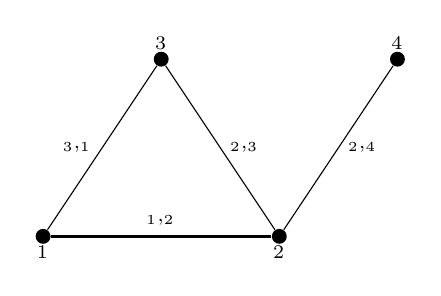
\begin{tikzpicture}[scale=1.5,
				node/.style={circle, fill=black, inner sep=1.9pt},
				lab/.style={anchor=west, xshift=3pt}
				]
				% Nodes (points)
				\node[node] (v1) at (0,0) {};
				\node[node] (v2) at (2,0) {};
				\node[node] (v3) at (1,1.5) {};
				\node[node] (v4) at (3,1.5) {};
				% Labels
				\node[anchor=north] at (v1) {$\nodeidx_1$};
				\node[anchor=north] at (v2) {$\nodeidx_2$};
				\node[anchor=south] at (v3) {$\nodeidx_3$};
				\node[anchor=south] at (v4) {$\nodeidx_4$};
				% Undirected edges
				\draw [line width=1pt] (v1) -- node[midway, above] {$\edgeweight_{\nodeidx_1,\nodeidx_2}$} (v2);
				\draw (v2) -- node[midway, right] {$\edgeweight_{\nodeidx_2,\nodeidx_3}$} (v3);
				\draw (v3) -- node[midway, left] {$\edgeweight_{\nodeidx_3,\nodeidx_1}$} (v1);
				\draw (v2) -- node[midway, right] {$\edgeweight_{\nodeidx_2,\nodeidx_4}$} (v4);
			\end{tikzpicture}
		\caption{A weighted graph with four nodes 
			$\mathcal{V}= \{\nodeidx_1, \nodeidx_2, \nodeidx_3, \nodeidx_4\}$ 
			and four edges $\mathcal{E}= \{\{\nodeidx_1,\nodeidx_2\},
			\{\nodeidx_2,\nodeidx_3\}, \{\nodeidx_3,\nodeidx_1\}, 
			\{\nodeidx_2,\nodeidx_4\}\}$. Each edge is assigned a weight.}
		\end{figure}		
		See also: graph.},
	first={weighted graph},
	type=math,
	firstplural={weighted graphs}, 
	plural={weighted graphs}, 
	text={weighted graph} 
}

\newglossaryentry{graph}
{name={graph},
	description={A graph\index{graph} $\mathcal{G}= \left( \mathcal{V},\mathcal{E}\right)$ 
		consists of a node set $\mathcal{V}$ and an edge set $\mathcal{E}$.
		Each edge $e\in \mathcal{E}$ is characterized by the nodes to which 
		it is connected and in what precise sense. For example, 
		an edge of a directed graph is leaving one node 
		and pointing to another node. An edge of an undirected graph 
		connects two nodes without any sense of 
		direction \cite{NewmannBook}, \cite{RockNetworks}. 
		In principle, there can also be several (parallel) edges that are 
		connected to the same nodes in the same way \cite{RockNetworks}. 
		Moreover, edges may connect a node to itself, resulting in 
		so-called self-loops \cite{NewmannBook}. 
		A simple undirected graph contains no 
		parallel edges and no self-loops \cite{WilsonGraph2010}. 
		Each edge $e\in \mathcal{E}$ of a simple undirected graph
		can be identified with a set of two nodes ${i,i'}$. 
		\begin{figure}[H] 
			\centering
			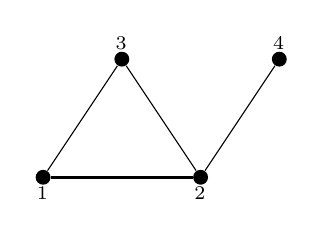
\begin{tikzpicture}[scale=1,
				node/.style={circle, fill=black, inner sep=1.9pt},
				lab/.style={anchor=west, xshift=3pt}
				]
				% Nodes (points)
				\node[node] (v1) at (0,0) {};
				\node[node] (v2) at (2,0) {};
				\node[node] (v3) at (1,1.5) {};
				\node[node] (v4) at (3,1.5) {};
				% Labels
				\node[anchor=north] at (v1) {$\nodeidx_1$};
				\node[anchor=north] at (v2) {$\nodeidx_2$};
				\node[anchor=south] at (v3) {$\nodeidx_3$};
				\node[anchor=south] at (v4) {$\nodeidx_4$};
				% Undirected edges
				\draw [line width=1pt] (v1) -- (v2);
				\draw (v2) -- (v3);
				\draw (v3) -- (v1);
				\draw (v2) -- (v4);
			\end{tikzpicture}
		\caption{A simple undirected graph with four nodes 
			$\mathcal{V}= \{\nodeidx_1, \nodeidx_2, \nodeidx_3, \nodeidx_4\}$ 
			and four edges $\mathcal{E}= \{\{\nodeidx_1,\nodeidx_2\},
			\{\nodeidx_2,\nodeidx_3\}, \{\nodeidx_3,\nodeidx_1\}, 
			\{\nodeidx_2,\nodeidx_4\}\}$.}
		\end{figure}
		Weighted graphs assign a numerical value $\edgeweight_{e}$, 
		referred to as edge weight, to each edge $e\in \mathcal{E}$.
					\\ 
		See also: map, edge weight.},
 	first={graph},
 	text={graph}, 
 	firstplural={graphs}, 
	plural={graphs}, 
 	type=math
}

\newglossaryentry{markovchain}
{name={Markov chain},
	description={A Markov chain\index{Markov chain} is a stochastic process $\{X_t\}_{t\in \mathbb{N}}$ 
		defined on a common probability space and using the index set $\mathbb{N}$. The 
		random variable (RV) $X_t$ might represent (the generation of) a state of a physical system 
		at the time instant $t$. The defining property of a Markov chain 
		is the Markov property \cite{durrett2010probability}, \cite{papoulis}, \cite{NorrisMarkovChains1997}.
		For all $t\in \mathbb{N}$,
 		\begin{equation}
 			\nonumber \mathbb{P}^{(X_{t+1} \mid X_t,\ldots,X_1)} = \mathbb{P}^{(X_{t+1} \mid X_t)}. 
 		\end{equation}
 		In other words, the conditional probability distribution of the next state $X_{t+1}$ 
		depends on the past $X_{t},X_{t-1},\,\dots,\,X_{1}$ 
		only through the current state $X_{t}$. The concept of a 
		Markov chain can be generalized from discrete time (with index set $\mathbb{N}$) 
		to continuous time (with index set $\mathbb{R}$) \cite{NorrisMarkovChains1997}. 
		\\ 
		See also: stochastic process, conditional probability distribution.},
	first={Markov chain},
	type=math,
    	text={Markov chain}, 
	plural={Markov chains}, 
	firstplural={Markov chains}
}

\newglossaryentry{markovprop}
{name={Markov property},
	description={See Markov chain\index{Markov property}.},
	first={Markov property},
	type=math,
	text={Markov property}
}

\newglossaryentry{em}
{name={expectation–maximization (EM)}, 
	description={\index{expectation–maximization (EM)}
	    	The EM algorithm \cite{dempster1977maximum} is an iterative optimization method for 
		approximately solving certain maximum likelihood optimization problems 
		that are difficult to solve directly \cite[Sec. 9.4]{BishopBook}, \cite[Sec. 11.4.7]{Murphy2012}.
	    	To motivate the EM algorithm and explain its construction, 
		consider an machine learning (ML) application involving a single observed data point 
		with feature $x\in \mathcal{X}$, where $\mathcal{X}$ 
		is a finite feature space. The data generation 
		is modeled via a probabilistic model that consists of an random variable (RV) $x'$ 
		with probability mass function (pmf) $p^{(x')}\left(\cdot;{\bf w}\right)$. Here, 
		the actual model parameters ${\bf w}\in \mathcal{W}$—used for the data 
		generation via sampling from $p^{(x')}\left(\cdot;{\bf w}\right)$—are unknown. A widely 
		used approach for estimating these model parameters is via the solutions of the maximum likelihood 
		problem
		\begin{equation}
			\label{equ_def_ML_EM_dict}
			\min_{{\bf w}\in \mathcal{W}} - \log p^{(x')}\left(x;{\bf w}\right).
		\end{equation}
		For some probabilistic models, such as a Gaussian mixture model (GMM), this optimization problem can be 
		difficult to solve directly. As a work-around, one can often introduce an auxiliary 
		attribute $y\in \mathcal{Y}$, generated via some random variable (RV) $y'$, 
		such that the corresponding probabilistic model $p^{(x',y')}\left(\cdot,\cdot;{\bf w}\right)$ 
		yields a much easier maximum likelihood problem 
		\begin{equation}
			\label{equ_def_complete_EM_dict}
			\min_{{\bf w}\in \mathcal{W}} 
			- \log p^{(x',y')}\left(x,y;{\bf w}\right).
		\end{equation}
		The attribute $y$ is introduced solely to simplify 
		\eqref{equ_def_complete_EM_dict}, but it is not observed in practice—only the 
		feature $x$ is available. Thus, we cannot solve \eqref{equ_def_complete_EM_dict} 
		directly as we do not know which value $y$ to plug into the probability mass function (pmf) 
		$ p^{(x',y')}\left(x,y;{\bf w}\right)$. 
		The EM method resolves this dilemma by alternating between the following two steps:
		1) an E-step, in which a “soft’’ estimate of the auxiliary attribute $y$ is computed 
		in the form of the posterior $p^{(y'|x')}\left(\cdot;\widehat{{\bf w}}\right)$
		using the current choice $\widehat{{\bf w}}$ for the model parameters; and 
		2) an M-step, in which a surrogate objective function derived from this posterior is minimized.
		The completion of these two steps constitutes one full iteration of 
		the EM method. 
		In more detail, the E-step produces the function
		\[
		Q({\bf w}\mid \widehat{{\bf w}})
		:=- \sum_{y\in \mathcal{Y}} 
		p^{(y'|x')}\left(y;\widehat{{\bf w}}\right)
		\log\!\Big(
		p^{(x',y')}\left(x,y;{\bf w}\right)
		/p^{(y'|x')}\left(y;\widehat{{\bf w}}\right)
		\Big)
		\]
		and the M-step minimizes $Q({\bf w}\mid \widehat{{\bf w}})$ over 
		${\bf w}\in \mathcal{W}$.
		This function satisfies the following two key properties 
		\cite[Sec. 9.4]{BishopBook},\cite[Sec. 11.4.7]{Murphy2012}:
		1) upper bound
		$Q({\bf w}\mid \widehat{{\bf w}})
		\geq
		- \log p^{(x')}\left(x;{\bf w}\right)$,
		for all ${\bf w}\in \mathcal{W}$;
		and 2) tightness
		$Q(\widehat{{\bf w}}\mid \widehat{{\bf w}})
		=- \log p^{(x')}\left(x;\widehat{{\bf w}}\right).$
		To summarize, during each iteration, EM minimizes an upper-bounding 
		surrogate objective function that is tight at the current iterate $\widehat{{\bf w}}$. 
		Thus, EM is a majorize–minimize (MM) method for approximately solving \eqref{equ_def_ML_EM_dict}. 
		The above construction and analysis of EM can be extended to more 
		general settings involving multiple data points 
		and infinite feature spaces such as $\mathbb{R}^{d}$ 
		(see \cite[Sec. 11.4.7]{Murphy2012} for further details). 
			\\
		See also: maximum likelihood, optimization problem, probabilistic model. },
	first={expectation–maximization (EM)},
	type=math, 
	text={EM}
}

\newglossaryentry{ppca}
{name={probabilistic principal component analysis (PPCA)}, 
	description={PPCA\index{probabilistic principal component analysis (PPCA)} 
		extends basic principal component analysis (PCA) by using a probabilistic model for data points. 
		Using a probabilistic model allows to cast dimensionality reduction as an estimation problem 
		that can be solved using expectation–maximization (EM) \cite{TippingProbPCA}.
				\\
		See also: principal component analysis (PCA), probabilistic model, dimensionality reduction, expectation–maximization (EM).},
	first={probabilistic principal component analysis (PPCA)},
	type=math, 
	text={PPCA}
}

\newglossaryentry{contractop}
{name={contractive operator},
	description={An\index{contractive operator} operator 
		$\mathcal{F}: \mathbb{R}^{d} \rightarrow \mathbb{R}^{d}$
		is a contraction (or contractive) if, for some $\kappa\in [0,1)$, 
 	   	\cite{BausckeCombette}, \cite{ProximalMethods}
		\begin{equation} 
			\nonumber
			\mleft\lVert  \mathcal{F}{\bf w}\!-\!\mathcal{F}{\bf w}' \mright\rVert_{2}  \leq 
			 \kappa\mleft\lVert {\bf w}\!-\!{\bf w}' \mright\rVert_{2} \mbox{ holds for any } {\bf w},{\bf w}' \in \mathbb{R}^{d}.
		\end{equation} 
		The notion of a contractive operator generalizes naturally from $\mathbb{R}^{d}$ 
		to arbitrary metric spaces \cite{BausckeCombette}.
		\begin{figure}[H]
    			\centering
    			\begin{tikzpicture}[>=Latex, font=\small]
        			% Styles
        			\tikzset{
            		space/.style={draw, thick, circle, minimum size=4.0cm},
            		pt/.style={circle, inner sep=1.5pt, draw, fill=black},
            		maparrow/.style={->, very thick},
            		distline/.style={dashed, thick}
        			}
        			% Single space
        			\node[space,label=above:{$\mathcal{X}$}] (X) at (0,0) {};
        			% Two points and their images under T inside the same space
        			\coordinate (x1)  at (-1.0,0.8);
        			\coordinate (x2)  at ( 1.0,0.8);
        			\coordinate (Tx1) at (-0.5,0.1);
        			\coordinate (Tx2) at ( 0.5,0.1);
        			% Points x, x'
        			\node[pt,label=above left:{${\bf x}$}] at (x1) {};
        			\node[pt,label=above right:{${\bf x}'$}] at (x2) {};
        			% Images T(x), T(x')
        			\node[pt] (TX1) at (Tx1) {};
        			\node[pt] (TX2) at (Tx2) {};
        			\node[anchor=east] at ($(TX1.west)+(-4pt,-2pt)$) {$\mathcal{F}{\bf x}$};
        			\node[anchor=west] at ($(TX2.east)+(4pt,-2pt)$) {$\mathcal{F}{\bf x}'$};
        			% Contraction effect: distances shrink
        			\draw[distline] (x1) -- (x2)
            		node[midway, above=4pt] {$d({\bf x},{\bf x}')$};
        			\draw[distline] (Tx1) -- (Tx2)
            		node[midway, below=4pt] {$d(\mathcal{F}{\bf x},\mathcal{F}{\bf x}')$};
        			% Fixed point in the same space
        			\coordinate (xs) at (0,-0.9);
        			\node[pt,label=below:{${\bf x}^\star$}] (XS) at (xs) {};
        			% Small loop indicating T(x*) = x*
        			%\draw[maparrow,shorten >=2pt,shorten <=2pt]
            		%(XS) .. controls +(60:0.7) and +(120:0.7) .. (XS);
        			\node at (0,-1.6) {$\mathcal{F}{\bf x}^\star = {\bf x}^\star$};
    			\end{tikzpicture}
    		\caption{A contractive operator $\mathcal{F}:\mathcal{X}\to\mathcal{X}$ 
      			has a unique fixed point ${\bf x}^\star$ with $\mathcal{F}{\bf x}^\star={\bf x}^\star$.
      			For any two points ${\bf x},{\bf x}'$ in the same space, the distance between their images
      			$\mathcal{F}{\bf x}$ and $\mathcal{F}{\bf x}'$ is strictly smaller.}
    			\label{fig:contract_dict}
		\end{figure}
		Intuitively, a contractive operator brings any two points 
		from its domain closer together by at least a factor of $\kappa$.
		\\ 
		See also: operator, metric space. },
	first={contractive operator},
	text={contractive operator}, 
	type=math,
	firstplural={contractive operators}, 
	plural={contractive operators}
}

\newglossaryentry{proxop}
{name={proximal operator},
	description={Given\index{proximal operator} a convex 
		function $f({\bf w}')$, we define its proximal operator as \cite{Bauschke:2017}, \cite{ProximalMethods}  
		$${\rm\bf prox}_{f(\cdot),\rho}({\bf w}):=\argmin_{{\bf w}' \in \mathbb{R}^{d}} \bigg[ f({\bf w}')\!+\!\frac{\rho}{2} \mleft\lVert {\bf w}- {\bf w}' \mright\rVert_{2}^{2}\bigg] \mbox{ with } \rho > 0. $$ 
		As illustrated in Fig. \ref{fig_proxoperator_opt_dict}, evaluating the proximal operator 
		amounts to minimizing a penalized variant of $f({\bf w}')$. The penalty term is the 
		scaled squared Euclidean distance to a given vector ${\bf w}$ (which is the input to the proximal operator). 
		The proximal operator can be interpreted as a generalization of the gradient step, which is defined 
		for a smooth convex function $f({\bf w}')$. Indeed, taking a 
		gradient step with step size $\eta$ at the current vector ${\bf w}$ 
		is the same as applying the proximal operator of the function $\tilde{f}({\bf w}')= \big( \nabla f({\bf w})\big)\,^{T} ({\bf w}'-{\bf w})$ 
		and using $\rho=1/\eta$.
			\begin{figure}[H]
			\begin{center}
				\begin{tikzpicture}[scale=0.8]
					% Original quadratic function
					\draw[blue, ultra thick, domain=-4.1:4.1] plot (\x, {(1/4)*\x*\x}) node[above right] {$f({\bf w}')$};		
					% Quadratic function with larger curvature, centered at w = 2
					\draw[red, thick, domain=1:3] plot (\x, {2*(\x - 2)*(\x - 2)}) node[below right] {$\frac{1}{\eta}\mleft\lVert {\bf w}-{\bf w}' \mright\rVert_{2}^{2}$};
					% Axes
					% Minimum point of second curve
					\draw[shift={(2,0)}] (0pt,2pt) -- (0pt,-2pt) node[below] {${\bf w}$};
					%\node at (2,0.5) [anchor=north] {$\weights$};
				\end{tikzpicture}
			\end{center}
			\caption{The proximal operator updates a vector ${\bf w}$ by minimizing a penalized version 
				of the function $f(\cdot)$. The penalty term is the scaled squared Euclidean distance between the optimization 
				variable ${\bf w}'$ and the given vector ${\bf w}$.	\label{fig_proxoperator_opt_dict}}
		\end{figure}
		See also: convex, function, gradient step.},
	first={proximal operator},
	type=math,
	firstplural={proximal operators},
	plural={proximal operators},
	text={proximal operator}
}

\newglossaryentry{connected}
{name={connected}, 
	description={An\index{connected} 
		undirected graph $\mathcal{G}=\left( \mathcal{V},\mathcal{E}\right)$ is connected if, for every 
		non-empty subset $\mathcal{V}' \subset \mathcal{V}$, we can find at least one edge 
		connecting a node in $\mathcal{V}'$ with some node in $\mathcal{V}\setminus \mathcal{V}'$.
		We illustrate two examples of undirected graphs in Fig. \ref{fig_connected_dict}.
		\begin{figure}[H]
			\centering
			\begin{tikzpicture}
			% Horizontal axis
			% Left graph (single edge)
			\node[circle, fill=black, inner sep=1.5pt, label=above:{1}] (A1) at (0, 1.5) {};
			\node[above=0.5cm of A1, align=center] {disconnected};
			\node[circle, fill=black, inner sep=1.5pt, label=below right:{2}] (B1) [below right=0.8cm and 0.5cm of A1] {};
			\node[circle, fill=black, inner sep=1.5pt, label=below left:{3}] (C1) [below left=0.8cm and 0.5cm of A1] {};
			\draw [line width=1 pt]  (A1) -- (B1);
			\node at (0, -1) {(a)};
			% Middle graph (two edges, shifted right)
			\begin{scope}[xshift=3.5cm]
				\node[circle, fill=black, inner sep=1.5pt, label=above:{1}] (A2) at (0, 1.5) {};
				\node[above=0.5cm of A2, align=center] {connected};
				\node[circle, fill=black, inner sep=1.5pt, label=below right:{2}] (B2) [below right=0.8cm and 0.5cm of A2] {};
				\node[circle, fill=black, inner sep=1.5pt, label=below left:{3}] (C2) [below left=0.8cm and 0.5cm of A2] {};
				\draw [line width=1 pt]  (A2) -- (B2);
				\draw [line width=1 pt]  (B2) -- (C2);
				\node at (0, -1) {(b)};
			\end{scope}
			\end{tikzpicture}
		\caption{(a) A graph that is disconnected. (b) A graph that is connected. \label{fig_connected_dict}}
		\end{figure} 
		See also: undirected graph, algebraic connectivity.}, 
	type=math, 
	first={connected},
	text={connected}
}

\newglossaryentry{GaussProc}
{name={Gaussian process (GP)},
	description={A\index{Gaussian process (GP)} GP is a collection of random variables (RVs) 
  		$\{f({\bf x})\}_{{\bf x}\in \mathcal{X}}$ indexed by input values ${\bf x}$ 
  		from some input space $\mathcal{X}$ such that, for any finite subset 
  		${\bf x}^{(1)}, \,\ldots, \,{\bf x}^{(m)} \in \mathcal{X}$, 
  		the corresponding random variables (RVs) $f({\bf x}^{(1)}, \,\ldots, \,{\bf x}^{(m)})$ 
		have a joint multivariate normal distribution 
  		\[
  		f \left( {\bf x}^{(1)}, \,\ldots, \,{\bf x}^{(m)} \right) \sim \mathcal{N}(\boldsymbol{\mu}, \mathbf{K}).
  		\]
  		For a fixed input space $\mathcal{X}$, a GP is 
		fully specified (or parameterized) by: 1) a mean function 
		$\mu({\bf x}) = \mathbb{E} \{ f({\bf x})\}$; and 2) 
		a covariance function 
		$K\big({\bf x},{\bf x}'\big)= \mathbb{E} \{ \big(f({\bf x})-\mu({\bf x})\big) \big(f({\bf x}')-\mu({\bf x}')\big) \big\}$.\\
  		Example: We can interpret the temperature distribution across Finland (at a specific 
  		point in time) as the realization of a GP $f({\bf x})$, where each input 
		${\bf x}= (\text{lat}, \text{lon})$ denotes a geographic location. Temperature 
		observations from Finnish Meteorological Institute (FMI) weather stations provide values $f({\bf x})$ at specific 
		locations (see Fig. \ref{fig_gp_FMI_dict}). A GP allows us to predict the temperature 
		nearby Finnish Meteorological Institute (FMI) weather stations and to quantify the uncertainty 
  		of these predictions. 
  		\begin{figure}[H]
  		\begin{center}
  			\begin{tikzpicture}
			\begin{axis}[
			axis equal,
			hide axis,
			scale=1.2,
			xmin=17, xmax=32,
			ymin=55, ymax=71,
			%	width=15cm,
			%	height=20cm,
			clip=true
			]
			% --- Finland border (polyline) ---
			\addplot[
			color=black,
			thick
			] table [x=lon, y=lat, col sep=comma] {assets/finland_border.csv};
			% --- FMI sample stations ---
			\addplot[
			only marks,
			mark=*,
			mark options={fill=blue},
			color=black
			] table [x=lon, y=lat, col sep=comma] {assets/fmi_stations_subset.csv};
			% Draw manual axes
			\draw[->, thick] (axis cs:19,59) -- (axis cs:25.5,59) node[anchor=west] {longitude (lon)};
			\draw[->, thick] (axis cs:19,59) -- (axis cs:19,65.5) node[anchor=south] {latitude (lat)};
			\end{axis}
			\end{tikzpicture}
			\vspace*{-5mm}
		\end{center}
		\caption{For a given point in time, we can interpret the current temperature distribution 
		over Finland as a realization of a GP indexed by geographic coordinates and 
		sampled at Finnish Meteorological Institute (FMI) weather stations. The weather stations are indicated by blue dots. \label{fig_gp_FMI_dict}}
		\end{figure}
		See also: multivariate normal distribution, uncertainty, Gaussian random variable (Gaussian RV).}, 
  	first={GP}, 
  	type=math, 
  	text={GP}
}

\newglossaryentry{normaldist} 
{name={normal distribution}, 
	description={See\index{normal distribution} Gaussian random variable (Gaussian RV).},
 	first={normal distribution}, 
 	firstplural={normal distributions},
 	plural={normal distributions},
	type=math, 
 	text={normal distribution}
}

\newglossaryentry{gaussrv}
{name={Gaussian random variable (Gaussian RV)}, 
	description={A\index{Gaussian random variable (Gaussian RV)} standard Gaussian random variable (RV) is a 
		real-valued random variable (RV) $x$ with probability density function (pdf) \cite{BertsekasProb}, \cite{papoulis}, \cite{GrayProbBook}
		\begin{equation}
			\nonumber
			p^{(x)}\left(\eta\right) = \frac{1}{\sqrt{2\pi}} \exp\,(-\eta^2/2). 
		\end{equation}
		Given a standard Gaussian random variable (RV) $x$, we can construct a general Gaussian 
		random variable (RV) $x'$ with mean $\mu$ and variance $\sigma^2$ via 
            $x' :=\sigma x+ \mu$. 
		The probability distribution of a Gaussian random variable (RV) is referred to as normal distribution, 
		denoted by $\mathcal{N}\left(\mu,\sigma^{2}\right)$. 
		\\ 
		A Gaussian random vector ${\bf x}\in \mathbb{R}^{d}$ with 
		covariance matrix $\mathbf{C}$ and mean ${\bm \mu}$ can be constructed as \cite{GrayProbBook}, \cite{papoulis}, \cite{Lapidoth09}
		\[
		{\bf x}:=\mathbf{A} {\bf z}+ {\bm \mu}
		\]
		where ${\bf z}:=\big( z_{1}, \,\ldots, \,z_{d} \big)\,^{T}$ is a vector 
		of independent and identically distributed (i.i.d.) standard Gaussian random variables (RVs), and ${\bf A}\in \mathbb{R}^{d\times d}$ is any matrix satisfying ${\bf A}{\bf A}\,^{T} = {\bf C}$. 
		The probability distribution of a Gaussian random vector is referred to as the multivariate normal distribution, 
		denoted by $\mathcal{N}\left(\bm \mu,\mathbf{C}\right)$.
		\\
		We can interpret a Gaussian random vector ${\bf x}=\big(\feature_{1},\,\ldots,\,\feature_{d}\big)^{T}$ as a stochastic process 
		indexed by the set $\mathcal{I}=\{1,\,\ldots,\,d\}$. A GP is a 
		stochastic process over an arbitray index set $\mathcal{I}$ such that any restriction 
		to a finite subset $\mathcal{I}' \subseteq \mathcal{I}$ yields a Gaussian 
		random vector \cite{Rasmussen2006Gaussian}.
  		\\
        		Gaussian random variables (RVs) are widely used probabilistic models in the 
				statistical analysis of machine learning (ML) methods. Their significance arises 
				partly from the central limit theorem (CLT) which provides conditions under which 
				the average of many independent random variables (RVs) (not necessarily Gaussian themselves) 
				tends toward a Gaussian random variable (RV) \cite{ross2013first}.
		\\ 
		The multivariate normal distribution is also distinct in that it represents maximum uncertainty. 
		Among all vector-valued random variables (RVs) with a given covariance matrix ${\bf C}$, the 
		random variable (RV) ${\bf x}\sim \mathcal{N}\left(\bm \mu,\mathbf{C}\right)$ maximizes differential entropy 
		\cite[Th. 8.6.5]{coverthomas}. This makes GPs a natural choice for 
		capturing uncertainty or the lack of (domain) knowledge.
		\\ 
		See also: multivariate normal distribution, GP, probabilistic model, central limit theorem (CLT), differential entropy.},
	first={Gaussian random variable (Gaussian RV)},
	type=math, 
	plural={Gaussian RVs}, 
	firstplural={Gaussian random variables (Gaussian RVs)}, 
	text={Gaussian RV}
}

\newglossaryentry{gaussian} 
{name={Gaussian}, 
	description={See\index{Gaussian} Gaussian random variable (Gaussian RV).},
 	first={Gaussian},
 	type=math,
 	text={Gaussian},
	firstplural={Gaussians},  
 	plural={Gaussians}
}

\newglossaryentry{clt}
{name={central limit theorem (CLT)},
	description={Consider a sequence of independent and identically distributed (i.i.d.) random variables (RVs) \( x^{(r)} \), for \( r= 1, \,2, \,\ldots \), 
		each with mean zero and finite variance \( \sigma^2 > 0 \). 
		The\index{central limit theorem (CLT)} CLT states that the normalized sum 
		\[
		s^{(m)} :=\frac{1}{\sqrt{m}} \sum_{r= 1}^{m} x^{(r)} 
		\]
            %%% Should "convergence in distribution" be defined here? Or in a separate entry along with other notions of 
            %%% convergence of random variables? Possibly either way would be ok, it depends how much technical details
            %%% the dictionary is supposed to cover.
		converges in distribution to a Gaussian random variable (Gaussian RV) with mean zero and variance \( \sigma^2 \) as \( m\to \infty \) \cite[Proposition~2.17]{AsympVanderVaartBook}.
		One elegant way to derive the CLT is via the characteristic function of the normalized sum \( s^{(m)} \). 
		Let $ \phi(t) = \mathbb{E} \big\{ \exp \big( j t x\big) \big\}$ (with the imaginary unit $j = \sqrt{-1}$) 
		be the common characteristic function of each sum and $x^{(r)}$, and let \( \phi^{(m)}(t) \) 
		denote the characteristic function of \( s^{(m)} \). Define an operator \( \mathcal{T} \) acting on characteristic functions 
		such that
		\[
		\phi^{(m)}(t) = \mathcal{T}(\phi^{(m-1)})(t) :=\phi\left( \frac{t}{\sqrt{m}} \right) \cdot \phi^{(m-1)}\left( \frac{\sqrt{m-1}}{\sqrt{m}} t \right).
		\]
		This fixed-point iteration captures the effect of recursively adding an independent and identically distributed (i.i.d.) random variable (RV) ${\bf x}^{(m)}$ 
		and rescaling. Iteratively applying \( \mathcal{T} \) leads to convergence of \( \phi^{(m)}(t) \) toward the fixed point
		\[
		\phi^*(t) = \exp\,(-t^2 \sigma^2 / 2)
		\]
		which is the characteristic function of a Gaussian random variable (Gaussian RV) with mean zero and variance 
		\( \sigma^2 \). Generalizations of the CLT allow for dependent or nonidentically distributed random variables (RVs) \cite[Sec.~2.8]{AsympVanderVaartBook}.
		\begin{figure}[H]
			\centering
			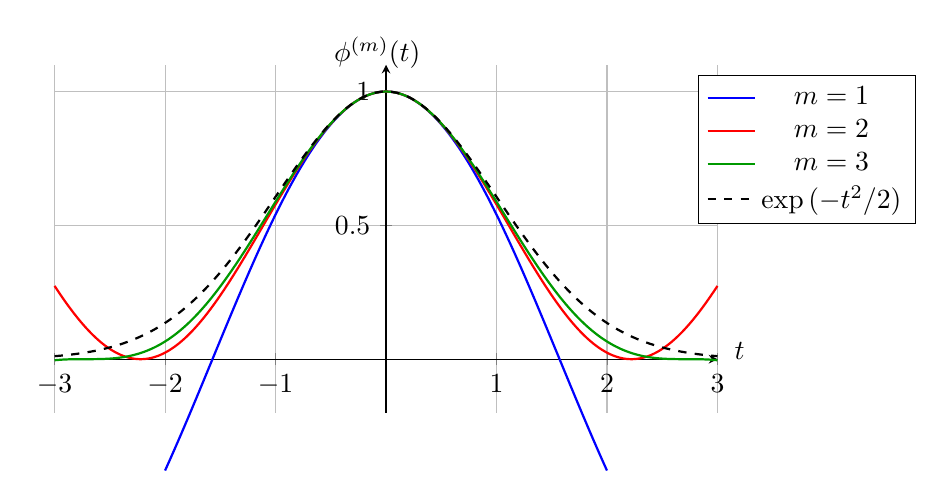
\begin{tikzpicture}
			\begin{axis}[
			width=10cm,
			height=6cm,
			xlabel={},
			ylabel={},
			legend style={at={(0.97,0.97)}, anchor=north west},
			domain=-3:3,
			ylabel style={
			yshift=10pt   % shift label up by 10pt
			},
			samples=400,
			ymin=-0.2, ymax=1.1,
			axis lines=middle,
			clip=false,
			grid=both,
			]
			\addplot[thick, blue,domain=-2:2] {cos(x/sqrt(1) r)^1};
			\addlegendentry{$m=1$}
			\addplot[thick, red] {cos(x/sqrt(2) r)^2};
			\addlegendentry{$m=2$}
			\addplot[thick, green!60!black] {cos(x/sqrt(3) r)^3};
			\addlegendentry{$m=3$}
			\addplot[thick, dashed, black] {exp(-x^2/2)};
			\addlegendentry{$\exp\,(-t^2/2)$}
			\node[anchor=south, rotate=0] at (axis cs:-0.08,1.05) {$\phi^{(m)}(t)$};
			\node[anchor=north, rotate=0] at (axis cs: 3.2,0.1) {$t$};
			\end{axis}
			\end{tikzpicture}
			\caption{Characteristic functions of normalized sums of independent and identically distributed (i.i.d.) random variables (RVs) $x^{(r)} \in \{-1,1\}$ 
			for $r=1,\,\ldots,\,m$ compared to the Gaussian limit.}
		\end{figure}
		See also: random variable (RV), Gaussian random variable (Gaussian RV).},
	first={central limit theorem (CLT)},
	type=math, 
	text={CLT}
}

\newglossaryentry{indicatorfunc}
{name={indicator function}, 
  description={Consider some process\index{indicator function} that can result in different possible 
                outcomes (e.g., survival or death of a patient). Such 
				a process can be modeled as a random experiment with 
				sample space $\Omega$ containing all possible outcomes. 
				The indicator function $\mathbb{I}_{\mathcal{C}}$ of an event 
				$\mathcal{C}\subseteq \Omega$ is a function defined as \cite{BertsekasProb} 
				\[\mathbb{I}_{\mathcal{C}}(\omega) = \begin{cases}
					1, & \text{if } \omega\in \mathcal{C}, \\
					0, & \text{if } \omega\notin \mathcal{C}.
					\end{cases}
				\]
				The notion of an indicator function is not limited to outcomes of 
				a random experiment. Utlimately it is just a principled way to 
				to represent a set $\mathcal{C}$ by a functions $\mathbb{I}_{\mathcal{C}}$ \cite{BoydConvexBook}.}, 
  first={indicator function},
  plural={indicator functions}, 
  type=math, 
  text={indicator function}
}

\newglossaryentry{probmodel}
{name={probabilistic model}, 
	description={A probabilistic model\index{probabilistic model} for the 
				  generation of data points consists of random variables (RVs) 
				  with a joint probability distribution \cite{BertsekasProb}. 
				  This joint probability distribution typically involves parameters (or model parameters) 
				  that are either chosen manually or learned via statistical inference 
				  methods such as maximum likelihood estimation \cite{LC}.
					\\ 
		See also: model, data point, random variable (RV), probability distribution, parameter, maximum likelihood, realization. }, 
	first={probabilistic model}, 
	plural={probabilistic models},
	firstplural={probabilistic models},
	type=math,
	text={probabilistic model} 
}

\newglossaryentry{mean}
{name={mean}, plural={means},
	description={The\index{mean} mean of an random variable (RV) ${\bf x}$, which takes 
 		on values in a Euclidean space $\mathbb{R}^{d}$, is its 
 		expectation $\mathbb{E} \{{\bf x}\}$. It is defined as the Lebesgue 
 		integral of ${\bf x}$ with respect to the underlying probability distribution $P$ (e.g., 
		see \cite{RudinBookPrinciplesMatheAnalysis} or \cite{BillingsleyProbMeasure}), i.e.,
		\[
			\mathbb{E} \{{\bf x}\} = \int_{\mathbb{R}^{d}} {\bf x}\, \mathrm{d}P({\bf x}).
		\]  
		We also use the term to refer to the average of a finite dataset
		$\mathcal{D}= \left\{ {\bf x}^{(1)}, \,\ldots, \,{\bf x}^{(m)} \in \mathbb{R}^{d}\right\}$. 
		However, these two definitions are essentially the same. Indeed, we can use 
		a dataset to construct a discrete random variable (RV) $\widetilde{{\bf x}}^{(\mathcal{D})}={\bf x}^{(I)}$ on 
		the sample space $\{1, \,\ldots, \,m\}$. Here, the index $I$ is 
		chosen uniformly at random, $\mathbb{P}\left(I=r\right)=1/m$ for all 
		$r=1,\ldots,m$. The mean of $\widetilde{{\bf x}}^{(\mathcal{D})}$ is 
		precisely the average $({1}/{m}) \sum_{r=1}^{m} {\bf x}^{(r)}$.
		For an random variable (RV) with finite second-order moment, i.e., 
		$\mathbb{E} \{ \mleft\lVert {\bf x}\mright\rVert_{2}^{2} \}$ is well-defined and fnite, 
		the mean is characterized as the solution of the 
		following risk minimization problem \cite{BertsekasProb}:
		\[
			\mathbb{E} \{{\bf x}\} = \argmin_{{\bf c}\in \mathbb{R}^{d}} 
			\mathbb{E} \big\{\mleft\lVert {\bf x}- {\bf c}\mright\rVert_{2}^{2}\big \}.
		\]
		For the random variable (RV) $\widetilde{{\bf x}}^{(\mathcal{D})}$, associated with a dataset, 
		this optimization problem reduces to empirical risk minimization (ERM) with squared error loss on $\mathcal{D}$. 
		\\ 
		See also: random variable (RV), expectation, probability distribution, empirical risk minimization (ERM).}, 
	first={mean}, 
	type=math,
	text={mean} 
}

\newglossaryentry{median}
{name={median}, 
plural={medians},
	description={A\index{median} median $\mathrm{med}\,(x)$ of a real-valued random variable (RV) $x$ 
 		is any number $M \in \mathbb{R}$ such that $\mathbb{P}\left( x \leq M\right) \geq 1/2$ and 
		$\mathbb{P}\left( x \geq M\right) \geq 1/2$ 
		(see Fig. \ref{fig_median1_dict}) \cite{LC}. 
 		\begin{figure}[H]
			\begin{center}
			\begin{tikzpicture}
 			\begin{axis}[
    			axis lines=middle,
    			xlabel={},
    			ylabel={},
    			ymin=0, ymax=1.1,
    			xmin=-2, xmax=6,
    			xtick=\empty,
    			ytick={0,1/2,1},
    			domain=-2:6,
    			samples=200,
    			width=10cm,
    			height=6cm,
    			smooth,
    			enlargelimits=true,
    			clip=false
  			]
    			% Shifted sigmoid CDF
			\addplot[thick, blue, name path=cdf] {1/(1 + exp(-(x - 1)))} node[pos=0.5, above, yshift=15pt] {$\mathbb{P}\left(x \leq \eta\right)$};    % Vertical and horizontal ruler at F(x) = 0.5
    			\draw[dashed, gray] (axis cs:1,0) -- (axis cs:1,0.5); % vertical
    			\draw[dashed, gray] (axis cs:-2,0.5) -- (axis cs:1,0.5); % horizontal
    			% Mark the median point
   			\filldraw[red] (axis cs:1,0.5) circle (2pt);
  		    	\node[below] at (axis cs:1,0) {$M$};
			\node[above right] at (axis cs:6.3,0) {$\eta$};
    			% Label next to curve
  			\end{axis}
			\end{tikzpicture} 
			\end{center}
		\caption{The median of a real-valued random variable (RV) is any number $M$ 
			that partitions $\mathbb{R}$ into two rays with equal probability. \label{fig_median1_dict}}
 		\end{figure}  
 		We can define the median $\mathrm{med}\,(\mathcal{D})$ 
 		of a dataset $\mathcal{D}= \{ x^{(1)}, \,\ldots, \,x^{(m)} \in \mathbb{R} \}$ 
 		via a specific random variable (RV) $\tilde{x}^{(\mathcal{D})}$ that is naturally associated with $\mathcal{D}$. 
 		In particular, this random variable (RV) is defined on the sample space $\{1, \,\ldots, \,m\}$ 
		via $\tilde{x}^{(\mathcal{D})} :=x^{(I)}$. Here, the index $I$ is chosen uniformly 
		at random, i.e., $\mathbb{P}\left(I = r\right)=1/m$ for 
 		all $r=1, \,\ldots, \,m$. If the random variable (RV) $x$ is integrable, any 
		median of $x$ solves the optimization problem: 
 		$$\min_{x' \in \mathbb{R}} \mathbb{E} {|x - x'|}.$$ 
		For a the above random variable (RV) $\tilde{x}$ (constructed from a dataset $\mathcal{D}$), 
		this optimization problem is empirical risk minimization (ERM) on $\mathcal{D}$ using absolute error loss. 
 		Like the mean, the median of a dataset $\mathcal{D}$ can also be used 
 		to estimate parameters of an underlying probabilistic model. Compared 
 		with the mean, the median is more robust to outliers. For example, 
 		a median of a dataset $\mathcal{D}$ with more than one data point does not 
 		change even if we arbitrarily increase the largest element of $\mathcal{D}$ (see Fig. \ref{fig_median2_dict}). 
		In contrast, the mean will increase arbitrarily.
		\begin{figure}[H]
		\centering
		\begin{tikzpicture}[scale=0.7, y=0.5cm, x=0.5cm]
			\begin{scope}
				\foreach \x/\y in {
					1/2, 4/3, 7/4
				} {
					\draw[dashed, gray] (\x, 0) -- (\x, \y);
					\filldraw[blue] (\x, \y) circle (2pt);
					\node[circle, inner sep=0pt] (ptA\x) at (\x, \y) {};
				}
				\draw[dashed, thick] (0.5, 3) -- (10.5, 3) node[right] {$\mathrm{med}\,(\mathcal{D})\!=\!{\rm mean}(\mathcal{D})$};
				\node at (7.5, -4) {(a)};
			\end{scope}
			\begin{scope}[xshift=12cm]
				\foreach \x/\y in {
					1/2, 4/3, 7/10
				} {
					\draw[dashed, gray] (\x, 0) -- (\x, \y);
					\filldraw[blue] (\x, \y) circle (2pt);
					\node[circle, inner sep=0pt] (ptB\x) at (\x, \y) {};
				}
				\draw[dashed, thick] (0.5, 7.5) -- (10.5, 7.5) node[right] 
				{${\rm mean}\,\big(\widetilde{\mathcal{D}}\big)$};
				\draw[dashed, thick] (0.5, 3) -- (10.5, 3) node[right] 
				{$\mathrm{med}\,\big(\widetilde{\mathcal{D}}\big)$};
				\node[above right=2pt and 2pt, red] at (ptB7) {outlier};
				\node at (7.5, -4) {(b)};
			\end{scope}
		\end{tikzpicture}
		\caption{The median is robust against outlier contamination. (a) Original dataset $\mathcal{D}$. (b) Noisy 
			dataset $\widetilde{\mathcal{D}}$ including an outlier. \label{fig_median2_dict}}
		\end{figure}
		See also: mean, outlier, robustness, least absolute deviation regression.}, 
	first={median}, 
	type=math,
	text={median} 
}

\newglossaryentry{variance}
{name={variance},
	description={The\index{variance} variance of a real-valued random variable (RV) $x$ is defined 
	   	as the expectation $\mathbb{E} \big\{ \big( x - \mathbb{E} \{x \} \big)^{2} \big\}$ of 
	   	the squared difference between $x$ and its expectation $\mathbb{E} \{x \}$. 
	   	We extend this definition to vector-valued random variables (RVs) ${\bf x}$ 
	   	as $\mathbb{E} \big\{ \big\| {\bf x}- \mathbb{E} \{{\bf x}\} \big\|_{2}^{2} \big\} = {\rm tr} \left(\mathbf{C}^{({\bf x})}\right)$,
          	i.e., the sum of the variances of each entry of ${\bf x}$, which can be written compactly 
		as the trace of the covariance matrix $\mathbf{C}^{({\bf x})}$ of ${\bf x}$. 
          	\\ 	 
		See also: random variable (RV), expectation, vector.},
	first={variance},
	type=math,
	text={variance} 
}

\newglossaryentry{probabilitysimplex}
{name={probability simplex},
	description={The\index{probability simplex} probability simplex
   		$\Delta^{k-1}$ is the set of all vectors 
   		in $\mathbb{R}^k$ with nonnegative entries 
 		that sum to one \cite{BoydConvexBook}. Each element of $\Delta^{k-1}$ 
		represents a probability mass function (pmf) of an random variable (RV) $y \in \{1,\,\ldots,\,k\}$.
		\\
		See also: probability, vector, probability mass function (pmf), random variable (RV). },
  	first={probability simplex},
  	plural={probability simplexes},
  	firstplural={probability simplexes},
  	type=math,
  	text={probability simplex}
}

\newglossaryentry{projection}
{name={projection}, 
       	description={Consider\index{projection} a bounded subset 
		$\mathcal{W}\subseteq \mathbb{R}^{d}$ of 
		the $d$-dimensional Euclidean space. We define the projection 
		$P_{\mathcal{W}}\big( {\bf w}\big) $ of a vector 
		${\bf w}\in \mathbb{R}^{d}$ onto $\mathcal{W}$ as
	   	\begin{equation} 
   	   		\nonumber
			\label{equ_def_proj_generic_dict}
  	    		P_{\mathcal{W}}\big( {\bf w}\big)  = \argmin_{{\bf w}' \in \mathcal{W}} \mleft\lVert {\bf w}- {\bf w}' \mright\rVert_{2}. 
        	    	\end{equation}
	    	In other words, $P_{\mathcal{W}}\big( {\bf w}\big) $ is the vector in $\mathcal{W}$ 
	    	that is closest to ${\bf w}$. The projection is only well defined for subsets $\mathcal{W}$ 
	    	for which the above minimum exists \cite{BoydConvexBook}.
		 			\\ 
	    	See also: Euclidean space, vector, minimum.},
	first={projection},
	type=math,
	text={projection}
}

\newglossaryentry{projgd}
{name={projected gradient descent (projected GD)},
	description={Consider an empirical risk minimization (ERM)-based method that uses a parameterized model with  
		parameter space $\mathcal{W}\subseteq \mathbb{R}^{d}$. Even if 
		the objective function of empirical risk minimization (ERM) is smooth, we cannot use basic gradient descent (GD), as 
		it does not take into account constraints on the optimization variable (i.e., the model parameters). 
		Projected\index{projected gradient descent (projected GD)} gradient descent (GD) 
		extends basic gradient descent (GD) to address this issue. 
		A single iteration of projected gradient descent (GD) consists of first taking a gradient step 
		and then projecting the result back onto the parameter space. 
		See Fig. \ref{fig_projected_GD_dict} for a visual illustration.
		\begin{figure}[H]
		\begin{center}
			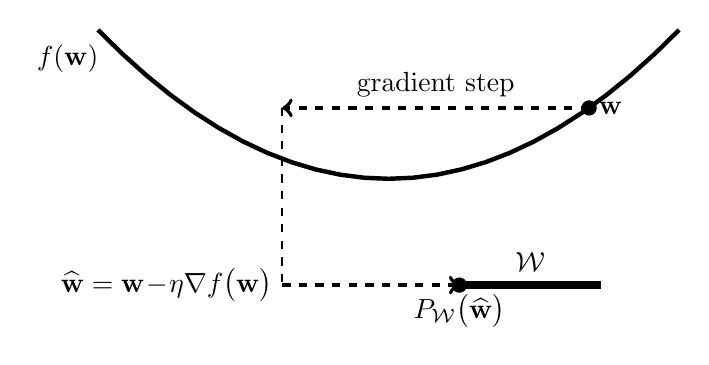
\begin{tikzpicture}[scale=0.9]
			\node [right] at (-5.1,1.7) {$f({\bf w})$} ;
			\draw[ultra thick, domain=-4.1:4.1] plot (\x,  {(1/8)*\x*\x});
		%	\draw[dashed, thick, domain=1:3.6] plot (\x,  {\x - 1}) node[right] {$ f\big(\weights^{(\itercntr)}\big)\!+\!\big(\weights\!-\!\weights^{(\itercntr)}\big)^{T} \nabla f\big(\weights^{(\itercntr)}\big)$};
			\draw [fill] (2.83,1) circle [radius=0.1] node[right] {${\bf w}$};
			\draw[line width =0.5mm,dashed,->] (2.83,1) -- node[midway,above] {gradient step} (-1.5,1);
			\draw[line width =0.2mm,dashed] (-1.5,1) --(-1.5,-1.5)  node [below, left]{$\widehat{{\bf w}}={\bf w}\!-\!\eta\nabla f\big({\bf w}\big)$} ;
			\draw[line width =0.5mm,dashed,->] (-1.5,-1.5)  -- node[midway,above] {} (1,-1.5) ; 
			\draw [fill] (1,-1.5) circle [radius=0.1] node[below] {$P_{\mathcal{W}}\big( \widehat{{\bf w}}\big) $};
			\draw[line width=1mm] (1,-1.5) -- (3,-1.5) node[midway, above] {$\mathcal{W}$};
			\end{tikzpicture}
		\vspace*{-5mm}
		\end{center}
		\caption{Projected gradient descent (GD) augments a basic gradient step with a projection back 
			onto the constraint set $\mathcal{W}$.}
			\label{fig_projected_GD_dict}
		\end{figure}
		See also: empirical risk minimization (ERM), model, parameter space, objective function, smooth, gradient descent (GD), model parameter, gradient step, projection.},
	first={projected gradient descent (projected GD)},
	type=math, 
	text={projected GD}
}

\newglossaryentry{proximable}
{name={proximable},
	description={A\index{proximable} 
		convex function for which the proximal operator can be computed efficiently is 
		sometimes referred to as proximable or simple \cite{Condat2013}.
					\\ 
		See also: convex, function, proximal operator.},
	first={proximable},
	type=math,
	text={proximable}
}

\newglossaryentry{operator} 
{name={operator}, 
	description={An\index{operator} operator is a function 
		whose domain and co-domain have a specific 
		mathematical structure such as a vector space, a Hilbert space,
		or a metric space \cite{Bauschke:2017}, \cite{DunfordSchwartz1988}. 
		Many machine learning (ML) methods involve operators whose domain and co-domain 
		are Euclidean spaces.
							\\ 
		See also: function, vector space, Hilbert space.},
	first={operator},
	type=math, 
	plural={operators},
	firstplural={operators},
	text={operator}
}

\newglossaryentry{ergraph}
{name={Erd\H{o}s–R\'enyi graph (ER graph)},
	description={An ER graph\index{Erd\H{o}s–R\'enyi graph (ER graph)} \cite{erdds1959random}, \cite{gilbert1959random} 
            	is a probabilistic model for graphs defined over a given node set $i=1, \,\ldots, \,n$. 
            	One way to define the ER graph is via the collection of independent and identically distributed (i.i.d.) binary 
            	random variables (RVs) $b^{(\{i,i'\})} \in \{0,1\}$, 
		for each pair of different nodes $i, i'$. A specific realization  
		of an ER graph contains an edge $\{i,i'\}$ if and only if 
		$b^{(\{i,i'\})}=1$. The ER graph is parameterized by the 
		number $n$ of nodes and the probability $\mathbb{P}\left(b^{(\{i,i'\})}=1\right)$.	
		\\
		See also: graph, probabilistic model, independent and identically distributed (i.i.d.), random variable (RV), realization, probability.},
	first={Erd\H{o}s–R\'enyi graph (ER graph)},
	type=math,
	text={ER graph}
}

\newglossaryentry{condprobdist}
{name={conditional probability distribution}, 
	description={Consider\index{conditional probability distribution} 
     		a stochastic process consisting of two random variables (RVs) ${\bf x}$ and $y$ 
    		with probability distribution $\mathbb{P}^{({\bf x},y)}$. The conditional 
    		probability distribution of $y$ given (or conditioned on) ${\bf x}$ is 
    		denoted by $\mathbb{P}^{(y\mid{\bf x})}$. It is defined via the 
    		conditional expectations of the indicator functions of  
    		measurable sets in the $\sigma$-algebra generated by 
    		the random variable (RV) $y$ \cite{BillingsleyProbMeasure}, \cite{KallenbergBook}.
		\\
		See also: probability distribution, conditional expectation. },
  	first={conditional probability distribution}, 
  	plural={conditional probability distributions},
  	type=math, 
  	text={conditional probability distribution}
}

\newglossaryentry{linearmap}
{name={linear map}, plural={linear maps}, 
	description={A\index{linear map} linear map 
		$f: \mathbb{R}^d\rightarrow \mathbb{R}^m$ 
	    	is a function that satisfies additivity, i.e.,
		$f({\bf x}+ {\bf y}) = f({\bf x}) + f({\bf y})$, and homogeneity, i.e.,
		$f(c{\bf x}) = c f({\bf x})$, for all vectors ${\bf x}, {\bf y}\in \mathbb{R}^d$ 
		and scalars $c \in \mathbb{R}$. In particular, $f(\mathbf{0}) = \mathbf{0}$. 
		Any linear map can be represented as a matrix multiplication 
		$f({\bf x}) = {\bf A}{\bf x}$, for some matrix ${\bf A}\in \mathbb{R}^{m \times n}$. 
		The collection of real-valued linear maps (where $m=1$), 
		for a given dimension $d$, constitute a linear model. The notion 
		of a linear map can be generalized from the domain $\mathbb{R}^{d}$ 
		and co-domain $\mathbb{R}^{m}$ to arbitrary vector spaces.
		\\
		See also: map, function, vector, matrix, linear model.},
	first={linear map},
	type=math, 
	plural={linear maps}, 
	firstplural={linear maps}, 
	text={linear map}
}

\newglossaryentry{vector}
{name={vector},
	description={A\index{vector} vector is an element of a vector space. 
		In the context of machine learning (ML), a particularly important example of a vector space 
		is the Euclidean space $\mathbb{R}^{d}$, where $d\in \mathbb{N}$ 
		is the (finite) dimension of the space. A vector ${\bf x}\in \mathbb{R}^{d}$ 
		can be represented as a list or one-dimensional (1-D) array of real numbers, i.e., 
		$x_1, \,\ldots, \,x_{d}$ with $x_j\in \mathbb{R}$ for 
		$j= 1, \,\ldots, \,d$. The value $x_j$ is the $j$th 
		entry of the vector ${\bf x}$. It can also be useful to view a vector ${\bf x}\in \mathbb{R}^{d}$ 
		as a function that maps each index $j\in \{1, \,\ldots, \,d\}$ 
		to a value $x_j\in \mathbb{R}$, i.e., ${\bf x}: j\mapsto x_j$. 
		This perspective is particularly useful for the study of kernel methods. See Fig. 
		\ref{fig:vector-function-dual_dict} for the two views of a vector.
		\begin{figure}[H]
			% Left: Stem plot
			\begin{minipage}[c]{0.48\textwidth}
				\centering 
				2, --1, 3, 0, --2, 1
				\begin{minipage}{\textwidth}
				\vspace{5ex}
				\centering
				{\selectfont (a)}
				\end{minipage}
			\end{minipage}
			\hfill
			% Right: Column vector
			\begin{minipage}{0.48\textwidth}
			\centering
			\begin{tikzpicture}
			\begin{axis}[
    				width=6.5cm,
    				height=5cm,
    				title={},
    				xlabel={index $j$},
    				ylabel={$x_j$},
   		 		ymin=-3.5, ymax=3.5,
    				xmin=0.5, xmax=6.5,
   	 			xtick={1,2,3,4,5,6},
    				ytick={-3,-2,-1,0,1,2,3},
    				axis x line=bottom,        % <-- horizontal axis at y=0
    				axis y line=left,          % <-- vertical axis on the left
    				grid=both,
    				major grid style={dotted, gray!60},
    				enlargelimits=0.1
			]
			\addplot+[ycomb, thick, mark=*]
    			coordinates {
        				(1,2)
        				(2,-1)
       	 			(3,3)
        				(4,0)
        				(5,-2)
        				(6,1)
    			};
			\end{axis}
			\node at (2,-2.5) {(b)};
			\end{tikzpicture}
			\end{minipage}
		\caption{Two equivalent views of a vector ${\bf x}= \big( 2, -1, 3, 0, -2, 1 \big)^{T} \in \mathbb{R}^{6}$.
			(a) As a numeric array. (b) As a map $j\mapsto x_j$.}
			\label{fig:vector-function-dual_dict}
		\end{figure}
		See also: vector space, Euclidean space, linear map.},
	first={vector},
	firstplural={vectors},
	type=math,
	plural={vectors},
	text={vector}
}

\newglossaryentry{vectorspace}
{name={vector space},
	description={A\index{vector space} vector space $\mathcal{V}$ (also called linear space) 
		is a collection of elements, called vectors, along with the following two operations 
		(see also Fig. \ref{fig:vector-ops_dict}): 
    		1) addition (denoted by ${\bf v}+{\bf w}$) of two vectors ${\bf v},{\bf w}$; and 2) multiplication 
		(denoted by $c \,\cdot \,{\bf v}$) of a vector ${\bf v}$ with a scalar $c$ that belongs to some 
		number field (such as the real numbers $\mathbb{R}$ or the complex numbers $\mathbb{C}$). The defining 
		property of a vector space is that it is closed under two specific operations. First, 
		if ${\bf v}, {\bf w}\in \mathcal{V}$, then ${\bf v}+ {\bf w}\in \mathcal{V}$. Second, if ${\bf v}\in \mathcal{V}$ 
		and $c \in \mathbb{R}$, then $c {\bf v}\in \mathcal{V}$.
		\begin{figure}[H]
		\centering
			\begin{tikzpicture}[>=Stealth, scale=1.2]
			% Coordinates
  			\coordinate (O) at (0,0);            % Origin
  			\coordinate (V) at (2,1.5);          % vector v
  			\coordinate (W) at (1,3);            % vector w
  			\coordinate (VplusW) at (3,4.5);     % v + w
  			\coordinate (HalfV) at (1,0.75);     % 0.5 * v
  			\draw[->, thick, blue] (O) -- (V) node[pos=1, right] {${\bf v}$};
  			\draw[->, thick, red] (O) -- (W) node[pos=1, left] {${\bf w}$};
  			\draw[->, thick, purple] (O) -- (VplusW) node[pos=0.99, above right] {${\bf v}+{\bf w}$};
  			\draw[dashed, red] (V) -- (VplusW);
  			\draw[dashed, blue] (W) -- (VplusW);
  			\draw[->, thick, orange] (O) -- (HalfV) node[midway, right] {$ \alpha {\bf v}$};
			% Filled dots
  			\filldraw[black] (O) circle (2pt) node[below left] {$\mathbf{0}$};  % origin
  			\filldraw[blue] (V) circle (2pt);         % v
  			\filldraw[red] (W) circle (2pt);          % w
  			\filldraw[purple] (VplusW) circle (2pt);  % v + w
  			\filldraw[orange] (HalfV) circle (2pt);   % 0.5v
			\end{tikzpicture}
			\caption{A vector space $\mathcal{V}$ is a collection of vectors such that 
			scaling and adding them always yields another vector in $\mathcal{V}$.}
			%In \gls{ml}, we use vector spaces to represent \glspl{rv}, \glspl{datapoint} 
			%(or their \glspl{featurevec}) as well as invariances (or symmetries) of \glspl{model}.}
			\label{fig:vector-ops_dict}
		\end{figure}
		A common example of a vector space is the Euclidean space $\mathbb{R}^n$, which is 
		widely used in machine learning (ML) to represent datasets. We can also use $\mathbb{R}^n$ 
		to represent, either exactly or approximately, the hypothesis space used by an machine learning (ML) method.  
		Another example of a vector space, which is naturally associated with every probability space 
		$\big(\Omega,\mathcal{F},\mathbb{P}\left(\cdot\right) \big)$, is the collection of all 
		real-valued random variables (RVs) $x: \Omega\rightarrow \mathbb{R}$ \cite{RudinBook}, \cite{folland1999real}.  
		\\
		See also: vector, Euclidean space, linear model, linear map.},
	first={vector space},
	plural={vector spaces}, 
	firstplural={vector spaces}, 
	type=math,
	text={vector space}
}

\newglossaryentry{stochastic}
{name={stochastic},
	description={We refer to a\index{stochastic} method as stochastic if it involves a 
		random component or is governed by probabilistic laws. Machine learning (ML) methods use randomness 
		to reduce computational complexity (e.g., see stochastic gradient descent (SGD)) or 
		to capture uncertainty in probabilistic models.
		\\
		See also: stochastic gradient descent (SGD), uncertainty, probabilistic model.},
	first={stochastic},
	type=math, 
	text={stochastic}
}

\newglossaryentry{stochproc}
{name={stochastic process},
	description={A stochastic process\index{stochastic process} is a collection of 
		random variables (RVs) defined on a common probability space and indexed by some set 
		$\mathcal{I}$ \cite{GrayProbBook}, \cite{papoulis}, \cite{Brockwell91}. The index set 
		$\mathcal{I}$ typically represents time or space, allowing us to represent 
		random phenomena that evolve across time or spatial dimensions—for example, 
		sensor noise or financial time series. Stochastic processes are not limited 
		to temporal or spatial settings. For instance, random graphs such as 
		the Erd\H{o}s–R\'enyi graph (ER graph) or the stochastic block model (SBM) can also be viewed as stochastic processes. 
		Here, the index set $\mathcal{I}$ consists of node pairs that index random variables (RVs) whose values 
		encode the presence or weight of an edge between two nodes. Moreover, stochastic 
		processes naturally arise in the analysis of stochastic algorithms, 
		such as stochastic gradient descent (SGD), which construct a sequence of random variables (RVs). 
		\\
		See also:  random variable (RV), stochastic block model (SBM), stochastic gradient descent (SGD), uncertainty, probabilistic model.},
	first={stochastic process},
	firstplural={stochastic processes},
	type=math, 
	plural={stochastic processes},
	text={stochastic process}
}

\newglossaryentry{characteristicfunc}
{name={characteristic function},
	description={The characteristic function\index{characteristic function} 
		of a real-valued random variable (RV) $x$ is the function \cite[Sec. 26]{BillingsleyProbMeasure}
		$$ \phi_{x}(t) :=\mathbb{E} { \exp\,(j t x) } \mbox{ with } j = \sqrt{-1}.$$
	 	The characteristic function uniquely determines the probability distribution of $x$. 
		\\
		See also: random variable (RV), probability distribution.},
	first={characteristic function},
	firstplural={characteristic functions}, 
	type=math, 
	plural={characteristic functions},
	text={characteristic function}
}

\newglossaryentry{entropy}
{name={entropy},
	description={Entropy\index{entropy} quantifies the uncertainty or 
		unpredictability associated with an random variable (RV) \cite{coverthomas}. 
		For a discrete random variable (discrete RV) $x$ taking on values in a finite set 
		$\mathcal{S} = \{x_1, \,\ldots, \,x_k\}$ with 
		a probability mass function (pmf) $p^{(x)}\left(x_{c}\right) (=\mathbb{P}\left(x = x_{c}\right))$, 
		the entropy is defined as \cite{coverthomas}
		\[
		   H\left(x\right) :=-\sum_{c=1}^{k} p^{(x)}\left(x_{c}\right)  \log p^{(x)}\left(x_{c}\right) .
		\]
		For a given set of values $\mathcal{S}$, the entropy is maximized for a 
		uniformly distributed random variable (RV), where $p^{(x)}\left(x_{c}\right)=1/k$. 
		The minimal entropy, which is zero, is obtained when $p^{(x)}\left(x_{c}\right)=1$ 
		for some $x_{c} \in \mathcal{S}$.
		Differential entropy generalizes the concept of entropy from discrete random variables (discrete RVs) to 
		continuous random variables (RVs). 
		\\
		See also: uncertainty, probabilistic model.},
	first={entropy},
	type=math, 
	text={entropy}
}

\newglossaryentry{diffentropy}
{name={differential entropy},
	description={For\index{differential entropy} an 
		random variable (RV) ${\bf x}\in \mathbb{R}^{d}$ 
		with a probability density function (pdf) $p^{(x)}\left(\cdot\right)$, the differential entropy 
		is defined as \cite{coverthomas}
		\[
		h({\bf x}) :=- \int_{{\bf x}' \in \mathbb{R}^{d}} 
            %\log p(\featurevec') \, d \pdf{\featurevec}{\featurevec'} .
		\log p({\bf x}') p^{({\bf x})}\left({\bf x}'\right) \, d {\bf x}'.
            \]
		Differential entropy can be negative and lacks some properties of 
		entropy for discrete-valued random variables (RVs), such as invariance under 
		a change of variables \cite{coverthomas}. Among all random variables (RVs) with a 
		given mean ${\bm \mu}$ and covariance matrix ${\bf C}$, 
		$h({\bf x})$ is maximized by ${\bf x}\sim \mathcal{N}\left({\bm \mu},{\bf C}\right)$. 
		\\
		See also: uncertainty, probabilistic model.},
	first={differential entropy},
	type=math,
	text={differential entropy}
}

\newglossaryentry{domain}
{name={domain}, 
	description={The domain\index{domain} of a function 
		$f: \mathcal{U} \rightarrow \mathcal{V}$ is the set $\mathcal{U}$ 
		from which $f$ takes its inputs.  
		\\
		See also: function, co-domain, map.},
	first={domain},
	firstplural={domains}, 
	type=math, 
	plural={domains},
	text={domain}
}

\newglossaryentry{function}
{name={function}, 
	description={A function\index{function} between two sets $\mathcal{U}$ and $\mathcal{V}$ assigns  
		each element $u \in \mathcal{U}$ exactly one element $f(u) \in \mathcal{V}$ \cite{RudinBookPrinciplesMatheAnalysis}.
		We write this as $$f: \mathcal{U} \rightarrow \mathcal{V}: u \mapsto f(u)$$ 
		where $\mathcal{U}$ is the domain and $\mathcal{V}$ the co-domain of $f$. 
		That is, a function $f$ defines a unique output $f(u) \in \mathcal{V}$ for every 
		input $u \in \mathcal{U}$ (see Fig. \ref{fig_function_dict}).
		\begin{figure}[H]
			\centering
			\begin{tikzpicture}[>=stealth, node distance=1.2cm and 2.5cm]
				\tikzset{dot/.style={circle, fill=black, inner sep=1.2pt}}
				\node (A) [dot, label=left:$a$] {};
				\node (B) [dot, below=of A, label=left:$b$] {};
				\node (C) [dot, below=of B, label=left:$c$] {};
				\node (1) [dot, right=4cm of A, label=right:$\star$] {};
				\node (2) [dot, below=of 1, label=right:$\circ$] {};
				\node (3) [dot, below=of 2, label=right:$\otimes$] {};
				\node[draw=blue!70, thick, ellipse, inner sep=0.5cm, fit=(A)(B)(C), label=above:$\mathcal{U}$] {};
				\node[draw=green!70!black, thick, ellipse, inner sep=0.5cm, fit=(1)(2)(3), label=above:$\mathcal{V}$] {};
				\draw[->] (A) -- (2);
				\draw[->] (B) -- (1);
				\draw[->] (C) -- (2);
			\end{tikzpicture}
			\caption{A function \( f \colon \mathcal{U} \to \mathcal{V} \) mapping each element 
				of the domain $\mathcal{U} =  \{a,b,c\}$ to exactly one element of 
				the co-domain $\mathcal{V} = \{\star,\circ,\otimes\}$. \label{fig_function_dict}}
		\end{figure} 
		See also: domain, co-domain, output. },
	first={function},
	firstplural={functions}, 
	type=math, 
	plural={functions},
	text={function}
}

\newglossaryentry{map}
{name={map}, 
	description={We\index{map} use the term map as a synonym for function.
		\\
		See also: function.},
	first={map},
	firstplural={maps},	
	type=math, 
	plural={maps},
	text={map}
}

\newglossaryentry{event}
{name={event}, 
	description={Consider\index{event} an random variable (RV) ${\bf x}$, defined on some probability space, 
		which takes values in a measurable space $\mathcal{X}$. An 
		event $\mathcal{A} \subseteq \mathcal{X}$ is a subset of $\mathcal{X}$ 
		such that the probability $\mathbb{P}\left({\bf x}\in \mathcal{A}\right)$ is well 
		defined. In other words, the preimage ${\bf x}^{-1}(\mathcal{A})$ 
		of an event belongs to the underlying $\sigma$-algebra, i.e., the preimage 
		is a measurable subset of the sample space 
		\cite{RudinBook}, \cite{BillingsleyProbMeasure}, \cite{durrett2010probability}.	
		Roughly speaking, an event represents a set of possible outcomes of some 
		process. One example of such a process could also be the treatment of a 
		health-care patient.
				\\
		See also: random variable (RV), data point, independent and identically distributed assumption (i.i.d.\ assumption), probabilistic model.},
	first={event},
	firstplural={events},
	plural={events},
	type=math,
	text={event} 
}

\newglossaryentry{countable}
{name={countable},
	description={A set is called countable\index{countable} if its 
		elements can be put into a one-to-one correspondence with the natural numbers 
		$\mathbb{N}=\{1,\,2,\,3,\,\ldots\}$ or with a finite subset of $\mathbb{N}$ \cite{HalmosSet}. 
		Equivalently, a set $\mathcal{A}$ is countable if there exists an injective 
		function $f:\mathcal{A}\rightarrow\mathbb{N}$. 
		\begin{figure}[H]
			\centering
			\begin{tikzpicture}[>=stealth, node distance=1.0cm, thick]
  			%--- Left: elements of set A ---
  			\node (a1) {$a_1$};
  			\node[below=of a1] (a2) {$a_2$};
  			\node[below=of a2] (a3) {$a_3$};
  			\node[left=0.4cm of a2, align=center] {$\mathcal{A}$};
  			% Ellipse enclosing set A
  			\begin{scope}[on background layer]
    			\draw[rounded corners, dashed, gray] ($(a1)+(-0.5,0.4)$) rectangle ($(a3)+(0.5,-0.4)$);
  			\end{scope}
  			%--- Right: natural numbers ---
  			\node[right=3.0cm of a1] (n1) {$1$};
  			\node[below=of n1] (n2) {$2$};
  			\node[below=of n2] (n3) {$3$};
  			\node[below=of n3] (n4) {$4$};
  			\node[below=of n4] (ndots) {$\vdots$};
  			\node[right=0.4cm of n2, align=center] {$\mathbb{N}$};
  			%--- Arrows (injective mapping) ---
  			\draw[->] (a1) -- (n3);
  			\draw[->] (a2) -- (n1);
  			\draw[->] (a3) -- (n4);
			\end{tikzpicture}
		\caption{An injective function that maps the elements of a finite set 
			$\mathcal{A}$ to the natural numbers $\mathbb{N}$, which implies that $\mathcal{A}$ is countable.}
		\end{figure}
		Typical examples include the set of integers $\mathbb{Z}$ and rational 
		numbers $\mathbb{Q}$. In contrast, the set of real numbers $\mathbb{R}$ 
		is not countable, meaning no such one-to-one correspondence with $\mathbb{N}$ exists.
		\\ 
		See also: injective, function.}, 
	first={countable}, 
	type=math, 
	text={countable}
}

\newglossaryentry{pmf}
{name={probability mass function (pmf)}, 
	description={The pmf\index{probability mass function (pmf)} 
		of a discrete random variable (discrete RV) $x$ is a function 
		$p^{(x)}\left(\cdot\right): \mathcal{X}\rightarrow [0,1]$ that assigns to each 
		possible value $x' \in \mathcal{X}$ of the random variable (RV) $x$ 
		the probability $p^{(x)}\left(x'\right) = \mathbb{P}\left(x' = x\right)$ \cite{papoulis}. 
		Fig.\ \ref{fig_pmf_dict} illustrates the pmf of a discrete random variable (discrete RV) $x$. 
		\begin{figure}[H]
			\centering
			\begin{tikzpicture}[>=stealth, thick,y=2cm]
  			\foreach \x/\p in {1/0.3, 4/0.7}{
			% Stem lines
			\draw[gray] (\x,0) -- (\x,\p);
			% Dots at the end of stems
			\fill[blue] (\x,\p) circle (2pt);
			% Labels next to each value
			% \node[anchor=west, blue] at (\x+0.1,\p) {\small $\pmf{\feature}{\cdot}$};
			}
  			\node[anchor=south,align=center] at (1,0.3) {\small $p^{(x)}\left(\star\right)=\frac{3}{10}$};
  			\node[anchor=north] at (1,0) {\small $\star$};
  			\node[anchor=north] at (4,0) {\small $\otimes$};
    			%--- Example datasets (same length, same frequencies, different permutations) ---
  			\node[anchor=west,text width=11cm] at (-1.2,-0.80) {
    			$\mathcal{D}= (\star,\,\star,\,\star,\,\otimes,\,\otimes,\,\otimes,\,\otimes,\,\otimes,\,\otimes,\,\otimes)$
  			};
  			\node[anchor=west,text width=11cm] at (-5.2,1.18) {\small
    			$\mathcal{D}' = (\otimes,\,\star,\,\otimes,\,\star,\,\otimes,\,\otimes,\,\star,\,\otimes,\,\otimes,\,\otimes)$
  			};
  			\node[anchor=west,text width=11cm] at (3.2,1.56) {
    			$\mathcal{D}'' = (\otimes,\,\otimes,\,\otimes,\,\star,\,\otimes,\,\star,\,\otimes,\,\otimes,\,\star,\,\otimes)$
  			};
			\end{tikzpicture}
		\caption{The pmf $p^{(x)}\left(\cdot\right)$ of a discrete random variable (discrete RV) $x$ 
			taking values in the set $\mathcal{X}= \{\star,\otimes\}$. Three datasets 
			are also shown whose relative frequencies of data points match 
			this pmf exactly. Such datasets could arise as realizations of 
			independent and identically distributed (i.i.d.) random variables (RVs) sharing the common pmf $p^{(x)}\left(\cdot\right)$. 
			\label{fig_pmf_dict}}
		\end{figure}
		A pmf always satisfies $\sum_{x' \in \mathcal{X}} p^{(x)}\left(x'\right) = 1$. 
		We can view a pmf as representing a collection of (sufficiently long)  
		datasets. This collection contains any 
		$\mathcal{D}= \{x^{(1)}, \,\ldots, \,x^{(m)}\}$, 
		with the relative frequencies of every value $x' \in \mathcal{X}$ 
		being close to the corresponding pmf value $p^{(x)}\left(x'\right)$, 
		$$ \frac{\big|r\in \{1,\,\ldots,\,m\}: x^{(r)}= x' \big|}
		{m} \approx p^{(x)}\left(x'\right).$$ 
		Note that requiring relative frequencies to be close to the pmf values 
		implies that the empirical entropy of such a dataset is close to the 
		entropy of the pmf $p^{(x)}\left(\cdot\right)$. Information theory refers 
		to the collection of such datasets as the typical set corresponding to the pmf 
		$p^{(x)}\left(\cdot\right)$ \cite{coverthomas}. A main result of information theory states 
		that a dataset generated by independent and identically distributed (i.i.d.) sampling from $p^{(x)}\left(\cdot\right)$ 
		belongs, with high probability, to the typical set with respect to $p^{(x)}\left(\cdot\right)$ \cite[Th. 3.1.2]{coverthomas}.
				\\
		See also: discrete random variable (discrete RV), probability, probability distribution, probabilistic model.},
	first={probability mass function (pmf)},
	firstplural={probability mass functions (pmfs)},
	plural={pmfs},
	type=math,
	text={pmf} 
}

\newglossaryentry{discreteRV}
{name={discrete random variable (discrete RV)}, 
 	description={A\index{discrete random variable (discrete RV)} random variable (RV), i.e., 
		a function that maps the outcomes of a random experiment 
		to elements of a measurable space $\mathcal{X}$, 
		is referred to as discrete if its value space 
		$\mathcal{X}$ countable \cite{BillingsleyProbMeasure}. 
			\\
		See also: random variable (RV), probability, probability distribution.},
 	first={discrete random variable (discrete RV)},
	firstplural={discrete random variables (discrete RVs)}, 
	plural={discrete RVs},
	type=math, 
 	text={discrete RV}  
}

\newglossaryentry{rv}
{name={random variable (RV)}, plural={RVs},
 	description={An RV\index{random variable (RV)} is a function that maps the 
		outcomes of a random experiment to elements of a measurable space 
		\cite{BillingsleyProbMeasure}, \cite{GrayProbBook}. 
 		Mathematically, an RV is a function $x: \Omega\rightarrow \mathcal{X}$ 
		whose domain is the sample space $\Omega$ of a probability space and 
		whose co-domain is a measurable space $\mathcal{X}$. 
 		Different types of RVs include  
 		\begin{itemize} 
 			\item {binary RVs}, which map each outcome to an element of a binary 
			set (e.g., $\{-1,1\}$ or $\{\text{cat}, \text{no cat}\}$); 
			\item {discrete random variables (discrete RVs)}, which take on values in a countable set (which can 
			be finite or countably infinite); 
 			\item {real-valued RVs}, which take on values in the real numbers $\mathbb{R}$;  
 			\item {vector-valued RVs}, which map outcomes to the Euclidean space $\mathbb{R}^{d}$.  
 		\end{itemize} 
 		Probability theory uses the concept of measurable spaces to rigorously define 
 		and study the properties of collections of RVs \cite{BillingsleyProbMeasure}.
			\\
		See also: function, random experiment, sample space, probability space, vector, Euclidean space, probability, measurable.}, 
	first={random variable (RV)},
	firstplural={random variables (RVs)},
	plural={RVs},
	type=math,
	text={RV}  
}

\newglossaryentry{outcome}
{name={outcome}, 
  	description={Outcome is one possible\index{outcome} result of a physical process.  
		Such a process could be the observation of a physical phenomenon,  
		a computation performed by an algorithm, or a random experiment  
		\cite{BillingsleyProbMeasure}.   
		\\
 		See also: sample space.},  
	type=math, 
  	first={outcome}, 
 	firstplural={outcomes},
 	plural={outcomes},
  	text={outcome}
}

\newglossaryentry{probspace}
{name={probability space}, 
 	description={A\index{probability space} probability space is a mathematical 
 		structure that allows us to reason about a random experiment, e.g., 
		the observation of a physical phenomenon. 
 	   	Formally, a probability space $\mathcal{P}$ is a triplet 
		$(\Omega, \mathcal{F}, \mathbb{P}\left(\cdot\right))$ where
 		\begin{itemize} 
 			\item  $\Omega$ is a sample space containing all possible outcomes 
			of a random experiment;
 			\item  $\mathcal{F}$ is a $\sigma$-algebra, i.e., a collection of subsets of 
			$\Omega$ (called events) that satisfies certain closure properties 
			under set operations;
 			\item $\mathbb{P}\left(\cdot\right)$ is a probability distribution, i.e., a function that assigns 
			a probability $\mathbb{P}\left(\mathcal{A}\right) \in [0,1]$ to each event $\mathcal{A} 
			\in \mathcal{F}$. This function must satisfy $\mathbb{P}\left(\Omega\right) = 1$ and 
			$\mathbb{P}\left(\bigcup_{i=1}^{\infty} \mathcal{A}_i\right) = \sum_{i=1}^{\infty} \mathbb{P}\left(\mathcal{A}_i\right)$ 
			for any countable sequence of pairwise disjoint events $\mathcal{A}_1, \,\mathcal{A}_2, \,\ldots$ in $\mathcal{F}$.
 		\end{itemize}
 		Probability spaces provide the foundation of probabilistic models 
		that can be used to study the behavior of machine learning (ML) methods \cite{BillingsleyProbMeasure}, \cite{GrayProbBook}, \cite{ross2013first}.
				\\
		See also: probability, random experiment, sample space, event, probability distribution, function, probabilistic model, machine learning (ML).},  
 	first={probability space}, 
	plural={probability spaces},
	firstplural={probability spaces},
	type=math, 
 	text={probability space}
}

\newglossaryentry{integrable}
{name={integrable},
	description={A measurable function $f\!:\!\Omega\!\to\! \mathbb{R}$ 
		defined on a measure space $(\Omega, \,\Sigma, \,\mu)$ 
		is called integrable\index{integrable} if the Lebesgue integral 
		of its absolute value is finite, i.e.,
		\[
		\int_{\Omega} |f(x)|\,\mathrm{d}\mu < \infty.
		\]
		In this case, the Lebesgue integral $\int_{\Omega} f(x)\,\mathrm{d}\mu$ 
		is well-defined and finite. An random variable (RV) $x$ defined on the sample space 
		of a probability space $(\Omega, \,\Sigma, \,\mathbb{P})$ 
		is integrable if 
		\[
		\mathbb{E} \{|x|\}
		= \int_{\Omega} |x(\omega)|\,\mathrm{d}\mathbb{P}< \infty
		\]
		which ensures that the expectation $\mathbb{E} \{|x|\}$ 
		exists and is finite. 
		\\ 
		See also: measure space, measure.},
	first={integrable},
	type=math, 
	text={integrable}
}

\newglossaryentry{measurespace}
{name={measure space},
	description={A measure space\index{measure space} is a triple $(\Omega, \,\Sigma, \,\mu)$ consisting of 
        		a set $\Omega$, a $\sigma$-algebra $\Sigma$ of subsets 
		of $\Omega$, and a measure $\mu\!:\Sigma\!\to\![0,\infty)$. 
        		The measure $\mu$ assigns a nonnegative number to each measurable 
		set $\mathcal{A} \in \Sigma$, generalizing the 
		notions of length, area, or volume in Euclidean spaces \cite{RudinBookPrinciplesMatheAnalysis}, \cite{HalmosMeasure}. 
		Measure spaces provide the mathematical foundation for the 
		Lebesgue integral or the definition of random variables (RVs) as measurable mappings 
        		between measure spaces.  
        		A probability space is a special case of a measure space 
		where the total measure of the sample space is normalized to one, 
        		i.e., $\mu(\Omega) = 1$. In this case, $\mu$ is called a probability distribution.
		\\ 
		See also: measurable, probability space, probability distribution. },
    	first={measure space},
	plural={measure spaces}, 
	firstplural={measure spaces}, 
	type=math, 
    	text={measure space}
}

\newglossaryentry{measure}
{name={measure},
	description={A measure\index{measure} $\mu$ on a set $\Omega$ equipped with a 
		$\sigma$-algebra $\Sigma$ is a function $\mu: \Sigma\to [0, \infty)$ 
		that assigns a nonnegative value to each measurable set 
		$\mathcal{A} \in \Sigma$ such that 
		\cite{RudinBookPrinciplesMatheAnalysis}, \cite{BillingsleyProbMeasure}, \cite{HalmosMeasure}: 
		1) $\mu(\emptyset) = 0$; and 
		2) for any countable collection $\{\mathcal{A}_i\}_{i=1}^{\infty}$ of 
		pairwise disjoint sets in $\Sigma$,
		\[
		\mu\!\left(\bigcup_{i=1}^{\infty} A_i\right) = \sum_{i=1}^{\infty} \mu(A_i)
		\]
		which is referred to as ``countable additivity''.
		\\
		See also: measurable, countable. },
	first={measure},
	type=math, 
	plural={measures}, 
	firstplural={measures}, 
	text={measure}
}

\newglossaryentry{LebesgueIntegral}
{name={Lebesgue integral},
	description={The Lebesgue integral\index{Lebesgue integral} 
		assigns each integrable function 
		$f: \mathbb{R}^{d} \rightarrow \mathbb{R}$ a number 
		$\int_{{\bf x}} f({\bf x}) d{\bf x}$ 
		that is referred to as the integral of $f$. 
		The integral of $f$ can be interpreted as the volume that 
		is enclosed by the function $f$ in the space 
		$\mathbb{R}^{d+1}$. We can compute it be increasingly 
		accurate approximations by simple functions 
		\cite[Ch. 1]{RudinBook}. 
		\begin{figure}[H]
			\centering
			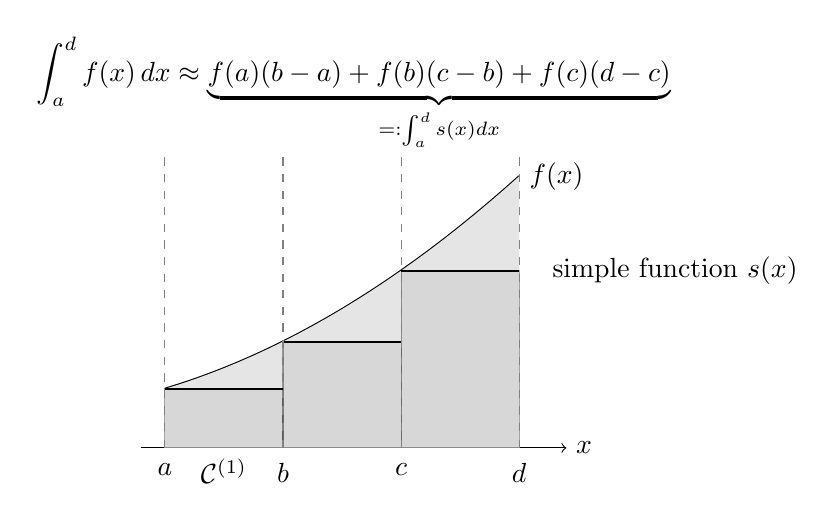
\begin{tikzpicture}[scale=1.5]
  			% Axes
  			\draw[->] (-0.2,0) -- (3.4,0) node[right] {$x$};
 			% \draw[->] (0,-0.1) -- (0,2.6) node[above] {$y$};
  			% Continuous function f(x)
  			\draw[thick,domain=0:3,smooth] plot(\x,{0.5+0.3*\x+0.1*\x*\x}) node[right] {$f(x)$};
  			% Shade area under f(x)
  			\fill[gray!20] (0,0) -- plot[domain=0:3] (\x,{0.5+0.3*\x+0.1*\x*\x}) -- (3,0) -- cycle;
  			% Lower simple function: left-endpoint rectangles for [0,1], [1,2], [2,3]
  			\draw[fill=gray!50,opacity=0.35] (0,0) rectangle (1,0.5);
  			\node at (0.5,-0.2) {$\mathcal{C}^{(1)}$}; 
  			\draw[fill=gray!50,opacity=0.35] (1,0) rectangle (2,0.9);
  			\draw[fill=gray!50,opacity=0.35] (2,0) rectangle (3,1.5);
  			% Step lines of the simple function
  			\draw[thick] (0,0.5)--(1,0.5);
  			\draw[thick] (1,0.9)--(2,0.9);
  			\draw[thick] (2,1.5)--(3,1.5);
 	 		\node[above left] at (0.8,0.5) {};
  			% Dashed partition lines
  			\foreach \x in {0,1,2,3} \draw[dashed,gray] (\x,0) -- (\x,2.5);
  			% Labels
  			\node[anchor=north] at (0,-0.05) {$a$};
  			\node[anchor=north] at (1,-0.05) {$b$};
  			\node[anchor=north] at (2,-0.05) {$c$};
  			\node[anchor=north] at (3,-0.05) {$d$};
  			\node at (1.6,3.0) {$\displaystyle \int_a^d f(x)\,dx \approx \underbrace{f(a)(b-a) + f(b)(c-b)+f(c)(d-c)}_{=:\int_a^d s(x)dx}$};
  			\node [anchor=west] at (3.2,1.5) {simple function $s(x)$};
			\end{tikzpicture}
		\end{figure}
 		It is useful to think of the Lebesgue integral as a function that maps 
 		an integrable function $f$ to the value of its integral, 
		$$ f \mapsto \int_{{\bf x}} f({\bf x}) d{\bf x}.$$ 
		The precise definition of this function, whose domain 
		consists of the integrable functions, is a cornerstone of 
		measure theory \cite[Ch. 1]{RudinBook}.
					\\ 
		See also: function.},
	first={Lebesgue integral},
	text={Lebesgue integral},
	type=math, 
	plural={Lebesgue integrals},
	firstplural={Lebesgue integrals}
}

\newglossaryentry{conditionalexpect}
{name={conditional expectation}, 
	description={Consider a numeric random variable (RV) ${\bf x}\in \mathbb{R}^{d}$ defined on a 
                 probability space $(\Omega,\,\Sigma,\,\mathbb{P})$. 
                 Let $\Sigma' \subseteq \Sigma$ be a (sub-)$\sigma$-algebra that 
                 represents partial information about the outcome of a random experiment. 
                 The conditional expectation\index{conditional expectation} of 
                 ${\bf x}$ given (or conditioned on) $\Sigma'$, denoted 
                 $\mathbb{E} \{ {\bf x}\mid \Sigma'\}$, is a numeric random variable (RV) 
		that \cite{BillingsleyProbMeasure}, \cite{durrett2010probability}:
                	1) is measurable with respect to $\Sigma'$; and
                 2) satisfies
		$$
    		\int_{\mathcal{A}} \mathbb{E} \{{\bf x}\mid \Sigma'\} {\rm d} \mathbb{P}=
    		\int_{\mathcal{A}} {\bf x}{\rm d} \mathbb{P}\quad \text{for any } \mathcal{A} \in \Sigma'.
		$$
               	Intuitively, $\mathbb{E} \{{\bf x}\mid \Sigma'\}$ summarizes 
               	the average value of ${\bf x}$ using only information contained 
               	in the (typically smaller) $\sigma$-algebra $\Sigma'$ 
		\cite{BillingsleyProbMeasure}, \cite{GrayProbBook}, \cite{ross2013first}. 
		\\
              	See also: probability space, $\sigma$-algebra, expectation.}, 
 	first={conditional expectation},
 	plural={conditional expectations}, 
 	type=math, 
 	firstplural={conditional expectations},  
 	text={conditional expectation}
}

\newglossaryentry{conditionalpmf}
{name={conditional probability mass function (conditional pmf)}, 
	description={Consider two discrete random variables (discrete RVs) $y$ and $x$ defined on 
                 the same probability space $(\Omega,\,\mathcal{F},\,\mathbb{P}\left(\cdot\right))$. 
                 The conditional probability mass function (pmf)\index{conditional probability mass function (conditional pmf)} 
                 of $y$ given (or conditioned on) $x$ is denoted by
		$p^{(y\mid x)}\left(\cdot \mid \cdot\right)$ and is defined by
                \[
                  p^{(y\mid x)}\left(y' \mid x'\right)
                  :=
                  \mathbb{P}\left(y=y' \mid x=x'\right)
               \]
                for all realizations $y',x'$ with 
                $\mathbb{P}\left(x=x'\right)>0$. 
                Equivalently, the conditional probability mass function (pmf) can be expressed using 
                conditional expectation as
                \[
                  p^{(y\mid x)}\left(y' \mid x'\right)
                  =
                  \mathbb{E} \{\mathbb{I}_{y=y'}\mid \Sigma(x)\}(x')
                \]
                where $\Sigma(x)$ denotes the $\sigma$-algebra generated by 
                the random variable (RV) $x$. 
                \\
              See also: probability space, probability mass function (pmf), conditional expectation.}, 
 	first={conditional probability mass function (conditional pmf)},
 	firstplural={conditional probability mass functions (conditional pmfs)}, 
 	type=math, 
 	plural={conditional pmfs},  
 	text={conditional pmf}
}

\newglossaryentry{iid}
{name={independent and identically distributed (i.i.d.)}, 
	description={A collection of random variables (RVs)\linebreak ${\bf z}^{(1)}, \,\ldots, \,{\bf z}^{(m)}$ is 
		referred to as i.i.d.\index{independent and identically distributed (i.i.d.)} 
		if each ${\bf z}^{(r)}$ follows the same probability distribution, and 
		the random variables (RVs) are mutually independent. That is, for any collection of 
		events $\mathcal{A}_1, \,\ldots, \,\mathcal{A}_m$, we have
       		\[
          		\mathbb{P}\left( {\bf z}^{(1)} \in \mathcal{A}_1, \,\ldots, \,{\bf z}^{(m)} \in \mathcal{A}_{m}\right) 
         		= \prod_{r=1}^{m} \mathbb{P}\left( {\bf z}^{(r)} \in \mathcal{A}_r\right).
         	\]
				\\
		See also: random variable (RV), probability distribution, event, data point, independent and identically distributed assumption (i.i.d.\ assumption).},
	first={independent and identically distributed (i.i.d.)},
	type=math, 
	text={{i.i.d.}} 
}

\newglossaryentry{preimage}
{name={preimage}, 
	description={Consider a function\index{preimage} $f\colon \mathcal{U} \rightarrow \mathcal{V}$ 
		between two sets. The preimage $f^{-1}(\mathcal{B})$ of a subset $\mathcal{B} \subseteq \mathcal{V}$ is the set 
		of all inputs $u \in \mathcal{U}$ that are mapped into $\mathcal{B}$ by $f$, i.e.,
		\[
		f^{-1}(\mathcal{B}) :=\{ u \in \mathcal{U} \mid f(u) \in \mathcal{B} \}.
		\]
		The preimage is well defined even if the function $f$ is non-invertible \cite{RudinBookPrinciplesMatheAnalysis}.
		\\
		See also: function. },
	first={preimage},
	type=math, 
	text={preimage}
}

\newglossaryentry{measurable}
{name={measurable}, 
	description={Consider\index{measurable} a random experiment, such as recording 
		the air temperature at an Finnish Meteorological Institute (FMI) weather station. The corresponding sample space 
		$\Omega$ consists of all possible outcomes $\omega$ (e.g., 
		all possible temperature values in degree Celsius). In many machine learning (ML) 
		applications, we are not interested in the exact outcome $\omega$, but only 
		whether it belongs to a subset $\mathcal{A} \subseteq \Omega$ 
		(e.g., determining whether the temperature is below zero degrees). 
		We call such a subset $\mathcal{A}$ measurable if it is possible to 
		decide, for any outcome $\omega$, whether $\omega\in \mathcal{A}$ 
		or not (see Fig.\ \ref{fig_measurable_dict}). \\
		\begin{figure}[H]
		\begin{center}
		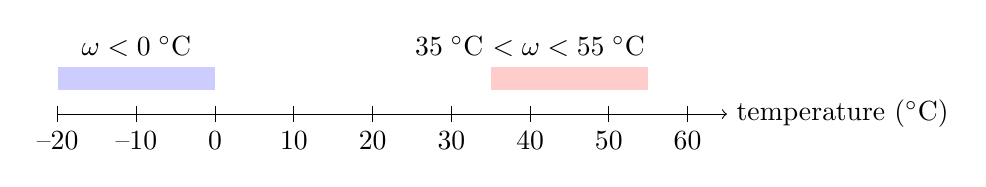
\begin{tikzpicture}
			% Draw temperature axis
			\draw[->] (0,0) -- (8.5,0) node[right] {temperature ($^\circ$C)};
			% Add tick marks and labels every 20 degrees from -20 to 100
			\foreach \x/\label in {0/--20, 1/--10, 2/0, 3/10, 4/20, 5/30, 6/40, 7/50, 8/60} {
			\draw (\x,0.1) -- (\x,-0.1);
			\node[below] at (\x,-0.1) {\label};
			}
			% Shade measurable set: Temperature < 0°C
			\fill[blue!20] (0,0.3) rectangle (2,0.6);
			\node[above] at (1,0.6) {$\omega< 0\;^\circ$C};
			% Shade measurable set: 5°C < omega < 10°C
			\fill[red!20] (5.5,0.3) rectangle (7.5,0.6);
			\node[above] at (6,0.6) {$35\;^\circ$C $< \omega< 55\;^\circ$C};
			\vspace*{10mm}
			\end{tikzpicture}
			\vspace*{10mm}
			\end{center}
			\caption{A sample space constituted by all possible temperature values $\omega$ 
			that can occur at an Finnish Meteorological Institute (FMI) station. Two measurable subsets of temperature 
			values, denoted by $\mathcal{A}^{(1)}$ and $\mathcal{A}^{(2)}$, are highlighted. For any 
			actual temperature value $\omega$, it is possible to determine (via some equipment) 
			whether $\omega\in \mathcal{A}^{(1)}$ and whether $\omega\in \mathcal{A}^{(2)}$. 
			\label{fig_measurable_dict}} 
		\end{figure}
		In principle, measurable sets could be chosen freely (e.g., depending on the resolution of the 
		measuring equipment). However, it is often useful to impose certain completeness requirements 
		on the collection of measurable sets. For example, the sample space itself should be 
		measurable, and the union of two measurable sets should also be measurable. These completeness 
		requirements can be formalized via the concept of a $\sigma$-algebra (or $\sigma$-field) 
		\cite{RudinBook}, \cite{BillingsleyProbMeasure}, \cite{durrett2010probability}. 
		A measurable space is a pair $\big(\mathcal{X},\mathcal{F}\big)$ that consists of an arbitrary 
		set $\mathcal{X}$ and a collection $\mathcal{F}$ of measurable subsets of $\mathcal{X}$ 
		that form a $\sigma$-algebra. 
		\\
		See also: sample space, outcome, $\sigma$-algebra, probability.},
	first={measurable},
	type=math, 
	text={measurable} 
}

\newglossaryentry{sigmaalgebra}
{name={$\sigma$-algebra}, 
sort={sigma-algebra},
	description={Consider a random experiment with a sample space $\Omega$. 
		A $\sigma$-algebra\index{$\sigma$-algebra} (or $\sigma$-field) $\Sigma$ 
		is a collection of subsets of $\Omega$ with the following properties 
		\cite{RudinBook}, \cite{BillingsleyProbMeasure}, \cite{durrett2010probability}:
		\begin{itemize}
		 	\item The empty set $\emptyset$ and the entire sample space 
		 	$\Omega$ belong to $\Sigma$, i.e., $\emptyset \in \Sigma$ and $\Omega\in \Sigma$.
		 	\item If a set $\mathcal{A}$ belongs to $\Sigma$, then its complement 
		 	$\Omega\setminus \mathcal{A}$ also belongs to $\Sigma$, i.e., 
		 	$\mathcal{A} \in \Sigma$ implies $\Omega\setminus \mathcal{A} \in \Sigma$.
		 	\item If a countable collection of sets $\mathcal{A}_1, \,\mathcal{A}_2, \,\ldots$ belongs 
			to $\Sigma$, 
		 	then their union also belongs to $\Sigma$, i.e.,
		 	$\mathcal{A}_1, \,\mathcal{A}_2, \,\ldots \in \Sigma$ implies 
		 	$\bigcup_{i=1}^{\infty} \mathcal{A}_i \in \Sigma$.	
		 \end{itemize}			 
		See also: sample space, random variable (RV), probability space.},
	first={$\sigma$-algebra},
	type=math, 
	text={$\sigma$-algebra} 
}

\newglossaryentry{sigmafield}
{name={$\sigma$-field}, 
sort={sigma-field},
	description={See $\sigma$-algebra\index{$\sigma$-field}.}, 
	first={$\sigma$-field},
	type=math,
	text={$\sigma$-field} 
}

\newglossaryentry{injective}
{name={injective}, 
	description={A function $f: \mathcal{U} \rightarrow \mathcal{V}$ is injective\index{injective} 
		if it maps distinct elements of its domain to distinct elements 
		of its co-domain, 
    		i.e., if $f(u_1) = f(u_2)$ implies $u_1 = u_2$ for all $u_1, u_2 \in \mathcal{U}$ 
        		\cite{HalmosSet}. 
    		Equivalently, no two different function inputs are mapped to the same function output.
				\\
		See also: function.},
	first={injective},
	type=math,
	text={injective} 
}

\newglossaryentry{typicalset}
{name={typical set}, 
	description={See probability mass function (pmf)\index{typical set}.}, 
 	first={typical set},
 	firstplural={typical sets},
 	type=math,
 	plural={typical sets},
 	text={typical set} 
}

\newglossaryentry{majmin}
{name={majorize-minimize (MM)}, 
	description={Consider an optimization problem $\min_{{\bf w}\in \mathcal{W}} f({\bf w})$ with 
		some complicated (potentially non-convex and non-smooth) objective function. 
		One important example of such an optimization problem is empirical risk minimization (ERM), which is used to learn the 
		model parameters of a nonlinear model. 
		An MM method is\index{majorize-minimize (MM)} an iterative optimization method 
		that constructs a sequence ${\bf w}^{(1)},\,{\bf w}^{(2)},\,\ldots \in \mathcal{W}$ 
		of model parameters as follows \cite{Lange2016MM}, \cite{BishopBook}, \cite{Hunter01022004}
		(see also Fig. \ref{fig:majmin_dict}): 
		\begin{itemize} 
			\item During the $t$th iteration, the objective function $f(\cdot)$ 
			 	is approximated by another function $g\big(\cdot;{\bf w}^{(t)}\big)$.
	             	  	This approximation must be an upper bound for (i.e., must majorize) the original
				objective function, i.e., $g\big({\bf w};{\bf w}^{(t)}\big) \geq f({\bf w})$ 
			 	for all ${\bf w}\in \mathcal{W}$, and it must be tight for ${\bf w}^{(t)}$, i.e., 
			 	$g\big({\bf w}^{(t)};{\bf w}^{(t)}\big) = f\big({\bf w}^{(t)}\big)$.
			\item The new model parameters  ${\bf w}^{(t+1)}$ are then obtained by 
				minimizing the approximation, i.e., 
				 ${\bf w}^{(t+1)} \in \argmin_{{\bf w}\in \mathcal{W}}g\big({\bf w};{\bf w}^{(t)}\big)$. 
		\end{itemize} 
		\begin{figure}[H]
			 \centering
			 \begin{tikzpicture}[x=1.2cm,y=1cm]
				% --- parameters ---
				\def\xa{0}
				\def\xb{2*pi}
				\def\xo{3*pi/4}     % touch point: 1.5 * (pi/2) = 3pi/4
				\def{\bf L}{0.4}        % left slope  (adjust to keep it above the sine)
				\def{\bf R}{0.7}        % right slope (adjust to keep it above the sine)
				% horizontal axis
				\draw[->] (\xa-0.2,-2) -- (\xb+0.3,-2) node[right] {${\bf w}$};
				% sine over one period
				\draw[thick,samples=100,domain=\xa:\xb]
				plot (\x,{sin(\x r)}) node[pos=0.1,above left,black] {\small $f({\bf w})$};
				% compute y0 = sin(w0)
				\pgfmathsetmacro\yxo{sin(\xo r)}
				% Anchors (numeric, no macros)
				% w0 = 3*pi/4 = 2.35619449
				% xL = 2.00619449, xR = 2.70619449
				% y0 = sin(w0) = 0.70710678
				% Left slope mL = cos(xL) = -0.42177145  (tangent => upper bound on [0, xL])
				% Right slope mR = 0.7  (rising; safely above the sine on [xR, 2*pi])
				\def\xL{2.70}
				\def\xR{3.80}
				\def\yO{0.70}
				% Left (tangent) segment: y = y0 + mL*(x - xL), mL = -0.42177145
				\draw[dashed,samples=2,domain=0:\xL]
				plot (\x,{\yO + (-0.7)*(\x - \xo)});
				% Flat touching segment
				\draw[dashed]
				(\xL,{\yO+(-0.7)*(\xL-\xo)}) -- (\xR,{\yO+(-0.7)*(\xL-\xo)});
				% Right rising segment: y = y0 + mR*(x - xR), mR = 0.7
				% draw the segment
				\draw[dashed,samples=2,domain=\xR:2*pi]
				plot (\x,{\yO+(-0.7)*(\xL-\xo) + (0.7)*(\x - \xR)});
				% compute a point 65% along the x-range [\xR, 2*pi]
				\pgfmathparse{\xR + 0.65*(2*pi - \xR)} \let\xmid\pgfmathresult
				\pgfmathparse{\yO + 0.7*(\xmid - \xR)} \let\ymid\pgfmathresult
				% label at that point
				\node[right,black] at (\xmid,\ymid) {$g\big( {\bf w}; {\bf w}^{(t)} \big)$};
				% Touch marker at w0
				\fill[red] (2.35619449,0.70710678) circle (1.2pt);
				% --- vertical ruler marking w0 ---
				\draw[densely dotted,gray] (\xo,-2) -- (\xo,\yO);
				% \draw[gray] (\xo,0) -- ++(0,-2.06);
				\node[below] at (\xo,-2) {${\bf w}^{(t)}$};
			\end{tikzpicture}
		\caption{The construction of model parameters based on the iterative MM method.}
			\label{fig:majmin_dict}
		\end{figure}
		Similar to gradient-based methods, the MM principle is also based on approximating an 
		objective function locally, around the current model parameters, and then optimizing 
		this approximation to obtain new model parameters. However, the construction 
		of local approximations is very different. While gradient-based methods use linear functions 
		for these approximations, MM methods can use nonlinear functions as long as 
		they are upper bounds for the original objective function. 
			 \\ 
		See also: gradient-based method, expectation–maximization (EM).},
	first={majorize–minimize (MM)},
	type=math, 
	text={MM}
}

\newglossaryentry{markovsinequality}
{name={Markov's inequality},
	description={Consider a real-valued nonnegative random variable (RV) $x$ for which 
		the expectation $\mathbb{E} \{ x\}$ exists. \index{Markov's inequality} 
	 	Markov's inequality provides an upper bound on the probability 
	 	$\mathbb{P}\left(x\geq a\right)$ that $x$ exceeds a given positive threshold $a>0$.  
	 	In particular,          
	 	\begin{equation}
            		\nonumber
			\mathbb{P}\left(x \geq a\right) \leq \frac{\mathbb{E} \{ x\}}{a} \qquad \mbox{ holds for any } a > 0. 
            		%\label{eq:markovsinequality_dict}
    		\end{equation}
    		This inequality can be verified by noting that $\mathbb{P}\left(x \geq a\right)$ is the 
		expectation $\mathbb{E} \{g(x)\}$ with the function 
	 	$$g: \mathbb{R} \rightarrow \mathbb{R}: x' \mapsto \mathbb{I}_{\{x \geq a\}}(x').$$ 
	 	As illustrated in Fig. \ref{fig:markovsinequality_dict}, for any positive $a>0$, 
	 	$$ g(x') \leq x'/a \mbox{ for all } x' \in \mathbb{R}.$$ 
	 	This implies Markov's inequality via the monotonicity property 
	 	of the Lebesgue integral \cite[p. 50]{folland1999real}. 
    		\begin{figure}[H]
			\centering
			\begin{tikzpicture}[scale=1, x=0.8cm, y=0.8cm]
			% -------- parameters ----------
			\def\a{3.24}      % threshold a
			\def\xmax{10}     % x-axis max
			\def\m{0.02}      % slope of the linear function y = m(x-a)+1
			% -------- pdf function p(x) (same as your expression) ----------
			% p(x) = (1/(3*sqrt(2*pi))) * x^(1.5) * exp(-x/2)
			\draw[-{Latex}] (0,0) -- (\xmax+1,0) node[below right] {$x'$};
			%\draw[-{Latex}] (0,0) -- (0,3.1) node[left] {$\pdf{x}{x'}$};
                		\draw[-{Latex}] (0,0) -- (0,3.1)  node[left, text=blue!70!black] {$p^{(x)}\left(x'\right)$};
			% Fill under the pdf (optional aesthetics)
			\fill[blue!15, opacity=0.3]
			plot[samples=400, domain=0:\xmax, smooth]
			(\x,{ (6/sqrt(2*pi)) * (\x)^(1.5) * exp(-\x/2) }) -- (\xmax,0) -- (0,0) -- cycle;
			% PDF curve
			\draw[blue!70!black, very thick, samples=400, domain=0:\xmax, smooth]
			plot (\x,{ (6/(sqrt(2*pi))) * (\x)^(1.5) * exp(-\x/2) })
			node[pos=0.9, above right, xshift=2pt] {};
			% Vertical guide at x=a
			\draw[dashed, gray] (\a,0) -- (\a,1.05);
			\node[below] at (\a,0) {$a$};
			\node[above] at (1*\a,3) {$\mathbb{P}\left(x \geq a\right) \leq \frac{\mathbb{E} \{ x\}}{a}$}; 
			\node[below] at (0,0) {$0$};
			% -------- indicator 1{x >= a} ----------
			% 0 for x<a with open circle at (a,0)
			\draw[green!60!black, ultra thick] (0,0) -- (\a,0);
			\filldraw[white, draw=green!60!black, line width=0.8pt] (\a,0) circle (2pt);
			% 1 for x>=a with closed circle at (a,1)
			\draw[green!60!black, ultra thick] (\a,1) -- (\xmax,1)
			node[pos=0.9, above, yshift=2pt] {$\mathbb{I}_{\{x \ge a\}}(x')$};
			\filldraw[green!60!black] (\a,1) circle (2pt);
			% -------- linear curve through (a,1): y = m(x-a)+1 ----------
			\draw[red!70, very thick, samples=2, domain=0:\xmax]
			plot (\x,{ \x*(1/\a) }); 
			\node[align=right,red!70,yshift=20pt] at ({2.5*\a+0.2},{2.5}) {$f(x') = x'/a$};  
			% Axis marker for y=1
			\draw (0,1) -- ++(-0.12,0) node[left] {$1$};
			\end{tikzpicture}
            	\caption{The expectation $\mathbb{E} \{x\}$ and the probability $\mathbb{P}\left(x \geq a\right)$ 
			of a nonnegative random variable (RV) $x$ with a probability density function (pdf) $p^{(x)}\left(\cdot\right)$           
                		%a \gls{probdist} $\probdist^{(x)}$ 
			can be obtained via Lebesgue integrals of 
			$f(x') = x'/a$ and $g(x') = \mathbb{I}_{\{x \geq a\}}(x')$, respectively.}
            		\label{fig:markovsinequality_dict}
        		\end{figure} 
		See also: expectation, probability, concentration inequality.},
	first={Markov's inequality},
	type=math, 
    	text={Markov's inequality}  
}

\newglossaryentry{chebyshevsinequality}
{name={Chebyshev's inequality},
	description={Consider a real-valued random variable (RV) $x$ for which 
		the second moment $\mathbb{E} \{ x^{2} \}$ exists (and is finite). 
 	 	The existence of the second moment implies the existence 
 	 	of a finite expectation $\mu :=\mathbb{E} \{ x\}$ and a finite 
 	 	variance $\sigma^{2}\!:=\!\mathbb{E} \big\{ \big( x\!-\!\mu \big)^{2} \big\}$ \cite[Proposition 6.12]{folland1999real}. 
 	 	Chebyshev's inequality\index{Chebyshev's inequality} refers 
 	 	to the following upper bound on the probability that $x$ 
 	 	deviates from $\mu$ by more than a given threshold $\eta$ 
 	 	\cite[Ch. 4]{FellerBook}. 
 	 	In particular,   
 		\begin{equation}
           		\nonumber
			\mathbb{P}\left(\big|x - \mu \big| \geq \eta \right) \leq \frac{\sigma^2}{\eta^2} \qquad \mbox{ for any } \eta > 0.
            		%\label{eq:chebyshevsinequality_dict}
     		\end{equation}
 		This upper bound can be obtained by applying Markov's inequality to 
 		the new random variable (RV) $\tilde{x}\!:=\! \big(x\!-\!\mu \big)^2$. 
  		\begin{figure}[H]
   			\centering
			\begin{tikzpicture}
     			\begin{axis}[
      			width=9cm, height=4.2cm,
      			samples=300,
      			axis lines=left,
	  		ylabel={$p^{(x)}\left(x'\right)$},
      			xlabel={$x'$},
      			x label style={at={(axis description cs:1,0)}, anchor=west},
	  		ylabel style={rotate=270,anchor=south,at={(axis description cs:0,1.02)}},
      			xtick={-1.5,0,1.5},
      			xticklabels={$-\eta$,$\mu$,$\eta$},
      			ytick=\empty,
      			ymin=0, ymax=0.45,
      			domain=-4:4,
      			clip=false
    			]
      			% pdf (centered at mu; here shown as standard normal in x - mu coordinates)
      			\addplot[name path=pdf, black, very thick] {exp(-0.5*x^2)/sqrt(2*pi)};
      			\addplot[name path=axis, draw=none] {0};
      			% shaded tails: |X - mu| >= t with t = 1.5
      			\addplot[red!70, opacity=0.25] fill between[of=pdf and axis, soft clip={domain=1.5:4}];
      			\addplot[red!70, opacity=0.25] fill between[of=pdf and axis, soft clip={domain=-4:-1.5}];
      			% guide lines at mu and ±t
      			\draw[densely dashed] (axis cs:0,0) -- (axis cs:0,0.42);
      			\draw[dashed] (axis cs:1.5,0) -- (axis cs:1.5,{exp(-0.5*1.5^2)/sqrt(2*pi)});
      			\draw[dashed] (axis cs:-1.5,0) -- (axis cs:-1.5,{exp(-0.5*1.5^2)/sqrt(2*pi)});
      			% label for the shaded area
   			%   \node[anchor=west] at (axis description cs:0.72,0.82) {$\prob{|x-\mu|\ge \eta}$};
    			\end{axis}
  			\end{tikzpicture}
  		\caption{Chebyshev's inquality provides an upper bound on 
              		the tail probability $\mathbb{P}\left(|x-\mu|\ge \eta\right)$ (i.e., shaded area) of
			a real-valued random variable (RV) $x$ with a finite second moment.\label{fig:chebyshev_minimal_dict}} 
		\end{figure}
     		See also: expectation, Markov's inequality, concentration inequality.},
    	first={Chebyshev's inequality},
	type=math, 
     	text={Chebyshev's inequality}  
}

\newglossaryentry{hoeffdingsinequality}
{name={Hoeffding's inequality},
	description={\index{Hoeffding's inequality} Hoeffding's inequality \cite{Hoeffding1963} is a fundamental concentration inequality 
		that provides an upper bound on the probability that a sum (or average) of independent, bounded random variables (RVs) 
		deviates from its mean by more than some threshold. 
     		Let $x_1,\,\dots,\,x_n$ be independent real-valued random variables (RVs) $x_i$ taking values in $[a_i,b_i] \subset \mathbb{R}$, 
		and $S_n :=\sum_{i=1}^n x_i$ and $\mathbb{E} \{S_n\} = \sum_{i=1}^n \mathbb{E} \{x_i\}$. 
		Then, Hoeffding's inequality \cite[Th. 2.2.6]{vershynin2018high} states that
        		\begin{equation}
                		\nonumber
			\mathbb{P}\left( |S_n - \mathbb{E} \{S_n\}| \geq t \right) 
            		\leq 2 \exp \left( -\frac{2 t^2}{\sum\limits_{i=1}^n (b_i - a_i)^2} \right) \qquad \forall t > 0.
            		%\label{eq:hoeffding_sum}
        		\end{equation}
    		Hoeffding's inequality typically provides sharper bounds than Chebyshev's inequality, 
		but it is more restrictive by assuming bounded random variables (RVs).
    		In the context of machine learning (ML), this result is useful for deriving guarantees for empirical risk minimization (ERM)  and in the context of MAB. 
		 \\
    		See also: concentration inequality, probability, random variable (RV), Chebyshev's inequality, expectation, probability space, Markov's inequality.},
    	first={Hoeffding's inequality},
	type=math, 
    	text={Hoeffding's inequality}  
}

\newglossaryentry{rgg}
{name={random geometric graph (RGG)},
	description={An RGG\index{random geometric graph (RGG)} is a probabilistic model for graphs 
		built from nodes randomly placed in a metric space. Given a metric space, the RGG is characterized by 
		the number of nodes, the connection radius, and the probability distribution describing the node placement. 
    		More precisely, for a node set $i=1, \,\ldots, \,n$, each node $i$ is assigned to a random position 
		${\bf x}^{(i)} \in \mathcal{X}$, typically as realizations of independent and identically distributed (i.i.d.) random variables (RVs) taking values in a set $\mathcal{X}$. 
		Together with a metric, this forms a metric space, often with the metric induced by a norm. 
		A specific realization of an RGG contains an edge $\{i,i'\}$ if and only if the distance between the nodes 
		with respect to the metric is smaller than some threshold, i.e., when $d({\bf x}^{(i)},{\bf x}^{(i')})\leq r$ 
		for some threshold $r>0$, as illustrated in Fig. \ref{fig:rgg}.
         	\begin{figure}[H]
    			\centering
    			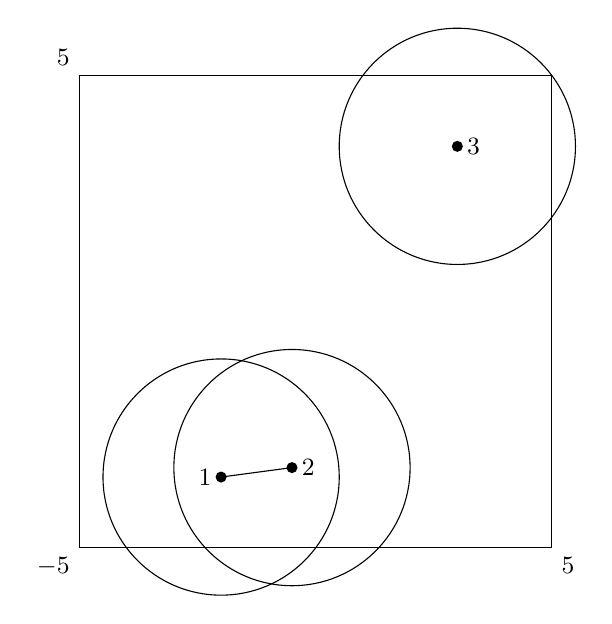
\begin{tikzpicture}[x=0.6cm,y=0.6cm]
        				\draw (-5,-5) rectangle (5,5);
        				% Corner labels outside the rectangle
        				\node[below left] at (-5,-5) {\small $-5$};
        				\node[above left]  at (-5, 5) {\small $5$};
        				\node[below right] at ( 5,-5) {\small $5$};
        				% Bottom two points (nodes 1 and 2) within each other's circle of radius 2.5
        				\fill (-2.0,-3.5) circle (2pt);
        				\draw (-2.0,-3.5) circle (2.5);
        				\node[anchor=east] at (-2.0,-3.5) {\small 1};
        				\fill (-0.5,-3.3) circle (2pt);
        				\draw (-0.5,-3.3) circle (2.5);
        				\node[anchor=west] at (-0.5,-3.3) {\small 2};
        				\draw (-2.0,-3.5) -- (-0.5,-3.3);
        				% Top point (node 3) outside the bottom circles
        				\fill (3.0,3.5) circle (2pt);
        				\draw (3.0,3.5) circle (2.5);
        				\node[anchor=west] at (3.0,3.5) {\small 3};
    			\end{tikzpicture}
   		\caption{Illustration of an RGG with $ \mathcal{X}= [-5,5]\times[-5,5] \subset \mathbb{R}^2$ and radius $r=2.5$ 
			(with respect to the Euclidean distance), where nodes 1 and 2 (corresponding to $(-2.0, -3.5)^T$ and $(-0.5, -3.3)^T$, 
			within radius $r=2.5$) are connected, while node 3 (corresponding to $(3.0, 3.5)^T$) has no other node within that distance.}
    			\label{fig:rgg}
    		\end{figure}
        		See also: graph, stochastic block model (SBM), Erd\H{o}s–R\'enyi graph (ER graph).},
    	first={random geometric graph (RGG)},
	type=math, 
    	text={RGG}
}

\newglossaryentry{banachfixedpoint}
{name={Banach's fixed-point theorem},
	description={Banach's fixed-point theorem\index{Banach's fixed-point 
		theorem} (also referred to as the contraction principle \cite[Th. 9.23]{RudinBookPrinciplesMatheAnalysis},\cite{Kelley1995}) 
		states that every contractive operator $\mathcal{F}$ on a complete 
		metric space $\mathcal{W}$ has a unique fixed point. 
		Formally, let $(\mathcal{W},d(\cdot,\cdot))$ be a non-empty 
		complete metric space and let $\mathcal{F}:\mathcal{W}\to\mathcal{W}$ satisfy
    		\[
    		d(\mathcal{F}{\bf w},\mathcal{F}{\bf w}') \leq \kappa\cdot d({\bf w},{\bf w}') \qquad \forall {\bf w},{\bf w}'\in\mathcal{W}\]
    		for some constant $\kappa\in [0,1)$. Then, $\mathcal{F}$ has a unique fixed point, 
		i.e., there exists a unique ${\bf w}^\star\in\mathcal{W}$ with 
		$\mathcal{F}{\bf w}^\star ={\bf w}^\star$. Moreover, for any initial 
		${\bf w}^{(0)}\in\mathcal{W}$, the fixed-point iteration 
		${\bf w}^{(t)}\!=\!\mathcal{F}{\bf w}^{(t-1)}$, for $t=1,\,2,\,\dots$, 
		converges to ${\bf w}^\star$ at a rate governed by $\kappa$. 
		In particular, 
		\[ d({\bf w}^{(t)},{\bf w}^\star) \leq \kappa^{t}
		 \cdot d({\bf w}^{(0)},{\bf w}^\star) \mbox{, for }t=1,\,2,\,\dots. \]   		
		\begin{figure}[H]
    			\centering
    			\begin{tikzpicture}[>=Latex, font=\small]
    			\tikzset{space/.style={draw, thick, circle, minimum size=4.0cm},pt/.style={circle, inner sep=1.5pt, draw, fill=black},maparrow/.style={->, very thick},link/.style={->, thick},distline/.style={dashed, thick}}
    			\def\dx{6.5}
    			\node[space,label=above:{$\mathcal{W}$}] (XL) at (0,0) {};
    			\node[space,label=above:{$\mathcal{W}$}] (XR) at (\dx,0) {};
    			\draw[maparrow] (XL.east) -- node[above=2pt] {$\mathcal{F}$} (XR.west);
    			\coordinate (x1) at (-0.8,0.9);
    			\coordinate (x2) at (0.9,0.5);
    			\node[pt,label=above left:{${\bf w}$}] at (x1) {};
    			\node[pt,label=right:{${\bf w}'$}] at (x2) {};
    			\coordinate (fx1) at (\dx-0.3,0.5);
    			\coordinate (fx2) at (\dx+0.6,0.5);
    			\node[pt] (FX1) at (fx1) {};
    			\node[pt] (FX2) at (fx2) {};
    			\node[anchor=east] at ($(FX1.west)+(-6pt,-2pt)$) {$\mathcal{F}{\bf w}$};
    			\node[anchor=west] at ($(FX2.east)+(6pt,-2pt)$) {$\mathcal{F}{\bf w}'$};
   			% \draw[distline] (x1) -- (x2) node[midway, above=6pt, sloped] {$\metric{\fixedpointop \weights}{\fixedpointop \weights'}$};
   			% \draw[distline] (fx1) -- (fx2) node[midway, above=6pt, sloped] {$\metric{\weights}{\weights'}$};
    			\coordinate (xsL) at (0,-0.9);
    			\coordinate (xsR) at (\dx,-0.9);
    			\node[pt,label=below:{${\bf w}^\star$}] at (xsL) {};
    			\node[pt,label=below:{$\mathcal{F}{\bf w}^\star\!=\!{\bf w}^\star$}] at (xsR) {};
    			\end{tikzpicture}
   	 	\caption{A contractive operator $\mathcal{F}:\mathcal{W}\to\mathcal{W}$  
	  		has a unique fixed point ${\bf w}^\star$ with 
			$\mathcal{F}{\bf w}^\star\!=\!{\bf w}^\star$.}
    			\label{fig:banach_dict}
    		\end{figure}
    		See also: contractive operator, fixed-point iteration.},
    	first={Banach's fixed-point theorem},
	text={Banach's fixed-point theorem},
    	type=math
}

\newglossaryentry{cvxoptproblem}
{name={convex optimization problem}, 
	description={See\index{convex optimization problem} convex optimization.},
	first={convex optimization problem},
	firstplural={convex optimization problems}, 
	type=math,
	plural={convex optimization problems}, 
	text={convex optimization problem}
}

\newglossaryentry{optimization}
{name={optimization}, 
	description={See\index{optimization} convex optimization, optimization method, optimization problem.},
	first={optimization},
	firstplural={optimizations}, 
	type=math,
	plural={optimizations}, 
	text={optimization}
}

\newglossaryentry{optproblem}
{name={optimization problem}, 
	description={An\index{optimization problem} optimization problem is a mathematical 
		   structure consisting of an objective function $f: \mathcal{U} \rightarrow \mathcal{V}$ 
		   defined over an optimization variable ${\bf w}\in \mathcal{U}$, together with a 
		   feasible set $\mathcal{W}\subseteq \mathcal{U}$. The co-domain $\mathcal{V}$ is 
		   assumed to be ordered, meaning that for any two elements $\mathbf{a}, \mathbf{b} \in \mathcal{V}$, 
		   we can determine whether $\mathbf{a} \leq \mathbf{b}$.
		   Here, ``$\leq$'' denotes a general partial order relation, which may differ from the standard 
		   numerical order on real numbers \cite[Sec. 2.4]{BoydConvexBook}. 
		   The goal in optimization is to find those values ${\bf w}\in \mathcal{W}$ 
		   for which the objective $f({\bf w})$ is extremal—i.e., minimal or maximal 
		   \cite{BoydConvexBook}, \cite{BertsekasNonLinProgr}, \cite{nesterov04}.
		   \\
		   See also: objective function.},
	first={optimization problem},
	firstplural={optimization problems}, 
	type=math,
	plural={optimization problems}, 
	text={optimization problem}
}

\newglossaryentry{optmethod}
{name={optimization method},
	description={An\index{optimization method} optimization method is 
		an algorithm that takes a representation of an 
		optimization problem as input and computes an (approximate) 
		solution as its output. A central example of an optimization problem 
		in machine learning (ML) is empirical risk minimization (ERM). By applying an appropriate 
		optimization method to empirical risk minimization (ERM), we obtain a concrete learning 
		algorithm \cite{BoydConvexBook}, \cite{BertsekasNonLinProgr},
		\cite{nesterov04}.
		 \\
		 See also: algorithm, optimization problem.},
	type=math, 
	first={optimization method},
	firstplural={optimization methods}, 
	plural={optimization methods}, 
	text={optimization method}
}

\newglossaryentry{convexopt}
{name={convex optimization},
 	description={Convex optimization\index{convex optimization} studies the 
		formulation, properties, and efficient solution methods for convex optimization problems \cite{BoydConvexBook}.  
		A convex optimization problem (defined on the Euclidean space $\mathbb{R}^{d}$) 
		consists of a convex objective function $f: \mathbb{R}^{d} \rightarrow \mathbb{R}$  
    		and a convex constraint set $\mathcal{C}$ for the optimization variable ${\bf w}$.  
    		It can be written compactly as \cite{BoydConvexBook}
		$$ \min_{{\bf w}\in \mathcal{C}}  f({\bf w}).$$ 
		Alternatively, a convex optimization problem can be expressed in 
		terms of convex constraint functions $g_1,\,\ldots,\,g_k$ as
		\begin{align} 
			\min_{{\bf w}\in \mathbb{R}^{d}} & f({\bf w})   \nonumber \\ 
			\mbox{s.t.} \quad & g_{r}({\bf w}) \leq 0, \quad r=1,\,\ldots,\,k. \label{equ_def_convx_opt_constr_dict}
		\end{align} 
		\begin{figure}[H]
			\centering
			\begin{tikzpicture}[>=stealth, scale=1.0]
  			% Axes
  			\draw[->] (-3,0) -- (5.2,0) node[below] {${\bf c}$};
  			\draw[->] (0,-0.2) -- (0,4.2) node[left] {$t$};
  			% Exponential boundary: t = 3 e^{-g}
  			\draw[thick, domain=-1:3, smooth, variable=\x, name path=boundary]
    			plot ({\x},{exp(-\x)});%node[pos=0.45, below right] {};
  			% Transparent epigraph region (above the curve)
  			\path[fill=gray!40, opacity=0.4]
    			(-1,3) -- (-1,{exp(1)}) -- plot[domain=-1:3] ({\x},{exp(-\x)})
   			-- (3,3) -- cycle;
  			% Crossing with vertical axis (g=0): mark and label f^*
  			\fill (0,1) circle (1.6pt) node[left] {$f^{\ast}$};
  			% Tangent at g=1: slope = -e^{-1}, passes through (1, e^{-1})
  			% Equation: t = (2/e) - (1/e) * g
  			\draw[dashed, domain=-1:3, smooth, variable=\x]
    			plot ({\x},{(2/exp(1)) - (1/exp(1))*\x}); 
   			% node[pos=0.15, above right] {tangent at $g=1$};
  			% (Optional) mark the point of tangency
  			\fill (1,{1/exp(1)}) circle (1.2pt);
  			% Label for shaded region
  			\node at (2.6,2.5) {$\mathcal{A}$};
  			\node [below,yshift=-3pt] at (0,-0.2) {$\mathbf{0}$};
  			\end{tikzpicture}
  		\caption{A convex optimization problem \eqref{equ_def_convx_opt_constr_dict} can be represented 
  			by a set $\mathcal{A}$ that consists of objective values $t$ and constraint values 
  			${\bf c}=\big(c_{1},\,\ldots,\,c_{d}\big)^{T}$ that are achievable, i.e., 
  			$f({\bf w}) \leq t, g_{1}({\bf w})\leq c_{1},\,\ldots, \,g_{k}({\bf w}) \leq c_{k}$ 
  			for some ${\bf w}\in \mathbb{R}^{d}$. The optimal value $f^{\ast}$ of the 
  			optimization problem is the smallest $t$ for which $(\mathbf{0},t) \in \mathcal{A}$. }
		\end{figure}
		The formulation \eqref{equ_def_convx_opt_constr_dict} lends, in turn, to the 
		epigraph form of \cite[Sec. 5.3]{BoydConvexBook} 
		$$\inf \big\{ t \in \mathbb{R} : (\mathbf{0}, t) \in \mathcal{A} \big\}$$ 
		with the set 
		\begin{align} 
			\mathcal{A} :=\big\{ ({\bf c},t) & \in \mathbb{R}^{d} \times \mathbb{R} : 
    			f({\bf w}) \leq t, \, \nonumber \\ 
   			&  g_{r}({\bf w}) \leq c_{r}, \,
    			r= 1,\,\ldots,\,k, 
    			\text{ for some } {\bf w}\in \mathbb{R}^{d} \big\}. \nonumber
		\end{align}
		It can be shown that, since $f,g_{1},\,\ldots,\,g_{k}$ are convex functions, 
    		$\mathcal{A}$ is a convex set \cite[Ch. 2]{BoydConvexBook}.
		The set $\mathcal{A}$ fully characterizes the optimization problem~\eqref{equ_def_convx_opt_constr_dict} 
		and can be interpreted as the epigraph of the objective function~$f$ over the 
		feasible region defined by the constraint functions $g_1,\,\ldots,\,g_k$.
		\\ 
    		See also: convex, optimization problem, optimization method. },
	first={convex optimization},
	type=math,
  	text={convex optimization}
}

\newglossaryentry{newtonmethod}
{name={Newton's method},
	description={Newton's method\index{Newton's method} is an iterative optimization method for finding 
		local minima or maxima of a differentiable objective function $f({\bf w})$. 
		Like gradient-based methods, Newton's method also 
		computes a new estimate $\widehat{{\bf w}}_{t+1}$ by optimizing a local approximation of $f({\bf w})$ around 
		the current estimate $\widehat{{\bf w}}_{t}$. In contrast to gradient-based methods, which use the gradient to build 
		a local linear approximation, Newton's method uses the Hessian matrix to build a local quadratic approximation. 
		In particular, starting from an initial estimate $\widehat{{\bf w}}_{0}$, Newton's method iteratively updates the estimate according to 
		\[
		\widehat{{\bf w}}_{t+1}= \widehat{{\bf w}}_{t}- \big( \nabla^2 f\big(\widehat{{\bf w}}_{t}\big) \big)^{-1} \nabla f\big( \widehat{{\bf w}}_{t} \big) \mbox{, for } t=0,\,1,\,\ldots.
		\]
		Here, $\nabla f\big(\widehat{{\bf w}}_{t} \big)$ is the gradient, and $\nabla^2 f({\bf w}^{(t)})$ is 
		the Hessian of the objective function $f$. Since using a quadratic function as local approximation is more accurate 
		than using a linear function (which is a special case of a quadratic function), Newton's method tends to 
		converge faster than gradient-based methods (see Fig. \ref{fig_newtonmethod_dict}). However, this faster convergence comes at the increased computational 
		complexity of the iterations. Indeed, each iteration of Newton's method requires the inversion of the Hessian. 
		\begin{figure}[H]
		\centering
		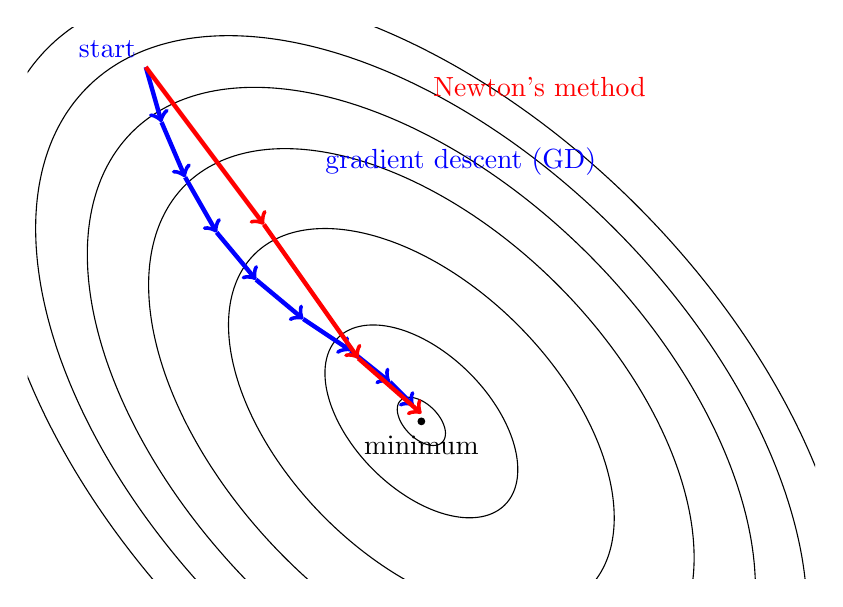
\begin{tikzpicture}[samples=200,smooth]
			\begin{scope}
				\clip(-5,-2) rectangle (5,5);
				\draw[thin] plot[domain=0:360] ({1.5*cos(\x)*sqrt(20/(sin(2*\x)+2))},{1.5*sin(\x)*sqrt(20/(sin(2*\x)+2))});
				\draw[thin] plot[domain=0:360] ({1.5*cos(\x)*sqrt(16/(sin(2*\x)+2))},{1.5*sin(\x)*sqrt(16/(sin(2*\x)+2))});
				\draw[thin] plot[domain=0:360] ({1.5*cos(\x)*sqrt(12/(sin(2*\x)+2))},{1.5*sin(\x)*sqrt(12/(sin(2*\x)+2))});
				\draw[thin] plot[domain=0:360] ({1.5*cos(\x)*sqrt(8/(sin(2*\x)+2))},{1.5*sin(\x)*sqrt(8/(sin(2*\x)+2))});
				\draw[thin] plot[domain=0:360] ({1.5*cos(\x)*sqrt(4/(sin(2*\x)+2))},{1.5*sin(\x)*sqrt(4/(sin(2*\x)+2))});
				\draw[thin] plot[domain=0:360] ({1.5*cos(\x)*sqrt(1/(sin(2*\x)+2))},{1.5*sin(\x)*sqrt(1/(sin(2*\x)+2))});
				\draw[thin] plot[domain=0:360] ({1.5*cos(\x)*sqrt(0.0625/(sin(2*\x)+2))},{1.5*sin(\x)*sqrt(0.0625/(sin(2*\x)+2))});
				% Gradient Descent path
				\draw[->,blue,ultra thick] (-3.5,4.5) -- (-3.3,3.8);
				\draw[->,blue,ultra thick] (-3.3,3.8) -- (-3,3.1);
				\draw[->,blue,ultra thick] (-3,3.1) -- (-2.6,2.4);
				\draw[->,blue,ultra thick] (-2.6,2.4) -- (-2.1,1.8);
				\draw[->,blue,ultra thick] (-2.1,1.8) -- (-1.5,1.3);
				\draw[->,blue,ultra thick] (-1.5,1.3) -- (-0.9,0.9);
				\draw[->,blue,ultra thick] (-0.9,0.9) -- (-0.4,0.5);
				\draw[->,blue,ultra thick] (-0.4,0.5) -- (-0.1,0.2);
				\node[blue,above left] at (-3.5,4.5) {start};
				\node[blue,above] at (0.5,3) {gradient descent (GD)};
				% Newton's Method path 
				\draw[->,red,ultra thick] (-3.5,4.5) -- (-2,2.5);
				\draw[->,red,ultra thick] (-2,2.5) -- (-0.8,0.8);
				\draw[->,red,ultra thick] (-0.8,0.8) -- (0,0.1);
				\node[red,above] at (1.5,4) {Newton's method};
				\node at (0,0) [circle,fill,inner sep=1pt,label=below:minimum] {};
			\end{scope}
		\end{tikzpicture}
		\caption{Comparison of gradient descent (GD) (blue) and Newton's method (red) paths toward the minimum of a 
			loss function. \label{fig_newtonmethod_dict}}
		\end{figure}
		See also: optimization method, gradient, Hessian, gradient descent (GD). },
  	first={newtonmethod},
 	type=math,
  	text={newtonmethod} 
}

\newglossaryentry{hilbertspace}
{name={Hilbert space},
	description={A\index{Hilbert space} Hilbert space $\mathcal{H}$ is a complete 
    		inner product space. Thus, $\mathcal{H}$ is a vector space 
		equipped with an inner product $\langle \cdot, \cdot \rangle$. The inner product 
		induces a norm $\mleft\lVert \cdot \mright\rVert_{2}$ via $\mleft\lVert {\bf w}\mright\rVert_{2} = \sqrt{\langle {\bf w}, {\bf w}\rangle}$. 
  		Furthermore, $\mathcal{H}$ is complete in the sense that every 
 		Cauchy sequence $\big( {\bf w}^{(r)} \big)_{r\in \mathbb{N}}$ 
		in $\mathcal{H}$ converges to a limit $\lim_{r\rightarrow \infty} {\bf w}^{(r)}$ 
		that is also contained in $\mathcal{H}$. 
		\begin{figure}[H]
			\centering
			\begin{tikzpicture}[scale=3]
			% axes (light)
			%\draw[very thin, gray!30] (-1.2,0) -- (1.2,0);
			%\draw[very thin, gray!30] (0,-1.2) -- (0,1.2);
			% unit circle for visual context
			\draw[gray!40] (0,0) circle (1);
			% parameters
			\def\ang{35} % angle of v (degrees)
			% vectors
			\draw[->,thick] (0,0) -- (1,0) node[below right] {${\bf u}$};
			\draw[->,thick] (0,0) -- ({cos(\ang)},{sin(\ang)}) node[above] {${\bf v}$};
			% projection of v onto u
			\coordinate (P) at ({cos(\ang)},0);
			\draw[dashed] ({cos(\ang)},{sin(\ang)}) -- (P);
			\draw[->,thick] (0,0) -- (P) node[pos=0.5,below] {$\langle {\bf v}, {\bf u}\rangle {\bf u}$};
			% right-angle marker at foot of perpendicular
			\draw ($(P)+(0,0.06)$) -- (P) -- ($(P)+(-0.06,0)$);
			% angle arc and label
			%\draw (0.35,0) arc (0:\ang:0.35);
			%\node at ({0.48*cos(\ang/2)},{0.48*sin(\ang/2)}) {$\theta$};	
			% norm labels (unit vectors)
			%\node[below] at (1,0) {$\|\mathbf u\|=1$};
			\node[right] at ({cos(-\ang)},{sin(-\ang)}) {$\mathbb{S}^{(d)} = \{ {\bf w}\in \mathbb{R}^{d}: \langle {\bf w}, {\bf w}\rangle=1\}$};
			% inner product hint
			%\node[below] at (P) {$\langle \mathbf u,\mathbf v\rangle=\cos\theta$};
			\end{tikzpicture}
		\caption{For two unit-norm vectors ${\bf u}, {\bf v}\in \mathbb{S}^{(d)} \subseteq \mathbb{R}^{d}$ 
			the inner product $\langle {\bf u}, {\bf v}\rangle$ is the expansion coefficient for the projection 
			of ${\bf v}$ onto the subspace $\{ c {\bf u}: c \in \mathbb{R}\}$ spanned by ${\bf u}$. 
			The absolute value $|\langle {\bf u}, {\bf v}\rangle|$ measures the norm of this projection.\label{fig_hilbertspace_dict}}
		\end{figure}
		One important example of a Hilbert space 
 		is the Euclidean space $\mathbb{R}^{d}$ with the 
 		inner product $\langle {\bf w}, {\bf w}' \rangle = {\bf w}^{\top} {\bf w}'$. 
		\\
   		See also: vector space.},
   	type=math, 
 	first={Hilbert space}, 
    	text={Hilbert space},
   	plural={Hilbert spaces},
   	firstplural={Hilbert spaces}
}

\newglossaryentry{cauchysequence}
{name={Cauchy sequence},
	description={A\index{Cauchy sequence} Cauchy sequence is a sequence
		$\big( {\bf x}^{(r)}\big)_{r\in \mathbb{N}}$ 
		in a metric space $\left( \mathcal{X},d(\cdot,\cdot) \right)$ such 
		that the elements ${\bf x}^{(r)}\in \mathcal{X}$ 
		become arbitrarily close to each other eventually. 
		In other words \cite[Def. 3.8]{RudinBookPrinciplesMatheAnalysis}, 
		\[
		\forall \epsilon > 0, \exists N \in \mathbb{N} \text{ such that } 
		\forall r, r' \geq N, \ d({\bf x}^{(r)},{\bf x}^{(r')}) < \epsilon.
		\] 
		Fig.\ \ref{fig:fpit_cauchy_sqrt2_dict} shows a Cauchy sequence in the metric space $\left( \mathbb{Q},|\cdot| \right)$ of 
		rational numbers.  
		\begin{figure}[H]
			\centering
		  	\begin{tikzpicture}[x=1cm,y=4cm]
			% Parameters
			\def\srtwo{1.4142}
			\def\eps{0.15}
			\def\nmax{7}
			% Axes
			% \draw[->] (-0.3,0) -- (\nmax+0.6,0) node[right] {$\sampleidx$};
			% \draw[->] (-0.3,0.9) -- (-0.3,1.46) node[above] {$x^{(\sampleidx)}$};
			% epsilon band around sqrt(2)
			\fill[gray!30, opacity=0.35]
			(-0.3,{\srtwo-\eps}) rectangle (\nmax+0.6,{\srtwo+\eps});
			%	\draw[dotted] (-0.3,{\srtwo+\eps}) -- (\nmax+0.6,{\srtwo+\eps})
			%	node[right] {\footnotesize{$\sqrt{2}+\varepsilon$}};
			%	\draw[dotted] (-0.3,{\srtwo-\eps}) -- (\nmax+0.6,{\srtwo-\eps})
			%	node[right] {\footnotesize{$\sqrt{2}-\varepsilon$}};
			% Double arrow showing epsilon band width
			\draw[<->, thick] (4.5,{\srtwo-\eps}) -- (4.5,{\srtwo+\eps})
			node[above, right] {\footnotesize{$\varepsilon$}};
			% Limit line at sqrt(2)
			\draw[dashed] (-0.3,\srtwo) -- (\nmax+0.6,\srtwo)
			node[right] {\footnotesize{$\sqrt{2}$}};
			% Sequence via fixed-point iteration: x_{n+1} = 0.5(x_n + 2/x_n), x_0 = 1
			% Replace the foreach loop by:
			\fill (0,1.0000) circle (1.2pt) node [right] {$x^{(1)}$};
			\fill (1,1.5000) circle (1.2pt);
			% \fill (2,1.4167) circle (1.2pt);
			% \fill (3,1.4142) circle (1.2pt);
			% \fill (4,1.41421) circle (1.2pt);
			% \fill (5,1.4142136) circle (1.2pt);
			% \fill (6,1.41421356) circle (1.2pt);
                %%% minor adaption of figure - by "naked eye" the final values of the sequence are hard to distinguish from 
                %%% the limit \sqrt{2}. In this way, it is illustrated more clearly that this doesn't need to be the case for convergence.
                %%% furthermore, it also avoids the illusion of monotonicity, by including jumps above and below the limit.
                \fill (2,1.45) circle (1.2pt);
			\fill (3,1.39) circle (1.2pt);
			\fill (4,1.41) circle (1.2pt);
			\fill (5,1.4142136) circle (1.2pt);
			\fill (6,1.41421356) circle (1.2pt);
			% Choose an N (first index within eps-band) -- here N=3 works for eps=0.005
			\def{\mathcal{N}}{1}
			\draw[densely dashed, thick, red] ({\mathcal{N}},0.88) -- ({\mathcal{N}},1.655);
			\node[right, red] at ({\mathcal{N}},0.8) {$N$};
			% Formula box (fixed-point iteration)
			\node[align=right, anchor=north, font=\small]
			at (5,0.9)
			{\footnotesize{$\displaystyle x^{(r+1)}=\frac{1}{2}\!\left(x^{(r)}+\frac{2}{x^{(r)}}\right), x^{(1)}=1.$}};
			% Optional: annotate a few rational iterates
			%	\node[font=\scriptsize, anchor=west] at (0,1.5-0.06) {$x^{(1)}=\tfrac{3}{2}$};
			%	\node[font=\scriptsize, anchor=west] at (1,1.5-0.12) {$x^{(2)}=\tfrac{17}{12}$};
			%	\node[font=\scriptsize, anchor=west] at (2,1.5-0.145) {$x^{(3)}=\tfrac{577}{408}$};
			\end{tikzpicture}
		\caption{A Cauchy sequence $\big(x^{(r)}\big)_{r\in\mathbb{N}}$ 
			in the metric space $\left( \mathbb{Q},|\cdot| \right)$. 
			This sequence is generated by a fixed-point iteration used to approximate 
			$\sqrt{2}$. For all $r\ge N$, the sequence elements lie within a band of width $\varepsilon$. 
			Note that the sequence does not converge in $\mathbb{Q}$, 
			since $\sqrt{2} \notin \mathbb{Q}$ \cite[Example 1.1]{RudinBookPrinciplesMatheAnalysis}.\label{fig:fpit_cauchy_sqrt2_dict}}
		\end{figure}
		See also: sequence, metric space, convergence. }, 
	type=math,
	first={Cauchy sequence},
	text={Cauchy sequence},
	plural={Cauchy sequences},
	firstplural={Cauchy sequences}
}

\newglossaryentry{nonexpansiveop}
{name={non-expansive operator},
 	description={An\index{non-expansive operator} operator 
		$\mathcal{F}: \mathcal{H}\rightarrow \mathcal{H}$ defined on a 
		Hilbert space $\mathcal{H}$ is called non-expansive if it does 
		not increase distances. 
		In other words,  
 		\begin{equation} 
 			\nonumber
 			\mleft\lVert  \mathcal{F}{\bf w}- \mathcal{F}{\bf w}' \mright\rVert_{2} 
			\leq 	\mleft\lVert {\bf w}- {\bf w}' \mright\rVert_{2} \mbox{ for any } {\bf w}, {\bf w}' \in \mathcal{H}. 
 		\end{equation} 
		Non-expansiveness is typically not sufficient to guarantee convergence 
		of a fixed-point iteration that uses $\mathcal{F}$ (see Fig.\ \ref{fig_nonexpansiveop_dict}).
		\begin{figure}[H]
			\centering
			\begin{tikzpicture}[thick,font=\small]
			\node[circle,fill=black,inner sep=1.6pt,label=below:{${\bf w}^\star$}] at (0,0) {};
			\draw[dashed] (0,0) circle[radius=2.7];
			\node[circle,fill=black,inner sep=1.6pt,label=right:{${\bf w}$}] at (2.3,1.4) {};
			\node[circle,fill=black,inner sep=1.6pt,label=below:{$\mathcal{F}{\bf w}$}] at (1.27,0.77) {};
			\node[circle,fill=black,inner sep=1.6pt,label=above:{$\mathcal{F}' {\bf w}$}] at (-0.23,2.68) {};
			\node[circle,fill=black,inner sep=1.6pt,label=below:{$\mathcal{F}''{\bf w}$}] at (1.03,2.04) {};
			\end{tikzpicture}
		\caption{The result of applying a contractive operator $\mathcal{F}$, a non-expansive operator 
		         $\mathcal{F}'$, and a firmly non-expansive operator $\mathcal{F}''$. These 
			operators have the common fixed point ${\bf w}^\star$. \label{fig_nonexpansiveop_dict}}
       		\end{figure}
 		See also: fixed-point iteration, contractive operator.},
 	type=math, 
	first={non-expansive operator},
 	plural={non-expansive operators},
	firstplural={non-expansive operators},
 	text={non-expansive operator}
}

\newglossaryentry{firmlynonexpansiveop}
{name={firmly non-expansive operator},
 	description={An\index{firmly non-expansive operator} operator 
		$\mathcal{F}: \mathcal{H}\rightarrow \mathcal{H}$ defined on a 
		Hilbert space $\mathcal{H}$ is called firmly non-expansive if it satisfies 
 		\begin{equation} 
 			\nonumber
 			\mleft\lVert  \mathcal{F}{\bf w}- \mathcal{F}{\bf w}' \mright\rVert_{2}^2  
			\leq 	\langle  {\bf w}- {\bf w}',  \mathcal{F}{\bf w}- \mathcal{F}{\bf w}' \rangle 
			\mbox{ for any } {\bf w}, {\bf w}' \in \mathcal{H}. 
 		\end{equation}
		Any firmly non-expansive operator is necessarily also a non-expansive operator \cite{BausckeCombette}. 
		Every fixed-point iteration that uses a firmly non-expansive operator converges 
		to a fixed point of the operator \cite{BausckeCombette}.
		\\ 
 		See also: fixed-point iteration, contractive operator.},
 	type=math, 
	first={firmly non-expansive operator},
 	plural={firmly non-expansive operators},
	firstplural={firmly non-expansive operators},
 	text={firmly non-expansive operator}
}

\newglossaryentry{fixedpointiter}
{name={fixed-point iteration},
	description={A\index{fixed-point iteration} fixed-point iteration is an iterative method 
	    for solving a fixed-point equation, which in an machine learning (ML) context often arises from an optimization problem. 
            It constructs a sequence ${\bf w}^{(0)}, \,{\bf w}^{(1)}, \,\ldots$ by 
		repeatedly applying an operator $\mathcal{F}$, i.e., 
		\begin{equation} 
		 	\label{equ_def_fixed_point_dict} 
		 	{\bf w}^{(t+1)} = \mathcal{F}{\bf w}^{(t)} \mbox{, for } t=0, \,1, \,\ldots.
		\end{equation} 
		The operator $\mathcal{F}$ is chosen such that any of its fixed points is a solution 
		$\widehat{{\bf w}}$ to the given optimization problem. For example, given a differentiable and 
		convex function $f({\bf w})$, the fixed points of the operator $\mathcal{F}: {\bf w}\mapsto {\bf w}- \nabla f({\bf w})$ 
		coincide with the minimizers of $f({\bf w})$. In general, for a given optimization problem 
		with solution $\widehat{{\bf w}}$, there are many different operators 
		$\mathcal{F}$ whose fixed points are $\widehat{{\bf w}}$. Clearly, we should use an 
		operator $\mathcal{F}$ in \eqref{equ_def_fixed_point_dict} that reduces the 
		distance to a solution such that
		\begin{equation} 
			\nonumber
			\underbrace{\mleft\lVert  {\bf w}^{(t+1)} - \widehat{{\bf w}} \mright\rVert_{2}}_{\stackrel{\eqref{equ_def_fixed_point_dict}}{=} \mleft\lVert  \mathcal{F}{\bf w}^{(t)} - \mathcal{F}\widehat{{\bf w}} \mright\rVert_{2}}  \leq 	\mleft\lVert  {\bf w}^{(t)} - \widehat{{\bf w}} \mright\rVert_{2}. 
		\end{equation}
		Thus, we require $\mathcal{F}$ to be at least a non-expansive operator, i.e., the iteration \eqref{equ_def_fixed_point_dict} 
		should not result in worse model parameters that have a larger distance to a solution $\widehat{{\bf w}}$. 
		Furthermore, each iteration \eqref{equ_def_fixed_point_dict} should also make some progress, i.e., 
		reduce the distance to a solution $\widehat{{\bf w}}$. This requirement can be made precise using 
		the notion of a contractive operator \cite{Bauschke:2017}, \cite{fixedpoinIsta}. 
		The operator $\mathcal{F}$ is a contractive operator if, for some $\kappa\in [0,1)$,
		\begin{equation} 
			\nonumber
			\mleft\lVert  \mathcal{F}{\bf w}\!-\!\mathcal{F}{\bf w}' \mright\rVert_{2}  \leq  \kappa\mleft\lVert {\bf w}\!-\!{\bf w}' \mright\rVert_{2} \mbox{ holds for any } {\bf w},{\bf w}'.
		\end{equation}
		For a contractive operator $\mathcal{F}$, the fixed-point iteration \eqref{equ_def_fixed_point_dict} generates 
		a sequence ${\bf w}^{(t)}$ that converges quite rapidly. In particular \cite[Th. 9.23]{RudinBookPrinciplesMatheAnalysis}, 
		\begin{equation} 
			\nonumber
			\mleft\lVert  {\bf w}^{(t)} - \widehat{{\bf w}} \mright\rVert_{2} \leq \kappa^{t} 	\mleft\lVert  {\bf w}^{(0)} - \widehat{{\bf w}} \mright\rVert_{2}. 
		\end{equation} 
		Here, $\mleft\lVert  {\bf w}^{(0)} - \widehat{{\bf w}} \mright\rVert_{2}$ is the distance between 
		the initialization ${\bf w}^{(0)}$ and the solution $\widehat{{\bf w}}$. 
		It turns out that a fixed-point iteration \eqref{equ_def_fixed_point_dict} with a 
		firmly non-expansive operator $\mathcal{F}$ is guaranteed to converge to a 
		fixed point of $\mathcal{F}$ \cite[Corollary 5.16]{Bauschke:2017}. 
		Fig. \ref{fig_examples_nonexp_dict} depicts examples of a non-expansive operator, 
		a firmly non-expansive operator, and a contractive operator. All of these operators are 
		defined on the 1-D space $\mathbb{R}$. Another example of a firmly non-expansive operator 
		is the proximal operator of a convex function \cite{ProximalMethods}, \cite{Bauschke:2017}. 
		\definecolor{darkgreen}{rgb}{0.0, 0.5, 0.0}
		\begin{figure}[H]
			\begin{center} 
				\begin{tikzpicture}[scale=1.5]
					% Axes
					\draw[line width=1pt, ->] (-2,0) -- (2,0) node[right] {$w^{(t)}$};
					\draw[line width=1pt, ->] (0,-2) -- (0,2) node[above] {$w^{(t+1)}$};
					% Labels
					\node at (2.1,2.2) {$\mathcal{F}^{(3)}$};
					\node at (1.9,-1.5) {$\mathcal{F}^{(1)}$};
					\node at (1.5,1.2) {$\mathcal{F}^{(2)}$};
					% Dashed lines at x=1 and y=1
					\draw[dashed] (1,-2) -- (1,2); % Vertical line at x=1
					\draw[dashed] (-2,1) -- (2,1); % Horizontal line at y=1
					\draw[dashed] (-2,-1) -- (2,-1); % Horizontal line at y=1
					\draw[dashed] (-1,-2) -- (-1,2); % Vertical line at x=1
					\node[above,xshift=4pt,yshift=-1pt] at (1,0) {$1$};
					\node[above,xshift=8pt,yshift=-1pt] at (0,-1) {$-1$};
					% First curve: y = 1/2 x + 1
					\draw[line width=2,domain=-2:2,smooth,blue] plot(\x,{0.5*\x + 1});
					% Second curve: y = -x
					\draw[line width=2,domain=-2:2,smooth,red] plot(\x,{-\x});
					% Third curve: y = x / |x| * min(|x|, 1)
					\draw[line width=2, domain=-2:-1,smooth,darkgreen] plot(\x,{-1});
					\draw[line width=2,domain=-1:1,smooth,darkgreen] plot(\x,{\x});
					\draw[line width=2,domain=1:2,smooth,darkgreen] plot(\x,{1});
				\end{tikzpicture}
			\end{center} 
			\caption{Example of a non-expansive operator $\mathcal{F}^{(1)}$, a firmly non-expansive operator 
				$\mathcal{F}^{(2)}$, and a contractive operator $\mathcal{F}^{(3)}$. \label{fig_examples_nonexp_dict}}
		\end{figure} 
		See also: contractive operator, proximal operator, Bellman operator, policy evaluation, value iteration.},
	first={fixed-point iteration},
	text={fixed-point iteration},
	type=math, 
	firstplural={fixed-point iterations}, 
	plural={fixed-point iterations}
}

\newglossaryentry{graphoffunction}
{name={graph of a function},
 description={Given\index{graph of a function} a function $f\!:\!\mathcal{X}\to \mathcal{Y}$
                with domain $\mathcal{X}$ and co-domain $\mathcal{Y}$, 
			  the graph of $f$ is the subset of $\mathcal{X}\times \mathcal{Y}$ 
			  defined as
				\[
				  \{ ({\bf x},f({\bf x})) : {\bf x}\in \mathcal{X}\,\}.
				\]
				The graph of a function provides a geometric representation 
				that is widely used in analysis, topology, and optimization \cite{MunkresTopology2000,RockafellarBook}.
                    \\ 
                    See also: epigraph.}, 
	first={graph},
	text={graph},
	type=math, 
	firstplural={graphs},
	plural={graphs}
}

\newglossaryentry{epigraph}
{name={epigraph},
	description={The epigraph\index{epigraph} of a real-valued function 
		$f : \mathbb{R}^n \to \mathbb{R} \cup \{+\infty\}$ 
  		is the set of points lying on or above its graph 
		(see Fig. \ref{fig_epigraph_dict}), i.e., 
		\[
		\operatorname{epi}(f) = \left\{ (\mathbf{x}, t) \in \mathbb{R}^n \times \mathbb{R} \,\middle|\, f(\mathbf{x}) \leq t \right\}.
		\]
		A function is convex if and only if its epigraph is a 
		convex set \cite{BoydConvexBook}, \cite{BertCvxAnalOpt}.
		\begin{figure}[H]
			\centering
			\begin{tikzpicture}[scale=1.0]
				\begin{axis}[
					axis lines = middle,
					xlabel = $x$,
					ylabel = {},
					xmin=-2, xmax=2,
					ymin=0, ymax=4.5,
					samples=100,
					domain=-1.5:1.5,
					thick,
					width=8cm,
					height=6cm,
					grid=none,
					axis on top,
					]
					% Function
					\addplot [blue, thick, domain=-1.5:1.5] {x^2} node [pos=0.85, anchor=south west, xshift=5pt] {$f({\bf w})$};
					% Epigraph shading
					\addplot [
					name path=f,
					draw=none,
					ytick=\empty,
					domain=-1.5:1.5,
					] {x^2};
					\path[name path=top] (axis cs:-1.5,4) -- (axis cs:1.5,4);
					\addplot [
					blue!20,
					opacity=0.6,
					draw=none,
					] fill between [
					of=f and top,
					soft clip={domain=-1.5:1.5},
					];
					    \node[font=\small] at (axis cs:-1.0,2.3) {$\operatorname{epi}(f)$};
				%	\node[align=center, fill=white, draw=black, rounded corners, font=\small] at (axis cs:0.5,3.5) {Epigraph\\$\{(x,t) \mid f(x) \le t\}$};
				\end{axis}
			\end{tikzpicture}
		\caption{Epigraph of the function $f(x) = x^2$ (i.e., the shaded area). \label{fig_epigraph_dict}}
		\end{figure}
		See also: function, convex.},
	first={epigraph},
	text={epigraph},
	type=math,
	firstplural={epigraphs},
	plural={epigraphs}
}

\newglossaryentry{nullspace}
{name={nullspace},
	description={The nullspace\index{nullspace} of a matrix ${\bf A}\in \mathbb{R}^{d' \times d}$, 
		denoted by ${\rm null}\left({\bf A}\right)$, is the set of all vectors $\mathbf{n} \in \mathbb{R}^d$ 
    		such that $${\bf A}\mathbf{n} = \mathbf{0}.$$ 
		Consider a feature learning method that uses the matrix ${\bf A}$ to transform 
		a feature vector $\mathbf{x} \in \mathbb{R}^{d}$ of a data point 
		into a new feature vector ${\bf z}= {\bf A}\mathbf{x} \in \mathbb{R}^{d'}$. 
		The nullspace ${\rm null}\left({\bf A}\right)$ characterizes all directions in the original 
    		feature space $\mathbb{R}^{d}$ along which the transformation 
		${\bf A}\mathbf{x}$ remains unchanged. In other words, adding any vector from 
		the nullspace to a feature vector ${\bf x}$ does not affect the transformed 
		representation ${\bf z}$. This property can be exploited to enforce invariances in the 
		predictions (computed from ${\bf A}\mathbf{x}$). Fig.\ \ref{fig:nullspace-rotation-dict} 
		illustrates one such invariance. It shows rotated versions of two handwritten digits, 
		which approximately lie along 1-D curves in the original feature space. 
		These curves are aligned with a direction vector $\mathbf{n} \in \mathbb{R}^{d}$. 
    		To ensure that the trained model is invariant to such rotations, we can 
		choose the transformation matrix ${\bf A}$ such that $\mathbf{n} \in {\rm null}\left({\bf A}\right)$. 
		This ensures that ${\bf A}\mathbf{x}$, and hence the resulting prediction, 
		is approximately insensitive to rotations of the input image.
		\begin{figure}[H]
      			\centering
      			\includegraphics[width=0.6\textwidth]{assets/pythonsnacks/nullspace/nullspace_0_1.png}
	  		\caption{
			Rotated handwritings of two different digits. The rotations are approximately 
			aligned along straight lines parallel to the vector $\mathbf{n}$. For a 
			binary classifier distinguishing between these digits, a natural choice is 
			a linear feature map ${\bf x}\mapsto \mathbf{A}{\bf x}$ with a 
			matrix ${\bf A}$ whose nullspace contains $\mathbf{n}$, i.e., $\mathbf{n} \in \mathrm{null}({\bf A})$.
                \label{fig:nullspace-rotation-dict}}	
	       	\end{figure}
		See also: matrix, feature map, feature learning. \\ 
		Python demo: \href{https://github.com/AaltoDictionaryofML/AaltoDictionaryofML.github.io/blob/main/assets/pythonsnacks/nullspace/nullspace.py}{click me}},
 	first={nullspace},
 	firstplural={nullspaces},
	type=math,
 	plural={nullspaces},
 	text={nullspace}
}

\newglossaryentry{fixedpoint}
% For most ML applications it is sufficient of course to consider Hilbert spaces, mostly just \R^d, of course. 
% Still, other % entries in the dictionary are much more general, e.g. Banach's fixed point theorem is formulated 
% in a general setting.
{name={fixed point},
	description={Consider some operator $\mathcal{F}: \mathcal{H}\rightarrow \mathcal{H}$ 
		defined on a Hilbert space $\mathcal{H}$. A 
		vector $\widehat{{\bf w}} \in \mathcal{H}$ 
		is called a fixed point\index{fixed point} of the operator $\mathcal{F}$ 
		if it satisfies 
		\[
			\mathcal{F}\widehat{{\bf w}} = \widehat{{\bf w}}.
		\]
		In other words, applying the operator $\mathcal{F}$ to its fixed 
		point $\widehat{{\bf w}}$ returns the same vector $\widehat{{\bf w}}$. 
		Finding a fixed point of a suitable operator $\mathcal{F}$ is a common 
		approach to solving various optimization problems (e.g., an instance of empirical risk minimization (ERM)). 
		A popular method for computing approximations of a fixed point is the fixed-point iteration.
		\\
		See also: fixed-point iteration.},
	first={fixed point},
	text={fixed point},
	type=math, 
	firstplural={fixed points}, 
	plural={fixed points}
}

\newglossaryentry{fixedpointeq}
{name={fixed-point equation},
  description={A fixed-point equation\index{fixed-point equation} is an equation of the form
				\[{\bf w}= \mathcal{F}({\bf w}),
				\]
				where $\mathcal{F}:\mathcal{H}\to \mathcal{H}$ is an operator defined 
				on a Hilbert space $\mathcal{H}$.  
				Solving a fixed-point equation amounts to finding the fixed points of 
				$\mathcal{F}$. Many \glsps{optproblem}, including instances of empirical risk minimization (ERM), 
				can be cast in this form. For example, minimizing a smooth convex 
				function $f$ is equivalent to solving the fixed-point equation 
				$${\bf w}= \mathcal{F}{\bf w}\mbox{ with }  
				\mathcal{F}: {\bf w}\mapsto {\bf w}- \eta \nabla f({\bf w}).$$
				Here, $\eta>0$ can be choosen freely. The above fixed-point 
				equation is nothing but the zero-gradient condition for the 
				minimizer of $f$ \cite{BoydConvexBook}. Similarly, one can reformulate the
				 optimality conditions (KKT conditions) of optimization problems with constraints as a 
				 fixed-point equation \cite{pock_chambolle_2016,BoydConvexBook}}, 
	type=math, 
	first={fixed-point equation},
 	text={fixed-point equation}, 
	plural={fixed-point equations}, 
	firstplural={fixed-point equations}
}

\newglossaryentry{diagonalizable}
{name={diagonalizable},
	description={A square matrix ${\bf A}\in \mathbb{C}^{d\times d}$ 
		is called diagonalizable\index{diagonalizable} if it is similar  
 		to a diagonal matrix \cite{HornMatAnalysis}, \cite{Axler2025}. 
 		Formally, ${\bf A}$ is diagonalizable if there exists an invertible matrix 
		$\mathbf{P}\in \mathbb{C}^{d\times d}$ such that 
  		\[
  			{\bf A}= \mathbf{P}{\bf D}\mathbf{P}^{-1},
  		\]
		where ${\bf D}\in \mathbb{C}^{d\times d}$ is a 
 		diagonal matrix whose main diagonal entries are the eigenvalues 
 		of ${\bf A}$. A matrix ${\bf A}\in \mathbb{R}^{d\times d}$ 
 		is diagonalizable if and only if it has $d$ linearly independent 
 		eigenvectors \cite{HornMatAnalysis}. 
 		\\	
 		See also: matrix, eigenvalue, eigenvalue decomposition (EVD).},
 	first={diagonalizable},
 	type=math,
 	text={diagonalizable}
}

\newglossaryentry{schurdecomp}
{name={Schur decomposition},
	description={Every square matrix ${\bf A}\in \mathbb{C}^{d\times d}$ 
		admits a Schur decomposition\index{Schur decomposition} \cite[Th. 7.1.3]{GolubVanLoanBook}
		\[
		{\bf A}= \mathbf{U}\mathbf{T}\mathbf{U}^{H}. 
		\]
		Here, $\mathbf{U}\in \mathbb{C}^{d\times d}$ is a unitary matrix 
		(i.e., $\mathbf{U}^{H}\mathbf{U}= \mathbf{I}$) and $\mathbf{T}$ is upper triangular 
		with the eigenvalues of ${\bf A}$ on its diagonal.
		Carefully note that the Schur decomposition exists also 
		for a matrix ${\bf A}$ that is not diagonalizable.
		The identity
		\[
			\big(\mathbf{U}^{(1)}\big)^{H} {\bf A}\mathbf{U}^{(1)}
			=
			\begin{pmatrix}
			\big({\bf x}^{(1)}\big)^{H} \\
			\big({\bf X}^{(2)}\big)^{H}
			\end{pmatrix}
			{\bf A}\begin{pmatrix}
			{\bf x}^{(1)} & {\bf X}^{(2)}
			\end{pmatrix}
			=
			\begin{pmatrix}
			\lambda_{1} & {\bf b}^{H} \\
			0 & {\bf A}^{(1)}
			\end{pmatrix}
		\]
		represents the first step in the construction of the Schur decomposition.
		Every matrix ${\bf A}\in \mathbb{C}^{n\times n}$ has at least one 
		eigenvalue $\lambda_{1}$ with a unit-norm eigenvector 
		${\bf x}^{(1)}$, ${\bf A}{\bf x}^{(1)} = \lambda_{1} {\bf x}^{(1)}$. This 
		eigenvector allows us to decompose ${\bf A}$ as shown above. Here, 
		we extend ${\bf x}^{(1)}$ to an orthonormal basis
		$\mathbf{Q}^{(1)} = \big( {\bf x}^{(1)} \,\big|\, {\bf X}^{(2)} \big)$
		and use ${\bf b}^{H} := \big({\bf x}^{(1)}\big)^{H} {\bf A}{\bf X}^{(2)}$ and 
		${\bf A}^{(1)} := \big({\bf X}^{(2)}\big)^{H} {\bf A}{\bf X}^{(2)}$.
		Applying the same construction recursively to ${\bf A}^{(1)}$ yields the 
		Schur decomposition.
		\\
 		See also: matrix, eigenvalue, eigenvalue decomposition (EVD).},
	first={Schur decomposition},
	type=math,
	text={Schur decomposition}
}

\newglossaryentry{unitary}
{name={unitary matrix},
	description={A square matrix $\mathbf{U}\in \mathbb{C}^{d\times d}$ 
		is called unitary\index{unitary matrix} if its conjugate transpose 
		(or Hermitian transpose) $\mathbf{U}^{H}$ is also its inverse, i.e., if 
 		\[
 			\mathbf{U}^{H} \mathbf{U}= \mathbf{U}\mathbf{U}^{H} = \mathbf{I}.
 		\]
 		Equivalently, the columns (and rows) of a unitary matrix form an 
		orthonormal basis of $\mathbb{C}^{d}$ with respect to the standard 
		inner product \cite{HornMatAnalysis}, \cite{Axler2025}. 
 		\\
 		See also: matrix.},
 	first={unitary matrix},
 	type=math,
 	text={unitary matrix}
}

\newglossaryentry{innerproduct}
{name={inner product},
	description={Consider a vector space $\mathcal{X}$ over the 
		field $\mathbb{F}$, where $\mathbb{F}$ is either the field of 
		real numbers $\mathbb{R}$ or the field of complex numbers $\mathbb{C}$. 
		An inner product\index{inner product} in $\mathcal{X}$ is 
		a function 
 		\[
 			\langle \cdot, \cdot \rangle: \mathcal{X}\times \mathcal{X}\to \mathbb{F}
 		\]
 		that satisfies the following properties for all 
		${\bf x}, {\bf x}', {\bf x}'' \in \mathcal{X}$ 
		and all scalars $\alpha \in \mathbb{F}$ \cite{Axler2025}:
 		\begin{itemize}
 			\item Conjugate symmetry: $\langle {\bf x}, {\bf x}' \rangle = \overline{\langle {\bf x}', {\bf x}\rangle}$;
 			\item Linearity in the first argument: $\langle \alpha {\bf x}+ {\bf x}'', {\bf x}' \rangle = \alpha \langle {\bf x}, {\bf x}' \rangle + \langle {\bf x}'', {\bf x}' \rangle$;
 			\item Positive-definiteness: $\langle {\bf x}, {\bf x}\rangle \geq 0$, with equality if and only if ${\bf x}= \mathbf{0}$.
 		\end{itemize}
 		The pair $(\mathcal{X}, \langle \cdot, \cdot \rangle)$ is called an inner product space. 
		Each inner product induces a norm via 
		$\Vert  {{\bf x}} \Vert :=\sqrt{\langle {\bf x}, {\bf x}\rangle}$ for all 
		${\bf x}\in \mathcal{X}$, which in turn induces a metric via 
		$d({\bf x},{\bf x}') :=\Vert  {{\bf x}- {\bf x}'} \Vert$
		for all ${\bf x}, {\bf x}' \in \mathcal{X}$.
 		\\
 		See also: norm, vector, metric space.},
 	first={inner product},
 	type=math,
 	text={inner product}
}

\newglossaryentry{trace}
{name={trace},
 	description={The\index{trace} trace ${\rm tr} \left({\bf A}\right)$ of a square matrix 
		${\bf A}\in \mathbb{R}^{d\times d}$ is the 
		sum of its diagonal entries \cite{StrangLinAlg2016}. 
		Formally, it is the linear map 
		$${\rm tr} \left(\cdot\right): \mathbb{R}^{d\times d} 
		 \rightarrow \mathbb{R}: {\bf A}\mapsto \sum_{j=1}^{d} A_{j,j}.$$     
    	 	It satisfies the cyclic property ${\rm tr} \left({\bf A}{\bf B}\right)={\rm tr} \left({\bf B}{\bf A}\right)$, for any matrices 
    	 	${\bf A},{\bf B}\in \mathbb{R}^{d\times d}$ \cite[p. 301]{Axler2025}.
		\begin{figure}[H]
			\begin{center}
			\begin{tikzpicture}[font=\small, every node/.style={inner sep=1pt}]
				% Matrix entries, manually placed
				\node (a11) at (0,0)   {$A_{1,1}$};
				\node (a12) at (1,0)   {$A_{1,2}$};
				\node (a13) at (2,0)   {$A_{1,3}$};
				\node (a21) at (0,-1)  {$A_{2,1}$};
				\node (a22) at (1,-1)  {$A_{2,2}$};
				\node (a23) at (2,-1)  {$A_{2,3}$};
				\node (a31) at (0,-2)  {$A_{3,1}$};
				\node (a32) at (1,-2)  {$A_{3,2}$};
				\node (a33) at (2,-2)  {$A_{3,3}$};
				% Very light bounding box (optional)
				\draw[black] (-0.4,0.4) rectangle (2.4,-2.4);
				% Tight ellipse around diagonal entries
				\coordinate (C) at ($(a11)!0.5!(a33)$);
				\draw[thick] (C) ellipse [x radius=2.1cm, y radius=0.35cm,rotate=-45];
			\end{tikzpicture}
			\end{center}
		\caption{The trace ${\rm tr} \left({\bf A}\right)$ of a $3 \times 3$ matrix ${\bf A}\in \mathbb{R}^{3\times 3}$ is 
			the sum of three main diagonal entries $A_{1,1}, \,A_{2,2}, \,A_{3,3}$.}
		\end{figure}
		Furthermore, if ${\bf A}$ has eigenvalues $\lambda_{1},\,\ldots,\,\lambda_{d}$ 
		(each repeated according to its algebraic multiplicity), then
		\[
		{\rm tr} \left({\bf A}\right) = \sum_{j=1}^{d} \lambda_{j}.
		\]
		This identity follows from the invariance of the trace under similarity 
		transformations \cite[Ch.~10]{Axler2025}.
		\\
    		See also: matrix, eigenvalue.},
    first={trace},
    type=math,
    text={trace}
}
 
\newglossaryentry{stddev}
{name={standard deviation},
	description={The\index{standard deviation} standard deviation of a 
               	real-valued random variable (RV) $x$ is defined as the square 
		root of its variance, i.e., 
		$\sqrt{\mathbb{E} \big\{ \big( x- \mathbb{E} \{x\} \big)^{2} \big\}}$. 
		\\
    		See also: random variable (RV), variance, expectation.},
    first={standard deviation},
    type=math,
    text={standard deviation}
}

\newglossaryentry{sequence}
{name={sequence},
	description={A sequence\index{sequence} is an ordered collection 
		of values from a set $\mathcal{A}$. For example, a sequence of 
	   	values from the set $\mathcal{A} = \{ \star, \otimes \}$ could be 
	   	$$ a = \big( \star, \,\otimes, \,\star, \,\star, \,\otimes, \,\ldots \big). $$
	   	Formally, a sequence $a$ is a function \cite{RudinBookPrinciplesMatheAnalysis} 
        		\[
            	a: \mathbb{N} \rightarrow \mathcal{A}: r\mapsto a_r.
        		\]        
		We denote a sequence by $\big( a_{r} \big)_{r\in \mathbb{N}}$ 
		or $\big( a^{(r)} \big)_{r\in \mathbb{N}}$. Sometimes we also 
		use the notation $\big\{ a^{(r)} \big\}_{r\in \mathbb{N}}$. 
        		Note that the same value $a \in \mathcal{A}$ can appear multiple times 
		in the sequence at different positions $r$. 		
        		Sequences are fundamental for the study of machine learning (ML) methods, 
        		for instance when describing successive iterates  
        		$\{{\bf w}^{(t)}\}_{t\in \mathbb{N}}$ of an iterative 
		algorithm. We can also use a sequence to represent an infinite 
		dataset 
		$$\mathcal{D}= \big\{ \left( {\bf x}^{(1)},y^{(1)} \right),\,\left( {\bf x}^{(2)},y^{(2)} \right),\,\ldots \big\}.$$ 
		See also: function, dataset. }, 
	first={sequence},
	text={sequence},
	type=math, 
	firstplural={sequences},
	plural={sequences}
}

\newglossaryentry{convergence}
{name={convergence},
	description={Consider a sequence\index{convergence} $\big( a_{r} \big)_{r\in \mathbb{N}}$ 
		with numeric values $a_{r} \in \mathbb{R}$. This sequence 
       	 	is said to converge to a value $a^\star$ if the values $a_{r}$ become 
		arbitrarily close to $a^\star$ for sufficiently large indices $r$. 
        		Mathematically speaking, the sequence converges to $a^\star$ if 
		\cite{RudinBook}, \cite{RudinBookPrinciplesMatheAnalysis}
        		\[
           	\forall \epsilon > 0, \; \exists N \in \mathbb{N} : r> N \Rightarrow |a_{r} - a^\star| < \epsilon.
        		\]
		We denote the convergence of a sequence to $a^\star$ 
		by 
		\[
			\lim_{r\to \infty} a_{r} = a^\star.
		\]
		\begin{figure}[H] 
			\centering
			\begin{tikzpicture}[x=1.2cm, y=2cm, >=stealth]
			% Axes
			\draw[->] (0.5,0) -- (6.5,0) node[right] {$r$};
			\draw[->] (0.5,0) -- (0.5,1.6) node[above] {$a_r$};
			% Epsilon neighbourhood (ε = 0.1)
  			\def\eps{0.3}
  			\fill[gray!30, opacity=0.4] (0, {1-\eps}) rectangle (6.3, {1+\eps});
  			\draw[dotted] (0,{1+\eps}) -- (6.3,{1+\eps}) node[right] {$1+\varepsilon$};
  			\draw[dotted] (0,{1-\eps}) -- (6.3,{1-\eps}) node[right] {$1-\varepsilon$};
			% Limit line at 1
			\draw[dashed] (0,1) -- (6.3,1) node[right] {$\lim_{r\to \infty} a_r= 1$};
			% Sequence points (e.g. a_t = 1 - 0.6^t)
			\foreach \t in {1,...,6} {
			\pgfmathsetmacro{\at}{1 - 0.6^(\t)}
			\fill (\t,\at) circle (2pt);
			}
			% Tick marks at t = 1, 2, 3
 		     	\foreach \t in {1,2,3} {
    		    	\draw (\t,0.02) -- (\t,-0.02) node[below] {$\t$};
  		    	}
			% Indicate N (first index within ε-band)
  			\def{\mathcal{N}}{3}
  			\draw[densely dashed, thick, red] ({\mathcal{N}},0) -- ({\mathcal{N}},1.7);
  			\node[above] at ({\mathcal{N}},1.7) {$N$};
			\end{tikzpicture}
		\caption{A real-valued sequence $\big( a_{r} \big)_{r\in \mathbb{N}}$ 
			converging to the limit $a^\star = 1$.\label{fig:convergence_dict}}
		\end{figure} 
		The concept of convergence of a real-valued sequence 
		(where $\mathcal{A}=\mathbb{R}$) extends naturally to a sequence 
		in an arbitrary metric space $\mathcal{A}$. Indeed, we just need to 
		replace the absolute difference $|a_{r} - a^\star|$ 
		by the metric $d(a_{r},a^\star)$. 
		Note that a sequence can only converge if it is a 
		Cauchy sequence \cite{RudinBookPrinciplesMatheAnalysis}. 
		However, not every Cauchy sequence is converging unless 
		the underlying metric space is complete.   
		\\ 
		See also: sequence, metric space, Cauchy sequence.},
	first={convergence},
	type=math,
	text={convergence}, 
}

\newglossaryentry{johnsonlindenstrausslemma}
{name={Johnson--Lindenstrauss lemma (JL lemma)},
	description={The\index{Johnson--Lindenstrauss lemma (JL lemma)} JL lemma describes conditions for 
  		the existence of a feature map ${\bf \Phi}: \mathbb{R}^{d} \to \mathbb{R}^{d'}$ 
  		with $d' \ll d$ such that the pairwise Euclidean distance 
  		between feature vectors of a finite dataset is approximately preserved 
  		\cite{vershynin2018high}, \cite{JMLR:v19:18-264}, \cite{johnson1984extensions}. 
  		Consider a dataset $\mathcal{D}= \big\{{\bf x}^{(1)}, \,\dots, \,{\bf x}^{(m)} \big\}$ 
  		with data points characterized by feature vectors in $\mathbb{R}^{d}$. 
  		Then, for any $d'$ that satisfies
		\[
	  	d' \ge \frac{4 \ln(m)}{\varepsilon^2/2 - \varepsilon^3/3} \mbox{ for some } 0 < \varepsilon < 1
		\]  
   		there is a feature map ${\bf \Phi}$ such that \cite{ProofJLlemma}
  		\begin{equation} 
 			\label{equ_def_approx_norm_JL_lemma_dict}
 			(1\!-\!\varepsilon)\mleft\lVert {\bf x}^{(r)}\!-\!{\bf x}^{(r')} \mright\rVert_{2}  
 			\!\le\!\mleft\lVert {\bf \Phi}\big({\bf x}^{(r)}\big)\!-\!{\bf \Phi}\big({\bf x}^{(r')}\big) \mright\rVert_{2} 
			\!\le\!(1\!+\!\varepsilon)\mleft\lVert {\bf x}^{(r)}\!-\!{\bf x}^{(r')} \mright\rVert_{2}
 		\end{equation}
		for all ${\bf x}^{(r)}, {\bf x}^{(r')} \in \mathcal{D}$. 
		\begin{figure}[H]
			\centering
			\begin{tikzpicture}
			% ---------- Original space: R^d ----------
			\begin{scope}
				% Points
				\coordinate (x1) at (0.5,-0.6);   % anchor
				\coordinate (x2) at (2.0,0.9);    % farther from x1 (long)
				\coordinate (x3) at (1.1,0.3);    % closer to x1 (short)
				\foreach \p in {x1,x2,x3} \fill (\p) circle (1.7pt);
				% Labels
				\node[below left]  at (x1) {\small ${\bf x}^{(1)}$};
				\node[above right] at (x2) {\small ${\bf x}^{(2)}$};
				\node[above left]  at (x3) {\small ${\bf x}^{(3)}$};
				\node [anchor=east] at (1.2,2.2) {$\mathbb{R}^{d}$};
			\end{scope}
			% ---------- Mapping arrow ----------
			\begin{scope}[xshift=1cm]
				\draw[->, thick] (2.9,2.2) -- (4.1,2.2)
				node[midway, above] {${\bf x}\mapsto {\bf z}\!:=\! {\bf \Phi}({\bf x})$};
			\end{scope}
			% ---------- Transformed space: R^{d'} ----------
			\begin{scope}[xshift=2cm]
				% Images of points (preserving relative distances)
				\coordinate (y1) at (4.7,-0.7);   % image of x1
				\coordinate (y2) at (6.1,0.5);    % image of x2 (farther)
				\coordinate (y3) at (5.3,-0.1);   % image of x3 (closer)
				\foreach \p in {y1,y2,y3} \fill (\p) circle (1.7pt);
				\node[below left]  at (y1) {\small ${\bf z}^{(1)}$};
				\node[above right] at (y2) {\small ${\bf z}^{(2)}$};
				\node[above left]  at (y3) {\small ${\bf z}^{(3)}$};
				\node [anchor=west] at (6.0,2.2) {$\mathbb{R}^{d'}$};
			\end{scope}
			\end{tikzpicture}
		\caption{The JL lemma offers precise conditions that guarantee the existence of 
		         a feature map ${\bf \Phi}: \mathbb{R}^{d} \rightarrow \mathbb{R}^{d'}$ 
		         such that pairwise Euclidean distances between (the feature vectors of) data points are 
			approximately preserved. Roughly speaking, 
			${\bf \Phi}$ maps neighboring points in the original feature space 
			to neighboring points in the new feature space.}
		\end{figure}
		The feature map ${\bf \Phi}$ can be obtained from a random matrix 
		${\bf A}\in \mathbb{R}^{d' \times d}$ whose entries are independent and identically distributed (i.i.d.) 
		Gaussian random variables (Gaussian RVs) $A_{i,j} \sim \mathcal{N}\left(0,1/d'\right)$. 
		It can be shown that the feature map ${\bf x}\mapsto \underbrace{{\bf A}{\bf x}}_{{\bf \Phi}({\bf x})}$ 
		satisfies \eqref{equ_def_approx_norm_JL_lemma_dict} with probability at least $1\!-\!1/m$ \cite{ProofJLlemma}. 
		\\
  		See also: matrix, norm, vector space, Euclidean space, dimensionality reduction, principal component analysis (PCA).},	
	first={Johnson--Lindenstrauss lemma (JL lemma)},
	type=math, 
  	text={JL lemma}
}

\newglossaryentry{admm}
{name={alternating direction method of multipliers (ADMM)},
 description={The \index{alternating direction method of multipliers (ADMM)} 
               alternating direction method of multipliers (ADMM) 
  			  is an iterative optimization method for solving a structured optimization problems. 
			  In particular, ADMM can be used to solve an optimization problem of the form 
			  \[
			  \min_{{\bf x}\in \mathbb{R}^{d},{\bf x}' \in \mathbb{R}^{d'}} \; f({\bf x})
			  + g({\bf x}'), \mbox{ subject to } {\bf A}{\bf x}- {\bf B}{\bf x}' = {\bf c},
			  \]
              for given matrices ${\bf A}\in \mathbb{R}^{p \times d}$ and ${\bf B}\in \mathbb{R}^{p \times d'}$,
              and a given vector ${\bf c}\in \mathbb{R}^p$.
			 }, 
 first={alternating direction method of multipliers (ADMM)},
 type=math,
 text={ADMM}
}	

\newglossaryentry{methodofmultipliers}
{name={method of multipliers (MoM)},
 description={The \index{method of multipliers (MoM)} MoM is an 
        	  iterative optimization method for solving a constrained optimization problem 
			  of the form \cite{DistrOptStatistLearningADMM}
 			  \[\min_{{\bf x}\in \mathbb{R}^{d}} \; f({\bf x})
					\quad \text{ subject to } \mathbf{A}{\bf x}= {\bf b}.
			  \]
			Here, $f: \mathbb{R}^{d} \rightarrow \mathbb{R}$ denotes 
			the objective function, $\mathbf{A} \in \mathbb{R}^{m \times d}$ 
			is a given matrix, and ${\bf b}\in \mathbb{R}^{m}$ is a given 
			vector. MoM is based on the augmented Lagrangian
			\[L_\rho({\bf x},{\bf y}) = f({\bf x}) + {\bf y}^\top \mathbf{A}{\bf x}+ \frac{\rho}{2}\mleft\lVert \mathbf{A}{\bf x}- {\bf b}\mright\rVert_{2}^{2},
			\]
			where ${\bf y}$ denotes the vector of Lagrange multipliers and $\rho>0$
			is a penalty parameter. The MoM constructs a sequence of estimates 
			$\left( {\bf x}^{(1)},{\bf y}^{(1)} \right),\ldots$ that converge to a solution of 
			the optimization problem. In particulat, during each iteration $t$, 
			the current estimates ${\bf x}^{(k)},{\bf y}^{(k)}$
			are updated as follows
			\begin{align*} 
				{\bf x}^{(k+1)} &= \argmin_{{\bf x}\in \mathbb{R}^{d}} L_\rho({\bf x},{\bf y}^{(k)}), \\
				{\bf y}^{(k+1)} &= {\bf y}^{(k)} + \rho\, \big(\mathbf{A}{\bf x}^{(k+1)} - {\bf b}\big).
			\end{align*}
			The MoM can be written as a fixed-point iteration of the form
			\[
			 \big( {\bf x}^{(k+1)},{\bf y}^{(k+1)} \big) = \mathcal{F}\big({\bf x}^{(k)},{\bf y}^{(k)} \big),
			\]
			with 
			\begin{align} 
				\mathcal{F}:\mathbb{R}^{d}\!\times\!\mathbb{R}^{m}\!\to\!
			\mathbb{R}^{d}\!\times\!\mathbb{R}^{m}\!:\!\big({\bf x},{\bf y}\big)\!&\mapsto\!\big({\bf x}',{\bf y}\!+\!\rho \big(\mathbf{A}{\bf x}'\!-\!{\bf b}\big) \big) \nonumber \\ 
			& \mbox{ with } {\bf x}' = \argmin_{{\bf x}\in \mathbb{R}^{d}} L_\rho({\bf x},{\bf y}). \nonumber
			\end{align}
			\\
			See also: optimization problem, Lagrangian, fixed-point iteration}, 
 first={method of multipliers (MoM)},
 type=math,
 text={MoM}
}	

\newglossaryentry{augmentedlagrangian}
{name={augmented Lagrangian},
	description={The augmented Lagrangian\index{augmented Lagrangian} is a modification 
	 			 of the standard Lagrangian that includes an additional quadratic 
				 penalty term for constraint violations. It is used in the method of multipliers (MoM) 
				 for iteratively solving constrained optimization problems.
		\\
		See also: method of multipliers (MoM).},
	first={augmented Lagrangian},
	text={augmented Lagrangian},
	plural={augmented Lagrangians},
	type=math
}



\newglossaryentry{lagrangian}
{name={Lagrangian},
	description={Consider a constrained optimization problem of the form
				 \begin{align} 
				  \min_{{\bf w}\in \mathbb{R}^{d}} & f({\bf w})   \nonumber \\ 
						\mbox{s.t.} \quad & g_{i}({\bf w}) \leq 0, \quad i=1,\,\ldots,\,k \nonumber \\
										& h_j({\bf w}) = 0, \quad j=1, \,\ldots,\,l. \nonumber
						\end{align}
				  Here, $f: \mathbb{R}^{d} \rightarrow \mathbb{R}$ is the 
					 objective function, $g_i: \mathbb{R}^{d} \rightarrow \mathbb{R}$, 
					$i=1,\,\ldots,\,k$ are the inequality constraint functions, 
					and $h_j: \mathbb{R}^{d} \rightarrow \mathbb{R}$, 
					$j=1,\,\ldots,\,l$ are the equality constraint functions.	
				  \begin{figure}[H]
					\centering
					\begin{tikzpicture}[>=stealth, scale=1.0]
					\path[fill=gray!40,opacity=0.4,draw=none,rotate around={-40:(1.6,2.1)}] (1.6,2.1) ellipse [x radius=2.7,y radius=0.65];
					\node at (1.6,2.1) {$\mathcal{G}$};
					\draw [->] (-3,0) -- (5,0) node[right] {};
					\draw [->] (0,-0.2) -- (0,4.2) node[above] {};
					\path[name path=line] (-2.6,2.55) -- (4.8,0.85);
					\path[name path=yaxis] (0,-0.2) -- (0,4.2);
					\draw[thick] (-2.6,2.55) -- (4.8,0.85);
					\draw[] (-2.6,2.55) -- (0,2.55); 
					\node[above] at ($(-2.6,2.55)!0.5!(0,2.55)$) {\small $1$};
					\node[below right,yshift=-2pt] at (0,2.55) {\small $\lambda$};
					\path[name intersections={of=line and yaxis, by=I}];
					\fill (I) circle (1.6pt) node[below left,xshift=-2pt] {$L({\bf w},\lambda)$};
					\fill ($( -2.6,2.55)!0.8!(4.8,0.85)$) circle (1.6pt) node[above right] {$\left( g_{1}({\bf w}),f({\bf w}) \right)$};
					% Labels
					\end{tikzpicture}
					\caption{An optimization problem with objective function $f({\bf w})$ and 
					         a single inequality constraint $g_{1}({\bf w}) \leq 0$  can be represented 
							 by a set $\mathcal{G} :=\big\{ \big(g_{1}({\bf w}),\,f({\bf w})\big) : {\bf w}\in \mathbb{R}^{d} \big\}$.
							 The value of the Lagrangian $L({\bf w}, \lambda)$ is the vertical intercept of a line with slope $-\lambda$ 
							 that passes through the point $\left( g_{1}({\bf w}),f({\bf w}) \right) \in \mathcal{G}$ \cite{BoydConvexBook} 
							 \label{fig_Langrian_dict}.
							 }
					\end{figure}		
				  The Lagrangian\index{Lagrangian} of the above optimization problem is defined as \cite{BoydConvexBook}
				 \begin{equation}
					\nonumber
					L({\bf w}, {\bm \lambda}, {\bm \nu}) :=f({\bf w}) + \sum_{i=1}^{k} \lambda_i g_i({\bf w}) + \sum_{j=1}^{l} \nu_j h_j({\bf w}).
				\end{equation}
				Here, ${\bm \lambda} \in \mathbb{R}_{+}^{k}$ (i.e., $\lambda_i \geq 0$ for all $i=1,\ldots,k$) 
				and ${\bm \nu} \in \mathbb{R}^{l}$ are the multipliers associated with the inequality and equality 
				constraints, respectively. The Lagrangian is a useful tool for the analysis of constrained 
				optimization problems and the design of optimization methods. For example the Lagrangian allows 
				to define a dual problem which provides a lower bound for the optimal value of a constrained 
				optimization problem. This lower bound, in turn, can be used to construct a stopping criterion for 
				iterative optimization methods \cite{BoydConvexBook}. Fig.\ \ref{fig_Langrian_dict} provides a 
				geometric interpretation of the Lagrangian for a constrained optimization problem with a single 
				inequality constraint ($k=1$) and no equality constraints ($l=0$) (see \cite[Sec. 5.3]{BoydConvexBook}). 
				Here, the Lagrangian $L({\bf w}, \lambda)$ is the vertical intercept of a straight line with slope $-\lambda$ that passes through a point $\left( g_{1}({\bf w}),f({\bf w}) \right)$. 
		\\
		See also: optimization problem, convex optimization, dual problem.},
	first={Lagrangian},
	text={Lagrangian},
	plural={Lagrangians},
	type=math
}

\newglossaryentry{kktconditions}
{name={Karush--Kuhn--Tucker (KKT) conditions},
 description={Consider a constrained optimization problem with Lagrangian
			  \[
			  L({\bf x}, {\bm \lambda}, {\bm \nu}) 
			  = f({\bf x}) 
			  + \sum_{i=1}^{k} \lambda_i g_i({\bf x}) 
			  + \sum_{j=1}^{l} \nu_j h_j({\bf x}),
			  \]
			  with differentiable functions $f, g_1, \ldots, g_k, h_1, \ldots, h_l$.	
			  The \index{Karush--Kuhn--Tucker (KKT) conditions} KKT conditions are  
			  a system of equations and inequalities for the primal and 
			  dual variables $\big({\bf x},{\bm \lambda},{\bm \nu}\big)$ \cite[Sec. 5.5.3]{BoydConvexBook}:
			  \begin{align}
			  \nabla_{{\bf x}} L({\bf x}, {\bm \lambda}, {\bm \nu}) &= \mathbf{0}
			  && \text{(stationarity)} \nonumber\\
			  g_i({\bf x}) &\le 0, \quad i=1,\ldots,k
			  && \text{(primal feasibility)} \nonumber\\
			  h_j({\bf x}) &= 0, \quad j=1,\ldots,l
			  && \text{(primal feasibility)} \nonumber\\
			  \lambda_i &\ge 0, \quad i=1,\ldots,k
			  && \text{(dual feasibility)} \nonumber\\
			  \lambda_i g_i({\bf x}) &= 0, \quad i=1,\ldots,k
			  && \text{(complementary slackness).} \nonumber
			  \end{align}
			  If the primal problem results in a zero duality gap, 
			  any optimal choice $({\bf x}^\star,{\bm \lambda}^\star,{\bm \nu}^\star)$ 
			  for the primal and dual variables must satisfy the KKT conditions. 
			  Conversely, if the primal problem is convex and some regularity 
			  conditions hold, any choice $({\bf x}^\star,{\bm \lambda}^\star,{\bm \nu}^\star)$ 
			  that satisfies the KKT conditions is also optimal for the primal and dual problem \cite{BoydConvexBook}.
			  The KKT conditions can be written as a fixed-point equation 
			  and, in turn, be used to construct fixed-point iterations for solving 
			  the primal and dual problem \cite{BoydConvexBook}.},
 first={Karush--Kuhn--Tucker (KKT) conditions},
 text={KKT conditions},
 type=math
}

\newglossaryentry{dualitygap}
{name={duality gap},
 description={Consider a constrained optimization problem with Lagrangian
			  \[
			  L({\bf x}, {\bm \lambda}, {\bm \nu})
			  = f_0({\bf x})
			  + \sum_{i=1}^{k} \lambda_i f_i({\bf x})
			  + \sum_{j=1}^{l} \nu_j g_j({\bf x}).
			  \]
			  The dual problem is defined as
			  \[
			  \max_{{\bm \lambda}\in \mathbb{R}_+^k,{\bm \nu} \in \mathbb{R}^l} 
			  \underbrace{q({\bm \lambda},{\bm \nu})}_{:=\inf_{{\bf x}} L({\bf x},{\bm \lambda},{\bm \nu})}.
			  \]
			  Let $p^\star$ denote the optimal value of the primal problem and
			  $d^\star$ the optimal value of the associated dual problem. The
			  \index{duality gap} duality gap is defined as
			  \[
			  p^\star - d^\star \;\ge\; 0.
			  \]
			  The duality gap is always nonnegative, even for non-convex 
			  and non-smooth optimization problems. When the duality gap is
			  zero, i.e., $p^\star = d^\star$, strong duality is said to hold \cite[Ch. 5]{BoydConvexBook}.},
 first={duality gap},
 text={duality gap},
 type=math
}

\newglossaryentry{dualproblem}
{name={dual problem},
 description={Consider a constrained optimization problem, which we 
 					  refer to as primal problem in what follows, of the form
    				  \[\min_{{\bf x}\in \mathbb{R}^{d}}\; f({\bf x})
     					\quad \text{subject to }\;
          			       g_i({\bf x})\le 0, i=1,\ldots,k; \; h_j({\bf x})=0, j=1,\ldots,l.
        			      \]
     	               and its associated Lagrange dual function $q({\bm \lambda},{\bm \nu})$. 
     	               For any ${\bm \lambda} \ge \mathbf{0}$, ${\bm \nu} \in \mathbb{R}^{l}$ 
     	               and ${\bf x}$ that satisfies the constraints of the primal problem \cite[Ch. 5]{BoydConvexBook},
     	               $$q({\bm \lambda},{\bm \nu}) \leq f({\bf x}).$$
     		  \begin{figure}[H]
     		  	\centering
     		  	\begin{tikzpicture}[>=stealth, scale=1.0]
     		  		% --- Thick polyline: exposed frontier (top-left to bottom-right) ---
     		  		% --- Thick convex polyline: 4 segments (top-left to bottom-right) ---
     		  		% Slopes become less negative (increasing), so the chain is convex.
     		  		\coordinate (G1) at (-0.8,3.55);
     		  		\coordinate (G3) at ( 1.6,1.25);
     		  		\coordinate (G5) at ( 4.0,1.1);
     		  		% --- Grey shaded polygon (north-east closure) ---
     		  		\path[fill=gray!35, opacity=0.5, draw=none]
     		  		(G1) --
     		  		(G3) --
     		  		(G5) --
     		  		(4.0,3.95) --
     		  		(-0.8,3.95) --
     		  		cycle;
     		  		\draw[thick] (G1) -- (G3)  -- (G5);
     		  		% --- Thin closure: north-east half-rectangle ---
     		  		\draw[thin] (G1) -- (-0.8,3.95) -- (4.0,3.95) -- (G5);
     		  		\node at (1.6,2.1) {$\mathcal{A}$};
     		  		% Axes
     		  		\draw [->] (-3,0) -- (7,0) node [below] {$u$};
     		  		\draw [->] (0,-0.2) -- (0,5.2) node [left] {$t$};
     		  		% Supporting line
     		  			\path[name path=line1] (-2.6,4.25) -- (G3);
     		  		\path[name path=line] (-2.6,1.65) -- (G3);
     		  		\path[name path=yaxis] (0,-0.2) -- (0,4.2);
     		  	%	\draw[thick] (-2.6,2.55) -- (G3);
     		  		\draw[thick] (-2.6,4.25) -- (G3) -- ++($(G3)-(-2.6,4.25)$);
     		  		\draw[thick] (-2.6,1.65) -- (G3) -- ++($(G3)-(-2.6,1.65)$);
     		  		%\draw[dashed] (-2.6,2.55) -- (0,2.55);
     		  		%\node[above] at ($(-2.6,2.55)!0.5! (0,2.55)$) {\small $1$};
     		  		%\node[below right,yshift=-2pt] at (0,2.55) {\small $\lambda$};
     		  		% Intersection and points
     		  		\path[name intersections={of=line and yaxis, by=I}];
     		  		\fill (I) circle (1.6pt) node[below left,xshift=-2pt,yshift=2pt] {$q(\lambda)$};
     		  			\path[name intersections={of=line1 and yaxis, by=I1}];
     		  		\fill (I1) circle (1.6pt) node[below left,xshift=-2pt,yshift=2pt] {$q(\lambda')$};
     		  	\end{tikzpicture}
     		  	\caption{The dual problem of a constrained optimization problem is to find a supporting hyperplane with 
     		  		     largest vertical intercept \cite [Sec. 5.3]{BoydConvexBook}.	\label{fig_dual_problem_dict}}
     		  \end{figure}
              Making this lower bound maximally tight amounts to the optimization problem,
              \[
              \max_{{\bm \lambda}\geq\mathbf{0},{\bm \nu}}\; q({\bm \lambda},{\bm \nu}). 
              \]
              This optimization problem is referred to as the dual problem associated with 
			  the original primal problem.
			   Fig.\ \ref{fig_dual_problem_dict} illustrates the dual problem for an optimization problem 
			   with a single inequality constraint. This optimization problem can be characterized by 
			   the set $\mathcal{A}=\{(u,t): f({\bf x}) \leq t, g_1({\bf x}) \leq u \mbox{ for some } {\bf x}\in \mathbb{R}^{d}\}$ \cite [Sec. 5.3]{BoydConvexBook}. The dual problem amounts to finding a supporting hyperplane 
			   for the set $\mathcal{A}$ with largest vertical intercept. 
			  },
 first={dual problem},
 type=math,
 text={dual problem}
}

\newglossaryentry{boundary}
{name={boundary},
   description={Consider\index{boundary} a subset $\mathcal{C} \subseteq \mathbb{R}^n$. 
                 The boundary of $\mathcal{C}$, denoted by $\partial \mathcal{C}$, is the 
				 set of all points ${\bf x}\in \mathbb{R}^n$ such that every open ball 
                 $\mathcal{B}_{\varepsilon}({\bf x}) = \{{\bf y}\in \mathbb{R}^n: \Vert  {{\bf y}- {\bf x}} \Vert < \varepsilon\}$ 
                 of radius $\varepsilon > 0$ centered at ${\bf x}$ intersects both $\mathcal{C}$ 
				 and its complement $\mathbb{R}^n \setminus \mathcal{C}$.
                \begin{figure}
					 \centering
					 \begin{tikzpicture}[scale=1, >=stealth]
					 \def\setpath{plot [smooth cycle, tension=0.8] coordinates {(-2, 0.5) (-0.5, 2.2) (1.8, 1.2) (1.5, -1.5) (-1.2, -1.8)}}
					 \fill[gray!30] \setpath;
					 \draw[thick, dashed] \setpath;
					 \coordinate (xPoint) at (1.8, 1.2);
					 \draw[thin] (xPoint) circle (0.6cm);
					 \fill (xPoint) circle (2pt);
					 \node at (-0.2, 0) [font=\large] {$\mathcal{C}$};
					 \node[right] at ($(xPoint)+(0.1,0)$) {${\bf x}$};
					 \node (ballLabel) at (2.8, 2.2) {$\mathcal{B}_{\varepsilon}({\bf x})$};
					 \draw[->, thin] (ballLabel) -- ($(xPoint)+(45:0.6cm)$);
					 \node[anchor=east] (legendText) at (7.2, 0.0) {boundary $\partial \mathcal{C}$};
					 \draw[thick, dashed] ($(legendText.west)+(-0.6,0)$) -- ($(legendText.west)+(-0.1,0)$);
					 \end{tikzpicture}
                      \caption{Boundary of set $\mathcal{C}$ and an open ball $\mathcal{B}_{\varepsilon}({\bf x})$ around 
				            ${\bf x}\in \partial \mathcal{C}$.}
                \end{figure}
					Note that the boundary $\partial \mathcal{C}$ 
					might contain elements do not belong to $\mathcal{C}$ itself. 
                    The notion of a boundary can be generalized to arbitrary metric spaces, including 
					an undirected graph with metric given by the length of the shortest path.},
                             %%% It seems that the command \bd is used to denote the "cluster boundary" in the FL book,
                             %%% which is not the same as the topological boundary. Instead, simply "\partial" would make 
                             %%% sense here.   
   	 first ={boundary}, 
   	 type=math,
   	 text={boundary}
}

 \newglossaryentry{neighborhood}
 {name={neighborhood},
 	description={Consider some metric space $\mathcal{X}$ with metric 
		$d: \mathcal{X}\times \mathcal{X}\rightarrow \mathbb{R}_{+}$.	
 		The\index{neighborhood} neighborhood of a point ${\bf x}\in \mathcal{X}$ 
 		is the set of other points having a sufficiently small distance to ${\bf x}$. 
 		For example, the $\epsilon$-neighborhood of ${\bf x}$ is defined as
 		$$ \{ {\bf x}' \in \mathcal{X}: d({\bf x}, {\bf x}') \leq \epsilon \}.$$
		If $\mathcal{X}$ is an undirected graph, which is a special case of 
 		a metric space, the neighborhood of a node $i\in \mathcal{V}$ 
 		is the set of its neighbors.
 				\\ 
 		See also: metric, neighbor.},
 	first={neighborhood},
	type=math, 
	firstplural={neighborhoods},
 	plural={neighborhoods},
 	text={neighborhood} 
 }


\newglossaryentry{metric}
{name={metric}, plural={metrics},
	description={A\index{metric} metric is a quantitative measure used to compare objects. 
	     	In mathematics, a metric measures the distance between two points in a space and must 
			follow specific rules, i.e., the distance is always nonnegative, zero only if the 
			points are the same, symmetric, and it satisfies the triangle inequality \cite{RudinBookPrinciplesMatheAnalysis}. In the context of 
		machine learning (ML), the term metric refers to a quantitative measure of how well a model performs (somewhat 
		similar to a loss function). Examples include accuracy, precision, and the average 
		$0/1$ loss on a test set \cite{BishopBook}, \cite{Goodfellow-et-al-2016}. 
		The term loss function is typically used in the context of model training, 
		while the term metric is used in the context of model validation.
		\\ 
		See also: accuracy, precision, validation, loss.},
	first={metric}, 
	type=math, 
	text={metric}
}

\newglossaryentry{lagrangedualfunc}
{name={Lagrange dual function},
description={Consider\index{Lagrange dual function} a constrained optimization problem
	                    of the form
					   \[\min_{{\bf x}\in \mathbb{R}^{d}}\; f({\bf x})
						   \quad \text{subject to }\;
						    g_i({\bf x})\le 0, i=1,\ldots,k; \; h_j({\bf x})=0, j=1,\ldots,l.
					   \]
				        A useful tool for the analysis of such an optimization problem is the 
				        Lagrange dual function, 
						\begin{equation} 
						q: \mathbb{R}^{k}_{+} \times \mathbb{R}^{l}:	q({\bm \lambda},{\bm \nu})=\inf_{{\bf x}\in \mathbb{R}^{d}} L({\bf x},{\bm \lambda},{\bm \nu}), 
	                    \end{equation}
						where $L({\bf x},{\bm \lambda},{\bm \nu}) :=f({\bf x}) + \sum_{i=1}^{k} \lambda_i g_i({\bf x}) + \sum_{j=1}^{l} \nu_{j} h_{j}({\bf x})$ denotes the Lagrangian of the original optimization problem. 
					\begin{figure}[H]
						\centering
						\begin{tikzpicture}[>=stealth, scale=1.0]
						% --- Thick polyline: exposed frontier (top-left to bottom-right) ---
							% --- Thick convex polyline: 4 segments (top-left to bottom-right) ---
							% Slopes become less negative (increasing), so the chain is convex.
							\coordinate (G1) at (-0.8,3.55);
							\coordinate (G3) at ( 1.6,1.25);
							\coordinate (G5) at ( 4.0,1.1);
							% --- Grey shaded polygon (north-east closure) ---
							\path[fill=gray!35, opacity=0.5, draw=none]
							(G1) --
							(G3) --
							(G5) --
							(4.0,3.95) --
							(-0.8,3.95) --
							cycle;
							\draw[thick] (G1) -- (G3)  -- (G5);
							% --- Thin closure: north-east half-rectangle ---
							\draw[thin] (G1) -- (-0.8,3.95) -- (4.0,3.95) -- (G5);
							\node at (1.6,2.1) {$\mathcal{A}$};
							% Axes
							\draw [->] (-3,0) -- (7,0) node [below] {$u$};
							\draw [->] (0,-0.2) -- (0,5.2) node [left] {$t$};
							% Supporting line
							\path[name path=line] (-2.6,2.55) -- (G3);
							\path[name path=yaxis] (0,-0.2) -- (0,4.2);
							%	\draw[thick] (-2.6,2.55) -- (G3);
							\draw[thick] (-2.6,2.55) -- (G3) -- ++($(G3)-(-2.6,2.55)$);
							\draw[dashed] (-2.6,2.55) -- (0,2.55);
							\node[above] at ($(-2.6,2.55)!0.5! (0,2.55)$) {\small $1$};
							\node[below right,yshift=-2pt] at (0,2.55) {\small $\lambda$};
							% Intersection and points
							\path[name intersections={of=line and yaxis, by=I}];
							\fill (I) circle (1.6pt) node[below left,xshift=-2pt] {$q(\lambda)$};
						\end{tikzpicture}
						\caption{The Lagrange dual function $q(\lambda)$, for a given $\lambda\geq0$, is the vertical intercept 
							of a supporting hyperplane, with normal vector $(\lambda,1)$, 
							to the set $\mathcal{A}=\{(u,t): f({\bf x}) \leq t, g_{1}({\bf x}) \leq u \mbox{ for some } {\bf x}\in \mathbb{R}^{d}\}$ \cite [Sec. 5.3]{BoydConvexBook}.	\label{fig_dual_function_dict}}
					\end{figure}
						Fig.\ \ref{fig_dual_function_dict} illustrates the function $q(\lambda)$ obtained 
						for an optimization problem with a single inequality constraint. For a given value $\lambda \geq 0$, 
						$q(\lambda)$ is the vertical intercept of a supporting hyperplane with normal vector 
						$(\lambda,1)$ to the set $\mathcal{A}=\{(u,t): f({\bf x}) \leq t, g_{1}({\bf x}) \leq u \mbox{ for some } {\bf x}\in \mathbb{R}^{d}\}$ \cite [Sec. 5.3]{BoydConvexBook}. },
					first={Lagrange dual function},
					type=math,
					text={Lagrange dual function}
}
	
\newglossaryentry{supportinghyperplane}
{name={supporting hyperplane},
	description={Let\index{supporting hyperplane} $\mathcal{C} \subseteq \mathbb{R}^d$ be a nonempty set.
						   A hyperplane
							\[  \{ {\bf x}\in \mathbb{R}^d : \langle {\bf a}, {\bf x}\rangle = b \},
								\quad {\bf a}\in \mathbb{R}^d \setminus \{ \mathbf{0} \}, \ b \in \mathbb{R},
							\]
							is called a supporting hyperplane of $\mathcal{C}$ if
							\begin{align*}
							 {\bf a}^{T} {\bf x}\le b 
			\quad \text{for all } {\bf x}\in \mathcal{C},
		\end{align*}
		and there exists at least one point ${\bf x}^\star$ in the boundary of $\mathcal{C}$ such that
		 ${\bf a}^{T} {\bf x}= b$ \cite{BoydConvexBook}. The vector ${\bf a}$ is then a normal vector 
		 to the supporting hyperplane, pointing towards the halfspace that does not 
		 contain the set $\mathcal{C}$ (see \cite[Sec. 2.5.2]{BoydConvexBook}). 
	}, 
	first={supporting hyperplane}, 
	text={supporting hyperplane}, 
	type=math
}
		
\newglossaryentry{statespace}
{name={state space},
	description={The state space\index{state space} of a system is constituted  
				 by all possible states of a system at any point in time. 
		\\
		See also: feature vector, hypothesis, action.},
	first={state space},
	type=math,
	text={state space}
}

\newglossaryentry{state}
{name={state},
	description={A state is a mathematical representation of the minimal 
				 information needed to characterize a system at a given time 
				 such that, together with the system dynamics, it suffices
				 to predict the system’s future behavior \cite{SuttonEd2,BertsekasDynOptII}. 	
		\\
		See also: feature vector, hypothesis, action.},
	first={state},
	text={state}, 
	plural={states},
	firstplural={states},
	type=math
}



\newglossaryentry{differentiable}
{name={differentiable},
	description={A\index{differentiable} real-valued function $f: \mathbb{R}^{d} \rightarrow \mathbb{R}$ 
		is differentiable if it can be approximated locally at any point by a linear function. 
		The local linear approximation at the point $\mathbf{x}$ is determined 
		by the gradient $\nabla f ( \mathbf{x})$ \cite{RudinBookPrinciplesMatheAnalysis}.
					\\ 
		See also: function, gradient.},
	first={differentiable},
	type=math,
	text={differentiable} 
}

\newglossaryentry{gradient}
{name={gradient},
	description={For\index{gradient} a real-valued function 
		$f: \mathbb{R}^{d} \rightarrow \mathbb{R}: {\bf w}\mapsto f({\bf w})$, 
		if a vector ${\bf g}$ exists such that 
		$\lim_{{\bf w}\rightarrow {\bf w}'} {f({\bf w}) - \big(f({\bf w}') + {\bf g}\,^{T} ({\bf w}- {\bf w}') \big) }/{\| {\bf w}- {\bf w}'\|}=0$, 
		it is referred to as the gradient of $f$ at ${\bf w}'$. If it exists, the gradient is unique and 
		denoted by $\nabla f({\bf w}')$ or $\nabla f({\bf w})\big|_{{\bf w}'}$ \cite{RudinBookPrinciplesMatheAnalysis}.
		\\
		See also: function, vector.},
	first={gradient},
	plural={gradients},
	type=math, 
	text={gradient}
}

\newglossaryentry{subgradient}
{name={subgradient}, plural={subgradients},
	description={For\index{subgradient} a real-valued function $f: \mathbb{R}^{d} \rightarrow \mathbb{R}: {\bf w}\mapsto f({\bf w})$, 
		a vector ${\bf a}$ such that $f({\bf w}) \geq  f({\bf w}') +\big({\bf w}-{\bf w}' \big)\,^{T} {\bf a}$ is 
		referred to as a subgradient of $f$ at ${\bf w}'$ \cite{BertCvxAnalOpt}, \cite{BertsekasNonLinProgr}.
		\\
		See also: function, vector.},
	first={subgradient},
	type=math,
	text={subgradient} 
}

\newglossaryentry{strcvx}
{name={strongly convex},
	description={A\index{strongly convex} continuously differentiable real-valued 
		function $f({\bf x})$ is strongly convex with coefficient $\sigma$ if 
		$f({\bf y}) \geq f({\bf x}) + \nabla f({\bf x})\,^{T} ({\bf y}- {\bf x}) + (\sigma/2) \mleft\lVert {\bf y}- {\bf x}\mright\rVert_{2}^{2}$ 
		\cite{nesterov04}, \cite[Sec. B.1.1]{CvxAlgBertsekas}.
					\\ 
		See also: differentiable, function, convex.},
	first={strongly convex},
	type=math,
	text={strongly convex} 
}

\newglossaryentry{strictlyconvex}
{name={strictly convex},
	description={A\index{strictly convex} real-valued function $f({\bf x})$ 
		is strictly convex if, for any two distinct 
		${\bf x},{\bf y}$ in its domain and any $\lambda\in(0,1)$, it satisfies \cite[Def. 3.1.1]{BoydConvexBook}
		\[
			f(\lambda{\bf x}+(1-\lambda){\bf y})
			< \lambda f({\bf x})+(1-\lambda)f({\bf y}).
		\]
		Equivalently, for any ${\bf x}\neq{\bf y}$,
		\[
			f({\bf y}) > f({\bf x}) + \nabla f({\bf x})^{T}({\bf y}-{\bf x})
		\]
		which implies that $f(\cdot)$ admits a unique minimizer on any 
		convex subset of its domain. Unlike strongly convex functions, 
		strictly convex functions do not require a uniform 
		quadratic lower bound. 
					\\ 
		See also:  convex, strongly convex.},
	first={strictly convex},
	type=math, 
	text={strictly convex} 
}

\newglossaryentry{directedcycle}
{name={directed cycle},
	description={A directed cycle\index{directed cycle} in a directed graph $\mathcal{G}=\left( \mathcal{V},\mathcal{E}\right)$ 
		is a sequence of distinct nodes $(\nodeidx_1, \,\nodeidx_2, \,\ldots, \,\nodeidx_k)$ 
		such that $(\nodeidx_1, \,\nodeidx_2), (\nodeidx_2, \,\nodeidx_3), \,\ldots, (\nodeidx_{k-1}, \,\nodeidx_k), 
     		(\nodeidx_k, \nodeidx_1) \in \mathcal{E}$. In a directed cycle, following the direction 
	 	of each edge eventually leads back to the starting node, creating a closed loop. 
	 	\begin{figure}[H]
			\centering
			\begin{tikzpicture}[>=Latex, node distance=1.4cm, thick]
			% Nodes
	 	 	\coordinate (a1) at (90:1.5);
  	  		\coordinate (a2) at (210:1.5);
      			\coordinate (a3) at (330:1.5);
  			% Filled circle nodes
  	 		\fill (a1) circle (2pt) node[above=3pt] {$\nodeidx_1$};
  	 		\fill (a2) circle (2pt) node[below left=3pt] {$\nodeidx_2$};
  	 		\fill (a3) circle (2pt) node[below right=3pt] {$\nodeidx_3$};
			% Directed edges forming a cycle
			\draw[->] (a1) -- (a2);
			\draw[->] (a2) -- (a3);
			\draw[->] (a3) -- (a1);
			% Labels
			\node[above=3pt of a1] {$\nodeidx_1$};
			\node[below left=3pt of a2] {$\nodeidx_2$};
			\node[below right=3pt of a3] {$\nodeidx_3$};
			\end{tikzpicture}
		\caption{A directed cycle consisting of three nodes connected in a closed loop.}
		\end{figure}
     		The presence of a directed cycle prevents a directed graph from being a directed acyclic graph (DAG). 
					\\ 
		See also: directed graph, directed acyclic graph (DAG).},
	first={directed cycle},
	firstplural={directed cycles}, 
	plural={directed cycles}, 
	type=math, 
	text={directed cycle} 
}

\newglossaryentry{dag}
{name={directed acyclic graph (DAG)},
	description={A\index{directed acyclic graph (DAG)} DAG is a directed graph 
    		which contains no directed cycles. Formally, a DAG $\mathcal{G}= (\mathcal{V}, \mathcal{E})$ satisfies 
		that, for any sequence of distinct nodes $(\nodeidx_1, \,\ldots, \,\nodeidx_k)$, the presence 
		of directed edges $(\nodeidx_1,\,\nodeidx_2), (\nodeidx_2,\,\nodeidx_3), \,\ldots, 
		(\nodeidx_{k-1},\,\nodeidx_k)$ implies that $(\nodeidx_k, \,\nodeidx_1) \notin \mathcal{E}$. 
		\begin{figure}[H]
			\centering
			\begin{tikzpicture}[>=Latex, node distance=1.4cm, thick, every node/.style={circle, fill=black, inner sep=1.5pt}]
			% --- Left: DAG (directed chain) ---
			\node (a1) {};
			\node[right=of a1] (a2) {};
			\node[right=of a2] (a3) {};
			\draw[->] (a1) -- (a2);
			\draw[->] (a2) -- (a3);
			\node[shape=rectangle, draw=none, fill=none] at (1.5,-1.5) {(a)};
			%\node[below=4pt of a2] {\small DAG};
			% --- Right: same graph with cycle ---
			\node[right=3.5cm of a3] (b1) {};
			\node[right=of b1] (b2) {};
			\node[right=of b2] (b3) {};
			\draw[->] (b1) -- (b2);
			\draw[->] (b2) -- (b3);
			\draw[->, bend left=40] (b3) to (b1); % added edge forming a cycle
			%\node[below=4pt of b2] {\small cyclic graph};
			\node[shape=rectangle, draw=none, fill=none] at (8.3,-1.5) {(b)};
			\end{tikzpicture}
		\caption{(a) A DAG defined on three nodes $\mathcal{V}=\{1,\,2,\,3\}$. (b) Another 
			directed graph on the same nodes that is not a DAG, since it contains a 
			directed cycle.}
		\end{figure}
    		The absence of directed cycles allows for a topological ordering of nodes such that 
    		all edges point from earlier to later nodes in this order. 
		Several machine learning (ML) models, such as ANNs or decision trees, 
    		are naturally represented as DAGs. 
		\\
		See also: directed graph, artificial neural network (ANN), decision tree. }, 
 	first={directed acyclic graph (DAG)}, 
 	firstplural={directed acyclic graphs (DAGs)}, 
 	plural={DAGs}, 
 	type=math, 
 	text={DAG} 
}

\newglossaryentry{directedgraph}
{name={directed graph},
	description={A directed graph\index{directed graph} contains edges that 
		have an orientation (or direction). Mathematically, 
		a directed graph $\mathcal{G}=\left( \mathcal{V},\mathcal{E}\right)$ consists of 
		nodes $\mathcal{V}$ and a set $\mathcal{E}\in \mathcal{V}\times \mathcal{V}$ of directed edges. 
		\begin{figure}[H]
			\centering
			\begin{tikzpicture}[>=stealth, node distance=1.8cm]
  				\node[circle, draw, fill=black, inner sep=1.5pt, label=below:{$i$}] (i) {};
  				\node[circle, draw, fill=black, inner sep=1.5pt, label=below:{$i'$}] (ip) [right=of i] {};
  				\draw[->, >=Latex, line width=1pt, scale=1.3] (i) -- (ip);
			\end{tikzpicture}
		\caption{The edges of a directed graph have an orientation (or direction). 
			We can indicate the orientation by an arrow head.}
		\end{figure}
   		We can represent a directed edge from node $i\in \mathcal{V}$ to node 
   		$i' \in \mathcal{V}$ by an ordered pair $\left( i,i' \right)$. 
   		Directed graphs are widely used to model interconnected systems or 
   		networks, such as transportation systems, electronic circuits, and biological 
    		processes \cite{NewmannBook}. 
					\\ 
		See also: graph.},
	first={directed graph},
	firstplural={directed graphs}, 
	plural={directed graphs}, 
	type=math,
	text={directed graph} 
}

\newglossaryentry{undirectedgraph}
{name={undirected graph},
	description={See graph\index{undirected graph}. },
	first={undirected graph},
	firstplural={undirected graphs}, 
	plural={undirected graphs}, 
	type=math,
	text={undirected graph} 
}

\newglossaryentry{simplefunction}
{name={simple function},
	description={A\index{simple function} simple function 
 		$f: \mathbb{R}^{d} \rightarrow \mathbb{R}$ is a measurable 
 		function that takes on only finitely many values. In other words, 
 		$$f({\bf x}) = \sum_{c=1}^{k} \alpha_{c} \mathcal{I}^{(\mathcal{C}^{(c)})}({\bf x})$$ 
 		where $\mathbb{I}_{\mathcal{C}}$ denotes the indicator function of a 
 		subset $\mathcal{C}\subset \mathbb{R}^{d}$ and 
 		$\alpha_{1},\,\ldots,\,\alpha_{k} \in \mathbb{R}$ are arbitrary coefficients. 
 		The subsets $\mathcal{C}^{(1)},\,\ldots,\,\mathcal{C}^{(k)}$ in the above 
 		decomposition must be measurable and must form a partition of $\mathbb{R}^{d}$. 
		\\ 
		See also: measurable, Lebesgue integral.}, 
 	first={simple function}, 
	firstplural={simple functions}, 
 	plural={simple functions}, 
 	text={simple function}, 
 	type=math
}

\newglossaryentry{concentrationinequ}
{name={concentration inequality}, 
	description={An upper bound on the probability\index{concentration inequality} that 
		a random variable (RV) deviates more than a prescribed amount from its expectation \cite{Wain2019}. 
		\\
		See also: probability, random variable (RV), expectation, Markov's inequality, Chebyshev's inequality, Hoeffding's inequality, Chernoff bound.}, 
	type=math, 
	first={concentration inequality},
	firstplural={concentration inequalities},
	plural={concentration inequalities},  
	text={concentration inequality}
}

\newglossaryentry{covmtx}
{name={covariance matrix}, 
	description={The\index{covariance matrix} covariance matrix of 
		an random variable (RV) ${\bf x}\in \mathbb{R}^{d}$ is defined as 
		the expectation (if it exists)
		$$\mathbf{C}^{({\bf x})} :=\mathbb{E} \bigg \{ \big( {\bf x}- \mathbb{E} \big\{ {\bf x}\big\} \big)  
		\big({\bf x}- \mathbb{E} \big\{ {\bf x}\big\} \big)\,^{T} \bigg\}.$$
				\\
		See also: covariance, matrix, random variable (RV).},
	first={covariance matrix},
	plural={covariance matrices},
	firstplural={covariance matrices},
	type=math, 
	text={covariance matrix} 
}

\newglossaryentry{samplecovmtx}
{name={sample covariance matrix}, 
	description={Consider a dataset consisting of data points 
		characterized by feature vectors ${\bf x}^{(1)}, \,\ldots, \,{\bf x}^{(m)} \in \mathbb{R}^{d}$.	
		The\index{sample covariance matrix} sample covariance matrix 
		of $\mathcal{D}$ is defined as the covariance matrix with 
		respect to the empirical distribution $\mathbb{P}^{(\mathcal{D})}$ 
		induced by $\mathcal{D}$. It is given explicitly by 
		$$\widehat{{\bf C}}= \frac{1}{m} \sum_{r=1}^{m} ({\bf x}^{(r)}\!-\!\widehat{{\bf m}}) ({\bf x}^{(r)}\!-\!\widehat{{\bf m}})\,^{T}.$$ 
		Here, we use the sample mean $\widehat{\bm \mu}$. 
		\\
		See also: covariance, matrix, random variable (RV).},
	first={sample covariance matrix},
	plural={sample covariance matrices},
	firstplural={sample covariance matrices},
	type=math, 
	text={sample covariance matrix} 
}

\newglossaryentry{eigenvalue}
{name={eigenvalue}, 
	description={We\index{eigenvalue} refer to a number $\lambda\in \mathbb{R}$ 
		as an eigenvalue of a square matrix $\mathbf{A} \in \mathbb{R}^{d\times d}$ 
		if there exists a nonzero vector ${\bf x}\in \mathbb{R}^{d} \setminus \{ \mathbf{0} \}$ 
		such that $\mathbf{A} {\bf x}= \lambda{\bf x}$ (see Fig. \ref{fig_eigenvalue_dict}). 
		\begin{figure}[H]
			\centering
			\begin{tikzpicture}[>=stealth, line width=0.8pt]
				% Original vector x
				\draw[->] (0,0) -- (2,1)
				node[midway, above left] {${\bf x}$};
				% Matrix box A, vertically centered at y = 0.5
				\node[
				minimum width=1.6cm,
				minimum height=1.2cm
				] (A) at (3.0,0.5) {${\bf A}$};					% Arrow from vector to matrix
				\draw[->] (2,0.5) -- (2.5,0.5);
				% Arrow from matrix to output space
				\draw[->] (3.5,0.5) -- (4.0,0.5);
				% Scaled eigenvector lambda x (collinear with x)
				\draw[->] (4.6,0) -- (5.6,0.5)
				node[midway, above] {$\lambda {\bf x}$};
			\end{tikzpicture}
		\caption{This vector is the eigenvector 
			corresponding to the eigenvalue $\lambda$.
			\label{fig_eigenvalue_dict} }
		\end{figure}
		See also: matrix, eigenvector. },
	first={eigenvalue},
	plural={eigenvalues},
	firstplural={eigenvalues},
	type=math, 
	text={eigenvalue} 
}

\newglossaryentry{eigenvector}
{name={eigenvector}, plural={eigenvectors}, 
	description={An\index{eigenvector} 
		eigenvector of a matrix ${\bf A}\in \mathbb{R}^{d\times d}$ 
		is a nonzero vector ${\bf x}\in \mathbb{R}^{d} \setminus \{ \mathbf{0} \}$ 
		such that ${\bf A}{\bf x}= \lambda {\bf x}$ with some eigenvalue $\lambda$.
            Eigenvectors to the eigenvalue $\lambda$ span a subspace of $\mathbb{R}^{d}$,
            namely the nullspace of ${\bf A}- \lambda \mathbf{I}$.
				\\
		See also: matrix, vector, eigenvalue.},
	first={eigenvector},
	type=math,
	text={eigenvector} 
}

\newglossaryentry{evd}
{name={eigenvalue decomposition (EVD)}, 
	description={The\index{eigenvalue decomposition (EVD)} EVD
		for a square matrix ${\bf A}\in \mathbb{R}^{d\times d}$ 
		is a factorization of the form 
		$${\bf A}= \mathbf{V} {\bm \Lambda} \mathbf{V}^{-1}.$$ 
		The columns of the matrix $\mathbf{V}= \big( {\bf v}^{(1)}, \,\ldots, \,{\bf v}^{(d)} \big)$ are the 
		eigenvectors of the matrix $\mathbf{V}$. The diagonal matrix 
		${\bm \Lambda} = {\rm diag} \big\{ \lambda_{1}, \,\ldots, \,\lambda_{d} \big\}$ 
		contains the eigenvalues $\lambda_{j}$ corresponding to the eigenvectors ${\bf v}^{(j)}$. 
		Note that the above decomposition exists only if the matrix ${\bf A}$ is diagonalizable.
				\\
		See also: matrix, eigenvector, eigenvalue, diagonalizable.},
	first={eigenvalue decomposition (EVD)},
	type=math, 
	plural={EVDs},
	firstplural={eigenvalue decompositions (EVDs)},
	text={EVD} 
}

 \newglossaryentry{singularvalue}
 {name={singular value}, 
   description={See\index{singular value} singular value decomposition (SVD).},
 	first={singular value},
	type=math,
	plural={singular values},
	firstplural={singular values},
	text={singular value} 
}

\newglossaryentry{svd}
{name={singular value decomposition (SVD)}, 
  	description={The\index{singular value decomposition (SVD)} SVD  
  		for a matrix ${\bf A}\in \mathbb{R}^{m\times d}$ 
		is a factorization of the form 
		$${\bf A}= \mathbf{V} {\bm \Lambda} \mathbf{U}\,^{T}$$ 
		with orthonormal matrices $\mathbf{V}= \big({\bf v}^{(1)},\ldots,{\bf v}^{(m)}\big) \in \mathbb{R}^{m\times m}$ 
		and $\mathbf{U}= \big( {\bf u}^{(1)},\ldots,{\bf u}^{(d)} \big) \in \mathbb{R}^{d\times d}$ \cite{GolubVanLoanBook}. 
		\begin{figure}[htbp]
		 	\centering	
		 \begin{tikzpicture}[>=latex, line cap=round, line join=round, scale=1]
		 	\def\xL{0}
		 	\def\xR{6}
		 	\def\len{2.0}
		 	\def\sone{1.6}
		 	\def\stwo{0.7}
		 	\draw[thick,->] (\xL,0) -- ++(\len,0) node[midway,below] {${\bf u}^{(1)}$};
			\draw[thick,->] (\xL,0) -- ++(0,\len) node[midway,left] {${\bf u}^{(2)}$};
			\draw[dashed,->] (\xL+2.9,0) -- (\xR-0.9,0);
			\begin{scope}[shift={(\xR+0.5,0)},rotate=30]
			\draw[thick,->] (0,0) -- (\sone*\len,0) node[pos=1,right] {$\lambda_1 {\bf v}^{(1)}$};
			\draw[thick,->] (0,0) -- (0,\stwo*\len) node[pos=1,above] {$\lambda_2 {\bf v}^{(2)}$};
			\end{scope}
		 	\end{tikzpicture}
		 \end{figure}
		The matrix ${\bm \Lambda} \in \mathbb{R}^{m\times d}$ is 
		only nonzero along the main diagonal, whose entries $\Lambda_{j,j}$ 
		are nonnegative and referred to as singular values.
		\\
		See also: matrix. },
	first={singular value decomposition (SVD)},
	type=math,
	plural={SVDs},
	firstplural={singular value decompositions (SVDs)},
	text={SVD} 
}

\newglossaryentry{probdist}
{name={probability distribution}, 
	description={To\index{probability distribution} analyze machine learning (ML) methods, it can be useful 
		to interpret data points as independent and identically distributed (i.i.d.) realizations of an random variable (RV). The typical 
		properties of such data points are then governed by the probability distribution 
		of this random variable (RV). The probability distribution of a binary random variable (RV) $y\in \{0,1\}$ 
		is fully specified by the probabilities $\mathbb{P}\left(y= 0\right)$ and 
		$\mathbb{P}\left(y=1\right)\!=\!1\!-\!\mathbb{P}\left(y=0\right)$. The probability 
		distribution of a real-valued random variable (RV) $x\in \mathbb{R}$ might be specified 
		by a probability density function (pdf) $p(x)$ such that $\mathbb{P}\left( x\in [a,b] \right) \approx  p(a) |b-a|$. 
	    	In the most general case, a probability distribution is defined by a probability measure 
		\cite{BillingsleyProbMeasure}, \cite{GrayProbBook}.
	    		\\
		See also: independent and identically distributed (i.i.d.), realization, random variable (RV), probability, probability density function (pdf).},
	first={probability distribution},
	plural={probability distributions},
	firstplural={probability distributions},
	type=math,
	text={probability distribution}
}

\newglossaryentry{pdf}
{name={probability density function (pdf)},
	description={The\index{probability density function (pdf)} pdf 
		$p^{(x)}\left(\cdot\right)$ of a continuous real-valued random variable (RV) $x\in \mathbb{R}$ 
		allows us to compute the probability $\mathbb{P}\left(x\in \mathcal{B}\right)$ (of 
		the event $\mathcal{B} \subseteq \mathbb{R}$)
		via a Lebesgue integral \cite[Ch. 3]{BertsekasProb}
		%is a particular representation of its \gls{probdist}. If the pdf exists, 
		%it can be used to compute the \gls{probability} that $\feature$ takes 
		%on a value from a \gls{measurable} set $\mathcal{B} \subseteq \mathbb{R}$ 
	 	$$\mathbb{P}\left(x\in \mathcal{B}\right) = \int_{\mathcal{B}} p^{(x)}\left(\eta\right) d 
	 	\eta.$$ 
	 	This definition extends naturally to a (continuous) vector-valued random variable (RV) 
		${\bf x}\in \mathbb{R}^{d}$, as the Lebesgue integral 
	 	is defined for $\mathbb{R}^{d}$ with any dimension $d$. 
		%If the pdf of a \gls{vector}-valued \gls{rv} $\featurevec \in \mathbb{R}^{\featuredim}$ exists, 
		%it allows us to compute the \gls{probability} of $\featurevec$ belonging to a 
		%\gls{measurable} region $\mathcal{R}$ via 
    		%$\prob{\featurevec \in \mathcal{R}} = \int_{\mathcal{R}} p(\featurevec') d \feature_{1}' \,\ldots \,d \feature_{\featuredim}' $ \cite[Ch. 3]{BertsekasProb}.
        		\\
		See also: random variable (RV), probability, vector, probability distribution, measurable.},
	first={probability density function (pdf)},
	plural={pdfs},
	type=math,
	text={pdf},
	firstplural={probability density functions (pdfs)}
}

\newglossaryentry{convex}
{name={convex},
	description={A\index{convex} subset $\mathcal{C} \subseteq \mathbb{R}^{d}$ of the 
		Euclidean space $\mathbb{R}^{d}$ is referred to 
		as convex if it contains the line segment between any two points 
		${\bf x}, {\bf y}\!\in\!\mathcal{C}$ in that set, i.e., 
		$$ \alpha {\bf x}+ (1-\alpha) {\bf y}\in \mathcal{C}, \mbox{ for any } \alpha \in [0,1]. $$
		Similarly, a function  
		$f\!:\!\mathbb{R}^{d}\!\rightarrow\!\mathbb{R}$ 
		is convex if its epigraph $\big\{ \big( {\bf w}\,^{T},t \big)\,^{T}\!\in\!\mathbb{R}^{d\!+\!1}\!:\!t\!\geq\!f({\bf w}) \}$ 
		is a convex set \cite{BoydConvexBook}. We illustrate one example of a convex set 
		and a convex function in Fig. \ref{fig_convex_set_function_dict}. 
		\begin{figure}[H]
		\begin{center}
			\begin{tikzpicture}
				\fill[blue!20, opacity=0.5] (-3,0) ellipse (2 and 1.2); 
				\draw[thick] (-3,0) ellipse (2 and 1.2);
				\filldraw[black] (-3.7,0.2) circle (2pt) node[left] {${\bf w}$};
				\filldraw[black] (-2.3,-0.5) circle (2pt) node[right] {${\bf w}'$};
				\draw[thick] (-3.7,0.2) -- (-2.3,-0.5);
				\node at (-1.2,-1.0) {$\mathcal{C}$};
				\node at (-3,-2.4) {(a)};
				\begin{scope}[shift={(5,-1)}]
					\draw[thick, domain=-2:2, smooth, variable=\x] 
					plot ({\x}, {0.5*\x*\x});
					\fill[blue!30, opacity=0.5] 
					plot[domain=-1.5:1.5, smooth] ({\x}, {0.5*\x*\x}) -- 
					(2, {0.5*2*2}) -- 
					(-2, {0.5*2*2}) -- 
					cycle;
					\node at (0,-0.4) {$f({\bf w})$};
					\node at (0,-1.4) {(b)};
				\end{scope}
			\end{tikzpicture}
			\vspace*{-8mm}
			\end{center}
			\caption{(a) A convex set $\mathcal{C}\subseteq \mathbb{R}^{d}$. 
				(b) A convex function $f: \mathbb{R}^{d} \rightarrow \mathbb{R}$.\label{fig_convex_set_function_dict}}
		\end{figure}
		See also: Euclidean space, function, epigraph.},
	first={convex},
	type=math, 
	text={convex}
}

\newglossaryentry{lln}
{name={law of large numbers},
	description={The\index{law of large numbers} law of large numbers refers to the 
		convergence of the average of an increasing (large) number of independent and identically distributed (i.i.d.) random variables (RVs) 
		to the mean of their common probability distribution. Different instances of the 
		law of large numbers are obtained by using different notions of convergence \cite{papoulis}.
				\\
		See also: convergence, independent and identically distributed (i.i.d.), random variable (RV), mean, probability distribution.},
	first={law of large numbers},
	type=math,
	text={law of large numbers}
}
\newglossaryentry{renyidiv}
{name={R\'enyi divergence}, 
sort={Renyi},
	description={The R\'enyi divergence\index{R\'enyi divergence} measures the (dis)similarity 
		between two probability distributions \cite{RenyiInfo95}.
				\\
		See also: probability distribution.}, 
	first={R\'enyi divergence}, 
	type=math,
	text={R\'enyi divergence}
} 

\newglossaryentry{nonsmooth}
{name={non-smooth},
	description={We\index{non-smooth} refer to a function as non-smooth if it is not 
		smooth \cite{nesterov04}.
				\\
		See also: function, smooth.},
	first={non-smooth},
	type=math,
	text={non-smooth}
}

\newglossaryentry{smooth}
{name={smooth},
	description={A\index{smooth} real-valued function $f: \mathbb{R}^{d} \rightarrow \mathbb{R}$ 
		is smooth if it is differentiable and its gradient $\nabla f({\bf w})$ is continuous at all ${\bf w}\in \mathbb{R}^{d}$  \cite{nesterov04}, \cite{CvxBubeck2015}. 
		A smooth function $f$ is referred to as $\beta$-smooth if the gradient 
		$\nabla f({\bf w})$ is Lipschitz continuous with Lipschitz constant $\beta$, i.e., 
		$$\mleft\lVert \nabla f({\bf w}) - \nabla f({\bf w}') \mright\rVert_{} \leq \beta \mleft\lVert {\bf w}- {\bf w}' \mright\rVert_{} \mbox{, for any } {\bf w},{\bf w}' \in \mathbb{R}^{d}.$$ 
		The constant $\beta$ quantifies the smoothness of the function $f$: the smaller the $\beta$, 
		the smoother $f$ is. Optimization problems with a smooth objective function can be solved effectively by 
		gradient-based methods. Indeed, gradient-based methods approximate the objective function locally around a current 
		choice ${\bf w}$ using its gradient. This approximation works well if the gradient does 
	    	not change too rapidly. We can make this informal claim precise by studying the effect of a single 
	    	gradient step with step size $\eta=1/\beta$ (see Fig. \ref{fig_gd_smooth_dict}). 
	    	\begin{figure}[H] 
	    	\begin{center} 
	    	\begin{tikzpicture}[scale=0.8, x=0.6cm,y=0.05cm]
	    		% Parameter to shift the quadratic curve horizontally
	    		\def\hshift{0.5} % Change this value to shift the curve horizontally
	    		% Define the function (only the increasing part of x^2 for x >= 0)
	    		\draw[thick, dashed, domain=\hshift:8+\hshift, smooth, variable=\x] plot ({\x}, {\x^2}); %node[right] {$f(x) = x^2$};
	    		% Define points for the tangents
	    		\coordinate (w) at (\hshift,{\hshift*\hshift}); % Point w on the curve (left end of the plot)
	    		\coordinate (wkplus1) at (4+\hshift,{(4+\hshift)^2}); % Point w^{k+1} on the curve (x=1 + hshift, y=1)
	    		\coordinate (wk) at (8+\hshift,{(8+\hshift)^2}); % Point w^k on the curve (right end of the plot)
	    		% Calculate the slopes for the tangents
  				\draw[line width=1pt, transform canvas={yshift=-1pt}] (wk) -- +(-2, -{4*(8 + \hshift)} ) -- +(1, {2*(8 + \hshift)}); % Tangent at w^k with positive slope
 				\draw[line width=1pt, transform canvas={yshift=-1pt}] (w) -- +(-1, {-{2*\hshift}} ) -- +(1, {+{2*\hshift}})  node[below] {$\nabla f({\bf w})$};% Tangent at w with slope 0 (since derivative at hshift = 0)
%	    		% Draw filled circles at points w^k, w, and w^{k+1}
	    		\filldraw (wk) circle (2pt) node[above left] {${\bf w}^{(t)}$} node[below right, xshift=-15pt,yshift=-15pt] {$\nabla f({\bf w}^{(t)})$} ;
	    		\filldraw (w) circle (2pt) node[above right] {${\bf w}$} ;
	    		\filldraw (wkplus1) circle (2pt) node[below right] {${\bf w}^{(t+1)}\!=\!{\bf w}^{(t)}\!-\!(1/\beta)\nabla f({\bf w}^{(t)})$};
	    		    % Draw horizontal rulers to mark the function values at wk and wk_plus1
	    		\draw[dashed] (wk) -- ($(8,0) + (wk)$) ; %node[left] {$f(\weights^{(\iteridx)})$};
	    		\draw[dashed] (wkplus1) -- ($(12,0) + (wkplus1)$) ; %node[left] {$f(\weights^{(\iteridx+1)})$};
	    		 \draw[<->, thick] ($(4,0) + (wk)$) -- ($(8,0) + (wkplus1)$) 
	    		node[midway, right] {$ f\big({\bf w}^{(t)}\big)\!-\!f\big({\bf w}^{(t+1)}\big)\!\geq\!\frac{1}{2\beta}\mleft\lVert \nabla f({\bf w}^{(t)}) \mright\rVert_{2}^{2}$};
%	    		% Label the curve
%	    		\node at (2, 4) {};
	    	\end{tikzpicture}
	    	\end{center}
	    	\caption{Consider an objective function $f({\bf w})$ that is $\beta$-smooth. 
	    		Taking a gradient step, with step size $\eta= 1/\beta$, decreases the 
	    		objective by at least ${1}/{2\beta}\mleft\lVert \nabla f({\bf w}^{(t)}) \mright\rVert_{2}^{2}$ \cite{nesterov04}, \cite{CvxBubeck2015}, \cite{CvxAlgBertsekas}. 
	    		Note that the step size $\eta= 1/\beta$ becomes larger for smaller $\beta$. Thus, 
	    		for smoother objective functions (i.e., those with smaller $\beta$), 
				we can take larger steps. \label{fig_gd_smooth_dict}}
	    	\end{figure}
		See also: function, differentiable, gradient,  gradient-based method.},
	first={smooth},
	type=math,
	text={smooth}
}

\newglossaryentry{metricspace}
{name={metric space},
	description={A metric space\index{metric space} is a set  
        		$\mathcal{X}$ equipped with a function (referred to as a metric)   
        		$d(\cdot,\cdot): \mathcal{X}\times \mathcal{X}\rightarrow \mathbb{R}_{+}$ 
        		that satisfies the following requirements for all 
		${\bf x}, {\bf x}', {\bf x}'' \in \mathcal{X}$:
        		\begin{enumerate}
            		\item Nonnegativity: $d({\bf x},{\bf x}') \ge 0$;
           		\item Identity: $d({\bf x},{\bf x}') = 0$ 
                  		if and only if ${\bf x}= {\bf x}'$;
            		\item Symmetry: $d({\bf x},{\bf x}') 
                  		= d({\bf x}',{\bf x})$;
            		\item Triangle inequality: 
                  		$d({\bf x},{\bf x}'') \le 
                  		d({\bf x},{\bf x}') + d({\bf x}',{\bf x}'')$.
        		\end{enumerate}
        		Formally, a metric space is a pair $(\mathcal{X}, d(\cdot,\cdot))$ that 
		satisfies the above requirements. 
		\begin{figure}[H]
		\centering
		\begin{tikzpicture}[>=stealth, x=0.5cm, y=1cm]
		% --------- Titles ----------
		\node[font=\footnotesize] at (2.5,3.6) {Euclidean space $\mathbb{R}^2$};
		\node[font=\footnotesize] at (12.5,3.6) {undirected graph $\left( \mathcal{V},\mathcal{E}\right)$};
		% ===== Left panel: Euclidean space =====
		\begin{scope}[shift={(0,0)}]
			% Axes
			\draw[->] (0,0) -- (5.2,0) node[below right] {$\feature_1$};
			\draw[->] (0,0) -- (0,3.2) node[left] {$\feature_2$};
			% Two points x and y
			\coordinate (X) at (1.1,0.9);
			\coordinate (Y) at (3.8,2.1);
			\fill (X) circle (1.2pt) node[below left] {${\bf x}$};
			\fill (Y) circle (1.2pt) node[above right] {${\bf x}'$};
			% Euclidean distance segment with label
			\draw[dashed] (X) -- (Y)
			node[midway, below right, xshift=1pt] {$\mleft\lVert {\bf x}-{\bf x}' \mright\rVert_{2}$};
			\node at (3, -1) {(a)};
		\end{scope}
		% ===== Right panel: Undirected graph =====
		\begin{scope}[shift={(9.0,0)}]
			% Nodes
			\coordinate (A) at (1.0,0.6);
			\coordinate (B) at (3.1,0.9);
			\coordinate (C) at (2.2,2.6);
			\coordinate (D) at (4.8,2.2);
			\coordinate (E) at (0.4,2.1);
			% Edges (undirected)
			\draw (A)--(B)--(C)--(E)--(A);
			\draw (C)--(D)--(B);
			% Highlight two nodes i (source) and j (target) and a shortest path
			\fill (A) circle (1.2pt) node[below left] {$i$};
			\fill (D) circle (1.2pt) node[above right] {$i'$};
			% One shortest path i -- B -- j (length 2)
			\draw[very thick] (A)--(B)--(D);
			\node[font=\footnotesize, above] at (5.0,0.7) {$d(i,i')\!=\!2$};
			% Other nodes
			\fill (B) circle (1.2pt);
			\fill (C) circle (1.2pt);
			\fill (E) circle (1.2pt);
			\node at (3, -1) {(b)};
		\end{scope}
		\end{tikzpicture}
		\caption{Examples of metric spaces. (a) Euclidean space $\mathbb{R}^2$ with 
		the Euclidean distance as a metric. (b) Undirected graph $\left( \mathcal{V},\mathcal{E}\right)$ with 
		the shortest-path distance as a metric.\label{fig:metric_space_examples_dict}}
	    	\end{figure}
		A prominent example of a metric space 
		is the Euclidean space equipped with a metric given by the Euclidean distance 
		$d({\bf x},{\bf x}') = \mleft\lVert {\bf x}- {\bf x}' \mright\rVert_{2}$. 
		Another well-known example of a metric space is an undirected graph  
        		$\mathcal{G}=\left( \mathcal{V},\mathcal{E}\right)$, with the metric $d(i,i')$ 
		defined by the length of the shortest path connecting nodes $i$ and $i'$. 
			\\
		See also: Euclidean space, undirected graph, feature space. },
    	text={metric space}, 
	first={metric space}, 
	type=math, 
	firstplural={metric spaces}, 
	plural={metric spaces}
}

\newglossaryentry{gradstep}
{name={gradient step}, 
	description={Given a differentiable 
		real-valued function $f(\cdot): \mathbb{R}^{d} \rightarrow \mathbb{R}$ 
		and a vector ${\bf w}\in \mathbb{R}^{d}$, the gradient step\index{gradient step} 
		updates ${\bf w}$ by adding the scaled negative gradient $\nabla f({\bf w})$ to obtain 
		the new vector (see Fig. \ref{fig_basic_GD_step_single_dict})
		\begin{equation}
			\label{equ_def_gd_basic_dict} 
			\widehat{{\bf w}}  :={\bf w}- \eta\nabla f({\bf w}).
		\end{equation} 
		The gradient step amounts to applying the operator 
		 $$\mathcal{T}^{(f,\eta)}(\cdot): \mathbb{R}^{d} \rightarrow \mathbb{R}^{d}:
		 	 {\bf w}\mapsto {\bf w}- \eta\nabla f({\bf w}).$$ 
		 For a convex function $f(\cdot)$ that is sufficiently smooth and a sufficiently 
		 small learning rate $\eta> 0$, one can verify that $\mathcal{T}^{(f,\eta)}$ becomes 
		 a firmly non-expansive operator \cite[Cor. 18.16]{BausckeCombette}. %Moreover, for 
		 A strongly convex and smooth function $f(\cdot)$ and an appropriate choice of learning rate, 
		 one can verify that $\mathcal{T}^{(f,\eta)}$ is a contractive operator \cite[Thm. 2.1.14.]{nesterov04}. 
		 In these cases, gradient-based methods are instances of a fixed-point iteration since the 
		 operator $\mathcal{T}^{(f,\eta)}$ has a fixed point that coincides with 
		 the minimizer of $f(\cdot)$ (see zero-gradient condition).
	 	% and, in turn, the resulting \gls{gdmetod} is an instance of a \gls{fixedpointiteration}.
		\begin{figure}[H]
			\begin{center}
				\begin{tikzpicture}[scale=0.8]
					\draw[loosely dotted] (-4,0) grid (4,4);
					\draw[blue, ultra thick, domain=-4.1:4.1] plot (\x,  {(1/4)*\x*\x});
					\draw[red, thick, domain=2:4.7] plot (\x,  {2*\x - 4});
					\draw[<-] (4,4) -- node[right] {$\mleft\lVert \nabla f({\bf w}^{(k)}) \mright\rVert_{}$} (4,2);
					\draw[->] (4,4) -- node[above] {$-\eta\nabla f({\bf w}^{(k)})$} (2,4);
					\draw[<-] (4,2) -- node[below] {$1$} (3,2) ;
					%\draw[->] (-4.25,0) -- (4.25,0) node[right] {$a$};
					\node[left] at (-4.1, 4.1) {$f(\cdot)$}; 
					\draw[shift={(0,0)}] (0pt,2pt) -- (0pt,-2pt) node[below] {$\overline{{\bf w}}$};
					\draw[shift={(4,0)}] (0pt,2pt) -- (0pt,-2pt) node[below] {${\bf w}$};
					\draw[shift={(2,0)}] (0pt,2pt) -- (0pt,-2pt) node[below] {$\mathcal{T}^{(f,\eta)}({\bf w})$};
				\end{tikzpicture}
			\end{center}
		\caption{The basic gradient step \eqref{equ_def_gd_basic_dict} maps a given vector ${\bf w}$ 
			to the updated vector ${\bf w}'$.}
			\label{fig_basic_GD_step_single_dict}
		\end{figure}
		Note that the gradient step \eqref{equ_def_gd_basic_dict} optimizes 
		locally—in a neighborhood whose size is determined by the step size 
		$\eta$—a linear approximation to the function $f(\cdot)$. 
		A natural generalization of \eqref{equ_def_gd_basic_dict} is to locally 
		optimize the function itself—instead of its linear approximation—such that
		\begin{align} 
			\label{equ_approx_gd_step_dict}
			\widehat{{\bf w}} = \argmin_{{\bf w}' \in \mathbb{R}^{d}} f({\bf w}')\!+\!\frac{1}{\eta}\mleft\lVert {\bf w}-{\bf w}' \mright\rVert_{2}^2. 
		\end{align}
		We intentionally use the same symbol $\eta$ for the parameter in \eqref{equ_approx_gd_step_dict} 
		as we used for the step size in \eqref{equ_def_gd_basic_dict}. The larger the $\eta$ we choose in 
		\eqref{equ_approx_gd_step_dict}, the more progress the update will make toward reducing the 
		function value $f(\widehat{{\bf w}})$. Note that, much like the gradient 
		step \eqref{equ_def_gd_basic_dict}, the update \eqref{equ_approx_gd_step_dict} also 
		%defines an \gls{operator} that is parameterized by the \gls{function} $f(\cdot)$ and 
            defines an operator that depends on the function $f(\cdot)$ and on
            % avoiding to say "parameterized by a function", which seems somewhat unusual, as "paramters" usually refer
            % to tunable scalars; 
            % as a remark/question: $f(\cdot)$ or just the simple $f$ to denote a function?
		the learning rate $\eta$. For a convex function $f(\cdot)$, 
		this operator is known as the proximal operator of $f(\cdot)$ \cite{ProximalMethods}. 
					\\ 
		See also: differentiable, gradient, subgradient descent, fixed-point equation, step size, proximal operator,                      fixed-point equation.},
	first={gradient step},
	type=math,
	firstplural={gradient steps},
	plural={gradient steps},
	text={gradient step}
}

\newglossaryentry{mirrordescent}
 {name={mirror descent},
 	description={Mirror descent\index{mirror descent} is an iterative optimization method  
		obtained by generalizing the gradient step. The 
 		gradient step for minimizing a differentiable objective function $f({\bf w})$ 
 		can be written as
		\[
		{\bf w}^{(k+1)} = \argmin_{{\bf w}}
 		\langle \nabla f({\bf w}^{(k)}),{\bf w}\rangle
 		+ \frac{1}{\eta}\mleft\lVert {\bf w}-{\bf w}^{(k)} \mright\rVert_{2}^{2}.
 		\]
 		Thus, a gradient step minimizes a linearization of $f(\cdot)$ penalized 
 		by a scaled squared Euclidean norm $\frac{1}{\eta}\mleft\lVert {\bf w}-{\bf w}^{(k)} \mright\rVert_{2}^{2}$. 
 	 	The scaling factor is the inverse of the learning rate $\eta$ used in the gradient step. 
		Mirror descent replaces the squared Euclidean norm with a 
 		Bregman divergence $D_{\phi}\big( \cdot,\cdot \big)$ 
 		induced by a strictly convex function $\phi(\cdot)$. This 
 		mirror map is typically defined on a convex set 
 		$\mathcal{W}\subseteq \mathbb{R}^{d}$ and is differentiable 
 		and strictly convex on the interior of $\mathcal{W}$ \cite{CvxBubeck2015}. 
 		The resulting update becomes 
 		\[
 		{\bf w}^{(k+1)} 
 		= \argmin_{{\bf w}\in \mathcal{W}}
 		\langle {\bf g}^{(k)},{\bf w}\rangle
 		+ \frac{1}{\eta} D_{\phi}\big( {\bf w},{\bf w}^{(k)} \big).
 		\]
 		See also: gradient step, Bregman divergence, proximal operator.},
 	first={mirror descent},
 	type=math,
 	text={mirror descent}
 }

\newglossaryentry{bregmandivergence}
{name={Bregman divergence},
	description={The Bregman divergence\index{Bregman divergence} induced by a 
		convex, differentiable function $\phi(\cdot)$ 
		is defined as
		\[
		D_{\phi}\big( {\bf w},{\bf w}' \big)
		:=\phi({\bf w})-\phi({\bf w}')-\langle\nabla\phi({\bf w}'),{\bf w}-{\bf w}'\rangle
		\]
		for ${\bf w},{\bf w}'$ in the domain $\mathcal{W}$ of $\phi$. 
		It measures the deviation of $\phi({\bf w})$ from its first-order Taylor 
		approximation around ${\bf w}'$ and is in general neither symmetric nor a metric. 
		\begin{figure}[H]
			\centering
			\begin{tikzpicture}[scale=3.4]
			\draw[thick] (0,0)--(1,0)--(0.5,1)--cycle;
			\node at (0.5,0.4) {$\mathcal{W}$};
			\draw[rounded corners=0.12cm] (0.06,0.04)--(0.94,0.04)--(0.50,0.92)--cycle;
			\draw[rounded corners=0.10cm] (0.14,0.09)--(0.86,0.09)--(0.50,0.82)--cycle;
			\draw[rounded corners=0.08cm] (0.24,0.16)--(0.76,0.16)--(0.50,0.68)--cycle;
			\draw[rounded corners=0.06cm] (0.36,0.25)--(0.64,0.25)--(0.50,0.55)--cycle;
			\draw[rounded corners=0.04cm] (0.50,0.36)--(0.50,0.36)--(0.50,0.36)--cycle;
			%\node[anchor=west] at (1.05,0.85) {\small contour lines of $\phi$};
			\end{tikzpicture}
		\caption{Contour lines $\{{\bf w}\in \mathcal{W}\, : \, \phi({\bf w}) = c\}$ for different values of $c \in \mathbb{R}$ 
                of a convex function $\phi(\cdot)$ defined on a 
			convex set $\mathcal{W}$. The density of the contour lines can be used 
			to steer the learning rate used in a gradient step, i.e., if the 
			current model parameter lies in a region with dense contour lines, 
			a smaller learning rate is preferable.}
		\end{figure}
		For a twice differentiable $\phi$, the divergence $D_{\phi}\big( \cdot,\cdot \big)$ 
		behaves locally like a quadratic form
		\[
		D_{\phi}\big( {\bf w},{\bf w}' \big)\approx\tfrac12 \big({\bf w}-{\bf w}'\big)^{T} \nabla^{2}\phi({\bf w}')
		\big({\bf w}-{\bf w}'\big). 
		\]
		which can be interpreted as a squared norm of the displacement 
		${\bf w}-{\bf w}'$ induced by the Hessian $\nabla^{2}\phi({\bf w}')$.
		\\
		See also: gradient step, proximal operator.},
	first={Bregman divergence},
	type=math,
	text={Bregman divergence}
}

\newglossaryentry{derivative} 
{name={derivative}, 
	description={See\index{derivative} partial derivative.}, 
 	first={derivative}, 
 	text={derivative}, 
 	type=math, 
 	plural={derivatives}, 
 	firstplural={derivatives}
}

\newglossaryentry{partialderivative}
{name={partial derivative},
	description={Consider a real-valued function 
		$f: \mathbb{R}^{d} \rightarrow \mathbb{R}: {\bf x}\mapsto f({\bf x})$. 
	     	The partial derivative\index{partial derivative} of $f({\bf x})$ 
		with respect to the entry $\feature_{j}$ measures how  
		$f$ changes when $\feature_j$ varies while all 
        		other entries $x_{j'}$, for $j' \in [d] \setminus \{j\}$, 
		are held fixed. It is defined as \cite{RudinBookPrinciplesMatheAnalysis}
        		$$
            	\frac{\partial f({\bf x})}{\partial \feature_j}
            	= \lim_{\varepsilon \rightarrow 0} 
              	\frac{f(\feature_1,\,\ldots,\,\feature_{j}+\varepsilon,\,\ldots,\,\feature_d) 
			  - f(\feature_1,\,\ldots,\,\feature_j,\,\ldots,\,\feature_d)}{\varepsilon}.$$
		Note that the partial derivative is only defined if this limit exists. 
		For a differentiable function, the partial derivatives of $f$ are the entries 
		of the gradient $\nabla f$. 
		\\
        		See also: function, derivative, gradient.},
    	first={partial derivative},
	firstplural={partial derivatives},
	type=math, 
	plural={partial derivatives},
    	text={partial derivative}
}

\newglossaryentry{algconn}
{name={algebraic connectivity},
	description={The\index{algebraic connectivity} algebraic connectivity of 
		an undirected graph is the second-smallest eigenvalue $\lambda_{2}$ 
		of its Laplacian matrix. 
		An undirected graph is connected if and only if $\lambda_{2} >0$ 
		(see Fig. \ref{fig_algconn_dict}) \cite{ChungSpecGraphTheory}, \cite{Spielman2019}. 
		\begin{figure}[H]
			\centering
			\begin{tikzpicture}
			% Horizontal axis
			\draw[->,line width=1pt] (-1, -1) -- (9, -1) node[below] {$\lambda_{2}$};
			% Ticks on the horizontal axis
			\draw[thick] (0, -0.8) -- (0, -1.2) node[below] {{$\lambda_{2}\!=\!0$}};
			%\draw[thick] (7, -0.8) -- (7, -1.2) node[below] {$\eigval{2}\!=\!\nrnodes$};
                \draw[thick] (7, -0.8) -- (7, -1.2) node[below] {$\lambda_{2}\!=\! 3$};
                % }\!=\!\nrnodes = 3 in this specific case
                \draw[thick] (3.5, -0.8) -- (3.5, -1.2) node[below] {$\lambda_{2}\!=\! 1$};
                % could make sense to add this explicitly for the second example, too
			% Left graph (single edge)
			\node[circle, fill=black, inner sep=1.5pt, label=above:{1}] (A1) at (0, 1.5) {};
			\node[above=0.5cm of A1, align=center] {\mbox{disconnected}};
			\node[circle, fill=black, inner sep=1.5pt, label=below right:{2}] (B1) [below right=0.8cm and 0.5cm of A1] {};
			\node[circle, fill=black, inner sep=1.5pt, label=below left:{3}] (C1) [below left=0.8cm and 0.5cm of A1] {};
			\draw [line width=1 pt]  (A1) -- (B1);
			% Middle graph (two edges, shifted right)
			\begin{scope}[xshift=3.5cm]
				\node[circle, fill=black, inner sep=1.5pt, label=above:{1}] (A2) at (0, 1.5) {};
				\node[above=0.5cm of A2, align=center] {\mbox{connected}};
				\node[circle, fill=black, inner sep=1.5pt, label=below right:{2}] (B2) [below right=0.8cm and 0.5cm of A2] {};
				\node[circle, fill=black, inner sep=1.5pt, label=below left:{3}] (C2) [below left=0.8cm and 0.5cm of A2] {};
				\draw [line width=1 pt]  (A2) -- (B2);
				\draw [line width=1 pt]  (B2) -- (C2);
			\end{scope}
			% Right graph (three edges, shifted further right)
			\begin{scope}[xshift=7cm]
				\node[circle, fill=black, inner sep=1.5pt, label=above:{1}] (A3) at (0, 1.5) {};
				\node[above=0.5cm of A3, align=center] {\mbox{complete graph}};
				\node[circle, fill=black, inner sep=1.5pt, label=below right:{2}] (B3) [below right=0.8cm and 0.5cm of A3] {};
				\node[circle, fill=black, inner sep=1.5pt, label=below left:{3}] (C3) [below left=0.8cm and 0.5cm of A3] {};
				\draw [line width=1 pt] (A3) -- (B3);
				\draw [line width=1 pt]  (B3) -- (C3);
				\draw [line width=1 pt]  (A3) -- (C3);
			\end{scope}
			\end{tikzpicture}
		\caption{Three examples of undirected graphs. \label{fig_algconn_dict}}
		\end{figure}
		See also: undirected graph, eigenvalue, Laplacian matrix, connected.},
	first={algebraic connectivity},
	type=math,
	text={algebraic connectivity}
}

\newglossaryentry{cfwmaxmin}
{name={Courant–Fischer–Weyl min–max characterization (CFW min–max characterization)}, 
	description={Consider\index{Courant–Fischer–Weyl min–max characterization (CFW min–max characterization)} a positive semi-definite (psd) 
		matrix $\mathbf{Q}\in \mathbb{R}^{d\times d}$ with 
		eigenvalue decomposition (EVD) (or spectral decomposition), i.e.,
		$$\mathbf{Q}= \sum_{j=1}^{d} \lambda_{j} {\bf u}^{(j)} \big(  {\bf u}^{(j)}  \big)\,^{T}.$$ 
		Here, we use the ordered (in ascending order) eigenvalues 
		\begin{equation}
			\nonumber
		 	\lambda_{1}  \leq \ldots \leq \lambda_{n}. 
		\end{equation}
		The CFW min–max characterization \cite[Th. 8.1.2]{GolubVanLoanBook} 
		represents the eigenvalues of $\mathbf{Q}$ as the solutions to certain optimization problems.
			\\
		See also: positive semi-definite (psd), matrix, eigenvalue decomposition (EVD), eigenvalue, optimization problem.}, 
	first={Courant–Fischer–Weyl min–max characterization (CFW min–max characterization)}, 
	type=math,
	text={CFW min–max characterization}
}

\newglossaryentry{sample}
{name={sample}, plural={samples},
	description={In the context of machine learning (ML), a\index{sample} sample is a finite sequence 
 		(of length $m$) of data points ${\bf z}^{(1)}, \,\ldots, \,{\bf z}^{(m)}$. 
 		The number $m$ is called the sample size. 
 		Empirical risk minimization (ERM)-based methods use a sample to train a model (or learn a 
 		hypothesis) by minimizing the average loss (i.e., the empirical risk) over that sample. 
 		Since a sample is defined as a sequence, the same data point may 
		appear more than once. By contrast, some authors in statistics define a sample 
		as a set of data points, in which case duplicates are not allowed \cite{Everitt2010}, \cite{OxfordStatisticsDictionary}.
 		These two views (i.e., sequence versus set) can be reconciled by regarding a sample as a sequence of 
 		feature–label pairs, $\left( {\bf x}^{(1)},y^{(1)} \right), \,\ldots, 
 		\,\left( {\bf x}^{(m)},y^{(m)} \right)$. The $r$th 
 		pair consists of the features ${\bf x}^{(r)}$ and the label $y^{(r)}$ 
 		of an unique underlying data point $\widetilde{{\bf z}}^{(r)}$. While the 
 		underlying data points $\widetilde{{\bf z}}^{(1)},\,\ldots,\,\widetilde{{\bf z}}^{(m)}$ 
 		are unique, some of them can have identical features and labels.  
 		\begin{figure}[H]
 		\begin{center}
 			\begin{tikzpicture}[>=Latex, font=\small]
 				% --- Population box ----------------------------------------------------
 				\node[draw, rounded corners, inner sep=6pt,
 				minimum width=5.2cm, minimum height=3.4cm] (pop) {};
 				\node[above=0pt of pop.north] {population};
 				% --- Population points as coordinates (no empty \node{})
 				\foreach \x/\y [count=\i] in {-2.0/0.3, -1.6/0.9, -1.2/-0.2, -0.8/0.5,
 				-0.3/-0.6, 0.2/0.1, 0.6/0.8, 1.0/-0.4,
 				1.4/0.4, 1.8/-0.1} {
 				\coordinate (p\i) at ($(pop.center)+(\x,\y)$);
 				\fill (p\i) circle (1.6pt);
 				}
 				% --- Anchor for sample (coordinate, not node) --------------------------
 				\coordinate (sampleanchor) at ([xshift=1.8cm,yshift=0.5cm]pop.east);
 				% --- Sample sequence entries ------------------------------------------
 				\def\rowgap{0.55cm}
 				\def\ybase{0.95cm}
 				\node[anchor=west] (s1) at ($(sampleanchor)+(0, \ybase - 0*\rowgap)$)
 				{$1:\;({\bf x}^{(1)},y^{(1)})$};
 				\node[anchor=west] (s2) at ($(sampleanchor)+(0, \ybase - 1*\rowgap)$)
 				{$2:\;({\bf x}^{(2)},y^{(2)})$};
 				\node[anchor=west] (s3) at ($(sampleanchor)+(0, \ybase - 2*\rowgap)$)
 				{$3:\;({\bf x}^{(3)},y^{(3)})$};
 				\node[anchor=west] (s4) at ($(sampleanchor)+(0, \ybase - 3*\rowgap)$)
 				{$4:\;({\bf x}^{(4)},y^{(4)})$};
 				\node[anchor=west] (s5) at ($(sampleanchor)+(0, \ybase - 4*\rowgap)$)
 				{$5:\;({\bf x}^{(5)},y^{(5)})$};
 				\node[anchor=west] (s6) at ($(sampleanchor)+(0, \ybase - 5*\rowgap)$)
 				{$6:\;({\bf x}^{(6)},y^{(6)})$};
 				% --- Auto-sized sample box (fit to first & last entry) -----------------
 				\node[draw, rounded corners, inner sep=6pt, fit=(s1)(s6)] (seqbox) {};
 				\node[above=0pt of seqbox.north]
 				{a sample};
 				% --- Arrows from population points to sample entries -------------------
 				\node[font=\scriptsize] at ($(p2)+(1.5mm,3.5mm)$) {$\widetilde{{\bf z}}^{(1)}$};
 				\draw[->, thick] (p2) to[out=0,   in=180] ($(s1.west)+(1mm,0mm)$);
 				\draw[->, thick] (p7) to[out=10,  in=180] ($(s3.west)+(1mm,0mm)$);
				\draw[->, thick] (p4) to[out=10,  in=180] ($(s4.west)+(1mm,0mm)$);
 				\draw[->, thick] (p5) to[out=-10, in=180] ($(s5.west)+(1mm,0mm)$);
 				% Duplicate selection: same population point chosen twice
 				\draw[->, thick, densely dashed] (p3) to[out=0,  in=180] ($(s2.west)+(1mm,0mm)$);
 				\draw[->, thick, densely dashed] (p3) to[out=-5, in=180] ($(s6.west)+(1mm,0mm)$);
 				% Optional overall sampling arrow (boxes stay aligned)
 				%	\draw[->, thick, gray] (pop.east) -- (seqbox.west) node[midway, above] {sampling};
 			\end{tikzpicture}
 		\end{center}
 		\caption{A sample viewed as a finite sequence. 
		        Each element of this sample consists of the feature vector 
			and the label of a data point from an underlying population.
			The same data point may occur more than once in the sample. 
 			\label{fig:sample-sequence_dict}}
 		\end{figure} 	
 		For the analysis of machine learning (ML) methods, it is common to interpret (the generation of) a 
		sample as the realization of a stochastic process indexed by $\{1,\,\ldots,\,m\}$. 
		A widely used assumption is the independent and identically distributed assumption (i.i.d.\ assumption), where sample elements 
		$\left( {\bf x}^{(r)},y^{(r)} \right)$, 
		for $r=1,\,\ldots,\,m$, are independent and identically distributed (i.i.d.) random variables (RVs) with a common probability distribution.  
		\\
 		See also: sequence, independent and identically distributed assumption (i.i.d.\ assumption), dataset.},
 	first={sample},
	type=math,
 	text={sample}
}

\newglossaryentry{posterior}
{name={posterior}, 
	description={The\index{posterior} study and design of machine learning (ML) methods is often based on a 
         	probabilistic model for the data generation process. Within a 
		probabilistic model, we view (the generation of) a data point with 
		features ${\bf x}$ and label $y$ as an 
		random variable (RV) with probability distribution $\mathbb{P}^{({\bf x},y)}$. 
		It turns out that the optimal prediction for the label 
		$y$, given the feature vector ${\bf x}$, is fully 
		determined by the conditional probability distribution 
		of $y$ given (or conditioned on) ${\bf x}$.
		\\
		See also: probabilistic model, conditional probability distribution. }, 
 	first={posterior}, 
 	type=math, 
 	text={posterior} 
}

\newglossaryentry{det}
{name={determinant},
	description={The\index{determinant} determinant $\det\,({\bf A})$ of a square matrix 
		${\bf A}=\linebreak \big( {\bf a}^{(1)},\,\ldots,\,{\bf a}^{(d)} \big) \in \mathbb{R}^{d\times d}$ is a 
		function of its columns ${\bf a}^{(1)},\,\ldots,\,{\bf a}^{(d)} \in \mathbb{R}^{d}$, i.e., it satisfies 
		the following properties \cite{DirschmidHansJorg1996TuF}:
		\begin{itemize}
			\item Normalized: $$\det\,(\mathbf{I}) = 1$$ 
			\item Multilinear: \begin{align} \nonumber \det \big({\bf a}^{(1)},\,\ldots,\,\alpha{\bf u}+ \beta {\bf v},\,\ldots,\,{\bf a}^{(d)} \big) & = \alpha\det \big({\bf a}^{(1)},\,\ldots,\,{\bf u},\,\ldots,\,{\bf a}^{(d)} \big) \\ 
			& +\beta\det \big({\bf a}^{(1)},\,\ldots,\,{\bf v},\,\ldots,\,{\bf a}^{(d)} \big) \nonumber
			\end{align}
			\item Antisymmetric: $$\det \big(\ldots,\,{\bf a}^{(j)}, \,\ldots, \,{\bf a}^{(j')},\,\ldots \big) = - \det \big(\ldots,\,{\bf a}^{(j')}, \,\ldots, \,{\bf a}^{(j)},\,\ldots \big).$$ 
		\end{itemize} 
		We can interpret a matrix ${\bf A}$ as a linear transformation on $\mathbb{R}^{d}$.
		The determinant $\det\,({\bf A})$ characterizes how volumes in $\mathbb{R}^d$ (and their orientation) 
		are altered by this transformation (see Fig. \ref{fig_det_dict}) \cite{GolubVanLoanBook}, \cite{Strang2007}. 
 		In particular, $\det\,({\bf A}) > 0$ preserves orientation, $\det\,({\bf A}) < 0$ reverses orientation, 
 		and $\det\,({\bf A}) = 0$ collapses volume entirely, indicating that ${\bf A}$ is non-invertible. 
 		The determinant also satisfies $\det\,({\bf A}{\bf B}) = \det\,({\bf A}) \cdot \det\,({\bf B})$, and if ${\bf A}$ is 
 		diagonalizable with eigenvalues $\lambda_{1}, \,\ldots, \,\lambda_{d}$, then 
		$\det\,({\bf A}) = \prod_{j=1}^{d} \lambda_{j}$ \cite{HornMatAnalysis}.
    		For the special cases $d=2$ (i.e., two-dimensional or 2-D) and $d=3$ (i.e., three-dimensional or 3-D), 
		the determinant can be interpreted as an oriented area or volume spanned by the column vectors of ${\bf A}$.
    		\begin{figure}[H]
    			\begin{center}
    			\begin{tikzpicture}[x=2cm]
			% LEFT: Standard basis vectors and unit square
			\begin{scope}
			\draw[->, thick] (0,0) -- (1,0) node[below right] {${\bf x}$};
			\draw[->, thick] (0,0) -- (0,1) node[above left] {${\bf y}$};
			%\draw[fill=gray!15] (0,0) -- (1,0) -- (1,1) -- (0,1) -- cycle;
			%\node at (0.5,0.5) {\small unit square};
			%\node at (0.5,-0.6) {standard basis};
			\end{scope}
			% RIGHT: Transformed basis vectors and parallelogram
			\begin{scope}[shift={(2.8,0)}]
			\coordinate (A) at (1.5,0.5);
			\coordinate (B) at (-0.2,1.2);
			\draw[->, very thick, red] (0,0) -- (A) node[below right] {${\bf A}{\bf x}$};
			\draw[->, very thick, red] (0,0) -- (B) node[above left] {${\bf A}{\bf y}$};
			\draw[fill=red!20, opacity=0.6] (0,0) -- (A) -- ($(A)+(B)$) -- (B) -- cycle;
			\draw[dashed] (A) -- ($(A)+(B)$);
			\draw[dashed] (B) -- ($(A)+(B)$);
			\node at (0.8,0.6) {\small $\det\,({\bf A})$};
			% Orientation arc
			\draw[->, thick, blue] (0.4,0.0) arc[start angle=0, end angle=35, radius=0.6];
			%	\node[blue] at (0.25,1.25) {};
			%	\node at (0.8,-0.6) {transformed basis};
			\end{scope}
			% Arrow between plots
			\draw[->, thick] (1.3,0.5) -- (2.4,0.5) node[midway, above] {${\bf A}$};
			\end{tikzpicture}
			\end{center}
			\caption{We can interpret a square matrix ${\bf A}$ as a linear transformation of $\mathbb{R}^{d}$ 
				into itself. The determinant $\det\,({\bf A})$ characterizes how this transformation alters an oriented volume.
				\label{fig_det_dict}}
		\end{figure}
		See also: eigenvalue, inverse matrix.},
	first={determinant},
	type=math,
	text={determinant}
}

\newglossaryentry{hessian}
{name={Hessian},
 	description={Consider\index{Hessian} a function 
		$f: \mathbb{R}^{d} \to \mathbb{R}$ for which the second-order 
		partial derivatives exist at ${\bf x}'$. Then, the Hessian $\nabla^2 f({\bf x}')$ 
		of $f$ at ${\bf x}$ is defined as the matrix of second-order 
		partial derivatives of $f$ at ${\bf x}'$, i.e., 
		$$\nabla^{2} f({\bf x}') \;=\;
		\begin{pmatrix}
			\frac{\partial^{2} f}{\partial \feature_{1}^{2}}
			& \frac{\partial^{2} f}{\partial \feature_{1}\, \partial \feature_{2}}
			& \cdots
			& \frac{\partial^{2} f}{\partial \feature_{1}\, \partial \feature_{d}} \\
			\frac{\partial^{2} f}{\partial \feature_{2}\, \partial \feature_{1}}
			& \frac{\partial^{2} f}{\partial \feature_{2}^{2}}
			& \cdots
			& \frac{\partial^{2} f}{\partial \feature_{2}\, \partial \feature_{d}} \\
			\vdots & \vdots & \ddots & \vdots \\[1.2ex]
			\frac{\partial^{2} f}{\partial \feature_{d}\, \partial \feature_{1}}
			& \frac{\partial^{2} f}{\partial \feature_{d}\, \partial \feature_{2}}
			& \cdots
			& \frac{\partial^{2} f}{\partial \feature_{d}^{2}}
		\end{pmatrix}.$$
		If the second-order partial derivatives are continuous in a neighborhood around ${\bf x}'$, 
		then the Hessian is a symmetric matrix, i.e.,
		${\partial^{2} f}/{\partial \feature_{j}\, \partial \feature_{j'}} = 
		{\partial^{2} f}/{\partial \feature_{j'}\, \partial \feature_{j}}$ for all 
		$j, j'$ \cite{RudinBookPrinciplesMatheAnalysis}. If additionally $f$ 
		is convex, then the Hessian is a positive semi-definite (psd) matrix \cite{BoydConvexBook}.\\
		The Hessian $\nabla^2 f({\bf x}')$ can be used to compute a quadratic function 
		$$q({\bf x}) = \frac{1}{2} ({\bf x}- {\bf x}')^{T} \underbrace{\nabla^2 f({\bf x}')}_{\text{Hessian}} 
		({\bf x}- {\bf x}') +  ({\bf x}- {\bf x}')^{T} \underbrace{\nabla f({\bf x}')}_{\text{gradient}} 
		+ f({\bf x}')$$
		that approximates $f$ locally around ${\bf x}'$ (see also Fig. \ref{fig_quadapprox_hessian_dict}). 
		\begin{figure}[H]
		\begin{center}
		\begin{tikzpicture}[x=0.5cm]
			\begin{axis}[
				hide axis,
				xmin=3, xmax=6,
				ymin=0, ymax=6,
				domain=0:6,
				samples=100,
				width=10cm,
				height=6cm,
				clip=false
				]
			% Original nonlinear function h(x)
				\addplot[blue, thick, domain=3:6.6] {2 + sin(deg(x))} 
				node[pos=0.5, above right, yshift=3pt] {$f({\bf x})$};
			% Tangent line as local linear approximation at x = 3
			% h(3) = 2 + sin(3), h'(3) = cos(3)
				\addplot[red, thick, domain=3.5:6.6] 
				{2 + sin(deg(6)) + cos(deg(6))*(x - 6)}
				node[pos=0, below left] {$g({\bf x})$};
                		%%%%%%%%%%%%%%%%%%%%%%%%%%%%%%%%%%%%%%%%%%%%%%%%
                			\addplot[green, thick, domain=3.5:6.6]
                			{2 + sin(deg(6)) + cos(deg(6))*(x - 6) - 0.5*sin(deg(6))*(x - 6)^2}
				node[pos=0, below left, yshift=10pt] {$q({\bf x})$};
                		%%%%%%%%%%%%%%%%%%%%%%%%%%%%%%%%%%%%%%%%%%%%%%%%
			% Mark point of approximation
				\addplot[mark=*] coordinates {(6, {2 + sin(deg(6))})};
			% Vertical dashed line (ruler) at x = 3
				\addplot[dashed, gray] coordinates {(6,0) (6,2.4)};
				\node at (axis cs:6, -0.2) {${\bf x}'$};
			% Plot the two points
			% Coordinates of the two points
				\pgfmathsetmacro{\xA}{-1.5}
				\pgfmathsetmacro{\xB}{3}
				\pgfmathsetmacro{\yA}{2 + sin(deg(\xA))}
				\pgfmathsetmacro{\yB}{2 + sin(deg(\xB))}
			\end{axis}
			\vspace*{-10mm}
		\end{tikzpicture}
		\vspace*{-5mm}
		\end{center}
		\caption{A function $f({\bf x})$ that is sufficiently smooth at a 
			point ${\bf x}'$ can be locally approximated by 
			a quadratic function $q({\bf x})$, which provides a more accurate approximation 
			compared to a linear function $g({\bf x})$. \label{fig_quadapprox_hessian_dict}}
		\end{figure}
		See also: function, matrix, quadratic function, differentiable. }, 
	first={Hessian},
	type=math,
	text={Hessian}
}

\newglossaryentry{denautoencoder}
{name={denoising autoencoder},
	description={A denoising\index{denoising autoencoder} autoencoder extends the basic 
		autoencoder by perturbing (e.g., by intentionally adding noise to) 
		the input vector (or feature vector) before feeding it 
		into the autoencoder itself during the training \cite[Sec. 14.2.2]{Goodfellow-et-al-2016}.
		Once trained, we can use a denoising autoencoder to 
		denoise a corrupted representation of a data point (see Fig.\ \ref{fig:clean-noisy_dict}).   
		\begin{figure}[H]
			\begin{minipage}{0.45\textwidth}
  				\centering
				\includegraphics[width=\textwidth]{assets/imagedenautoenc_noisy.jpg}
				{\selectfont (a)}
  			\end{minipage}
			\hfill
			\begin{minipage}{0.45\textwidth}
  				\centering
				\includegraphics[width=\textwidth]{assets/imagedenautoenc.jpg}
				{\selectfont (b)}
			\end{minipage}
  		\caption{A denoising autoencoder reads in (a) a 
			corrupted (i.e., noisy) representation of a data point 
			and computes a prediction for (b) the clean representation.}
  			\label{fig:clean-noisy_dict}
		\end{figure}
		See also: autoencoder, diffusion method.  }, 
    	first={denoising autoencoder},
        	plural={denoising autoencoders},
    	firstplural={denoising autoencoders},
	type=math,
    	text={denoising autoencoder}
}

\newglossaryentry{condnr}
{name={condition number},
	description={The condition number\index{condition number} 
		$\kappa(\mathbf{Q}) \geq 1$ of a positive definite 
		matrix $\mathbf{Q} \in \mathbb{R}^{d\times d}$ is the ratio 
		$\alpha /\beta$, where $\alpha$ and $\beta$ denote the largest and smallest
		eigenvalues of $\mathbf{Q}$, respectively. The condition number 
		is useful for the analysis of machine learning (ML) methods. 
		The computational complexity of gradient-based methods for linear regression  
		depends crucially on the condition number of the matrix 
		$\mathbf{Q}= {\bf X}{\bf X}\,^{T}$, where ${\bf X}$ is the 
		feature matrix of the training set. These methods converge faster 
		when the condition number $\kappa(\mathbf{Q})$ is close to $1$.
					\\ 
		See also: matrix, eigenvalue, gradient-based method.},
	first={condition number},
	plural={condition numbers},
	firstplural={condition numbers},
	type=math, 
	text={condition number} 
}

\newglossaryentry{nodedegree}
{name={node degree},
	description={The degree\index{node degree} $d^{(i)}$ of a 
		node $i\in \mathcal{V}$ in an undirected graph is the 
		number of its neighbors, i.e., $d^{(i)} :=\big|\mathcal{N}^{(i)}\big|$.
					\\ 
		See also: undirected graph, neighbor.},
	first={node degree},
	type=math, 
	text={node degree} 
}

\newglossaryentry{empiricaldistribution}
{name={empirical distribution},
	description={Consider a dataset 
 		$\mathcal{D}= \{ {\bf x}^{(1)},\,\ldots, \,{\bf x}^{(m)}\}$ 
  		consisting of $m$ distinct data points, each characterized by 
  		the feature vector ${\bf x}^{(r)} \in \mathcal{X}$ for $r= 1, \,\ldots, \,m$. 
  		For a given $\sigma$-algebra $\Sigma$ over the feature space 
  		$\mathcal{X}$, the empirical distribution\index{empirical distribution} 
  		of $\mathcal{D}$ is the probability distribution $\mathbb{P}^{(\mathcal{D})}$ defined via 
   		$$\mathbb{P}^{(\mathcal{D})}(\mathcal{A}) = (1/m) \big| \big\{ r: {\bf x}^{(r)} \in \mathcal{A} \big\} \big|, 
		\quad \text{for any event } \mathcal{A} \in \Sigma.
		$$
		In other words, the empirical distribution assigns to any measurable set 
		$\mathcal{A} \in \Sigma$ the fraction of data points in $\mathcal{D}$ 
		that fall into $\mathcal{A}$. If the feature space is ordered, the empirical 
		distribution can also be characterized by its empirical cumulative distribution function (cdf)
		$$F^{(\mathcal{D})}\left({\bf x}\right) = 
		(1/m) \big| \big\{ r: {\bf x}^{(r)} \preceq {\bf x}\big\} \big|, 
		\quad \text{for any } {\bf x}\in \mathcal{X}$$
		where $\preceq$ denotes the ordering relation on $\mathcal{X}$.
		\begin{figure}[H]
		\begin{center}
		\begin{tikzpicture}[>=stealth, thick,y=2cm]
			\foreach \x/\p in {1/0.3, 4/0.7}
			{% Stem lines
			\draw[gray] (\x,0) -- (\x,\p);
			% Dots at the end of stems
			\fill[blue] (\x,\p) circle (2pt);
			}
			\node[anchor=south,align=center] at (1,0.3) {\small $p^{(\mathcal{D})}\left(\star\right)=\frac{3}{10}$};
			\node[anchor=north] at (1,0) {\small $\star$};
			\node[anchor=north] at (4,0) {\small $\otimes$};
			%--- Example datasets (same length, same frequencies, different permutations) ---
			\node[anchor=west,text width=11cm] at (-1.2,-0.80) {
			$\mathcal{D}= (\star,\,\star,\,\star,\,\otimes,\,\otimes,\,\otimes,\,\otimes,\,\otimes,\,\otimes,\,\otimes)$
			};
		\end{tikzpicture}
    		\end{center}
		\caption{A dataset $\mathcal{D}$ consisting of $m=10$ data points, each 
			characterized by a value from the finite feature space $\mathcal{X}= \{\star, \otimes\}$. 
			The empirical probability mass function (pmf) $p^{(\mathcal{D})}\left({\bf x}\right)$ assigns to each 
			possible value ${\bf x}\in \mathcal{X}$ the fraction of data points 
			in $\mathcal{D}$ whose feature takes on this value. Here, three out of 
        			ten data points take on the feature value $\star$, resulting 
			in $p^{(\mathcal{D})}\left(\star\right) = 3/10$. \label{fig_empirical_pmf_dict}}
		\end{figure}
		If the feature space $\mathcal{X}$ is finite, 
		the empirical distribution of $\mathcal{D}$ can also be characterized by 
		the empirical probability mass function (pmf)  
		$$p^{(\mathcal{D})}\left({\bf x}\right) = 
		(1/m) \big| \big\{ r: {\bf x}^{(r)} = {\bf x}\big\} \big|, 
		\quad \text{for any } {\bf x}\in \mathcal{X}.$$
		\\
        		See also: $\sigma$-algebra, probability distribution.},
     	first={empirical distribution},
     	plural={empirical distributions},
    	text={empirical distribution},
	type=math
}

\newglossaryentry{dualnorm}
{name={dual norm},
	description={Every norm $\mleft\lVert \cdot \mright\rVert_{}$ defined on a Euclidean space $\mathbb{R}^{d}$ 
		has an associated dual norm\index{dual norm}, which is denoted by $\mleft\lVert \cdot \mright\rVert_{*}$ and defined as 
		$\mleft\lVert {\bf y}\mright\rVert_{*} :=\sup_{\Vert  {{\bf x}} \Vert{} \le 1} {\bf y}\,^{T} {\bf x}$. 
		The dual norm measures the largest possible inner product between ${\bf y}$ 
		and any vector in the unit ball of the original norm. For further details, see 
		\cite[Sec.~A.1.6]{BoydConvexBook}.
					\\ 
		See also: norm, Euclidean space, vector.},
	first={dual norm},
	type=math, 
	text={dual norm}
}

\newglossaryentry{geometricmedian}
{name={geometric median (GM)},
	description={The GM\index{geometric median (GM)} of a set of input vectors ${\bf x}^{(1)}, \,\ldots, \,{\bf x}^{(m)}$ 
		in $\mathbb{R}^{d}$ is a point ${\bf z}\in \mathbb{R}^{d}$ that 
		minimizes the sum of distances to the vectors \cite{BoydConvexBook} such that 
		\begin{equation} 
			\label{equ_geometric_median_dict}
			{\bf z}\in \argmin_{{\bf y}\in \mathbb{R}^{d}} \sum_{r=1}^{m} \mleft\lVert {\bf y}- {\bf x}^{(r)} \mright\rVert_{2}.
		\end{equation} 
		Fig. \ref{opt_cond_GM_dict} illustrates a fundamental property of the GM:
		If ${\bf z}$ does not coincide with any of the input vectors, then the unit vectors pointing 
		from ${\bf z}$ to each ${\bf x}^{(r)}$ must sum to zero—this is the zero-subgradient  
		(optimality) condition for \eqref{equ_geometric_median_dict}. It turns out that the solution to 
		\eqref{equ_geometric_median_dict} cannot be arbitrarily pulled away from trustworthy  
		input vectors as long as they are the majority \cite[Th. 2.2]{Lopuhaae1991}.
	  	\begin{figure}[H]
  		\begin{center}
			\begin{tikzpicture}[scale=2, thick, >=stealth]
				%				% Central model w
				\coordinate (w) at (3,0);
				\fill (w) circle (1.2pt) node[below right] {${\bf z}$};
				% Clean nodes
				\coordinate (w2) at (0.5,0.3);
				\coordinate (w3) at (0.7,0.7);
				\fill (w2) circle (1pt) node[above left] {${\bf x}^{(1)}$};
				\fill (w3) circle (1pt) node[above left] {${\bf x}^{(2)}$};
			    	\node[anchor=west] at ($(w2) +(-0.2,0.9)$) {\textbf{clean}};
				%				% Dashed lines from w to good nodes
				\draw[dashed] (w) -- (w2);
				\draw[dashed] (w) -- (w3);
				%				% Draw unit vectors (scaled to 1cm)
				\draw[->, thick, red] (w) -- ($(w)!1cm!(w2)$) ;
				\draw[->, thick, red] (w) -- ($(w)!1cm!(w3)$) node[pos=0.9, right,yshift=7pt] {$\frac{{\bf x}^{(2)}- {\bf z}}{\mleft\lVert {\bf x}^{(2)}-{\bf z}\mright\rVert_{2}}$};
				%				\node at (-0.2,1.4) {\textbf{Clean}};
				\coordinate (w4) at (5,0.2);
				\node at (5,0.6) {\textbf{perturbed}};
				\fill (w4) circle (1pt) node[below left] {${\bf x}^{(3)}$};
				\draw[->, thick, red] (w) -- ($(w)!1cm!(w4)$) ;
				%		% Optional dotted line from w to bad
			\end{tikzpicture}
		\caption{\label{opt_cond_GM_dict}
			Consider a solution ${\bf z}$ of \eqref{equ_geometric_median_dict} that does not coincide 
			with any of the input vectors. The optimality condition for \eqref{equ_geometric_median_dict} 
			requires that the unit vectors from ${\bf z}$ to the input vectors sum to zero.}
			\end{center}
		\end{figure}
		See also: vector, subgradient.},
	first={geometric median (GM)},
	type=math, 
	text={GM}
}

\newglossaryentry{norm}
{name={norm},
	description={A norm\index{norm} is a function that maps each (vector) element 
		of a vector space to a nonnegative real number. This function must be 
		homogeneous and definite, and it must satisfy the triangle inequality \cite{HornMatAnalysis}.
		\\
		See also: function, vector, vector space.},
	first={norm},
	type=math, 
	text={norm} 
}

\newglossaryentry{maximum}
{name={maximum},
	description={The maximum\index{maximum} of a set $\mathcal{A} \subseteq \mathbb{R}$ 
     		of real numbers is the greatest element in that set, if such an element exists. A set $\mathcal{A}$ 
     		has a maximum if it is bounded above and attains its supremum (or least upper bound) \cite[Sec.~1.4]{RudinBookPrinciplesMatheAnalysis}.
				\\ 
		See also: supremum (or least upper bound).},
 	first={maximum},
 	firstplural={maxima},
	type=math, 
 	plural={maxima},
 	text={maximum}
}

\newglossaryentry{supremum}
{name={supremum (or least upper bound)},
	description={The supremum\index{supremum (or least upper bound)} of a set of real numbers is 
		the smallest number that is greater than or equal to every element in the set. More formally, a 
		real number $a$ is the supremum of a set $\mathcal{A} \subseteq \mathbb{R}$ if: 1) $a$ 
		is an upper bound of $\mathcal{A}$; and 2) no number smaller than $a$ is an upper 
		bound of $\mathcal{A}$. Every non-empty set of real numbers that is bounded above 
		has a supremum, even if it does not contain its supremum as an element \cite[Sec.~1.4]{RudinBookPrinciplesMatheAnalysis}.},
	firstplural={suprema}, 
  	plural={suprema},
	type=math, 
	first={supremum (or least upper bound)},
	text={supremum}
}

\newglossaryentry{infimum}
{name={infimum (or greatest lower bound)},
	description={The infimum\index{infimum (or greatest lower bound)} of a set of 
	             real numbers is the largest number that is less than or equal 
				 to every element in the set. More formally, a real number $a$ is 
				 the infimum of a set $\mathcal{A} \subseteq \mathbb{R}$ if: 1) $a$ 
				 is a lower bound of $\mathcal{A}$; and 2) no number larger than 
				 $a$ is a lower bound of $\mathcal{A}$. Every non-empty set of real 
				 numbers that is bounded below has an infimum, even if it does 
		         not contain its infimum as an element \cite[Sec.~1.4]{RudinBookPrinciplesMatheAnalysis}.},
	firstplural={infima}, 
  	plural={infima},
	type=math, 
	first={infimum (or greatest lower bound)},
	text={infimum}
}

